\chapter{绪论}

\section{研究背景}
\indent
数字经济是直接或间接利用数据来引导资源发挥作用,推动生产力发展的经济形态,实现数字经济产业的高质量发展,有助于推动我国发展方式转变、加快新旧动能转换、助力产业结构优化升级、抢占全球竞争优势。
2022年我国数字经济规模达到50.2万亿元,数字经济占GDP比重达到$41.5\%$~\cite{shuzijingjiReport},数字经济在我国经济中的重要性愈发凸显,推动数字经济高质量发展已上升成为国家战略。
\par 要想实现高水平的数字经济发展,数据是不可或缺的一部分。需要认识到数据的基础资源作用和创新引擎作用,不断筑牢数字经济的底座,
文化兴则国运兴,文化强则民族强。文化是国家的灵魂,民族的血液。2024年7月,党的二十届三中全会胜利完会,全会审议通过的《中共中央关于进一步全面深化改革、推进中国式现代化的决定》 ~\cite{xjptheory1} 中特别指出,要优化文化产品供给机制,激发全民族文化创新创造活力,这其中有两个着力点,就是强化创作导向、借力技术创新。
而数字经济是直接或间接利用数据来引导资源发挥作用并推动生产力发展的新经济形态。从2015年开始,数字经济快速发展,其辐射范围之广、影响程度之深前所未有,正推动生产方式、生活方式和治理方式产生深刻变革,成为全球资源要素重组、经济结构重塑、竞争格局重构的关键力量。
因此,发展数字经济具有十分重要的意义。实现数字经济产业的高质量发展,有助于推动我国发展方式转变、加快新旧动能转换、助力产业结构优化升级、抢占全球竞争优势。
\par 当前阶段,在数字经济蓬勃发展的时代浪潮下,各行各业的活动都趋于数据化,文化产业也不应成为例外。为了更好更牢地利用两个着力点,以技术创新推动文化创新,并以文化创新为重要支点推动数字经济高质量发展,不断实现文化与数字经济交融互动、融合发展,我们需要积极推进科技赋能,大力发展以“文化+创意”“文化+科技”为主要特征的数字文创产业,使其成为有效应对发展挑战、培育新的经济增长点的突破口~\cite{theory2}。现阶段,尽管数字文创领域的发展良好,但仍然存在一些问题:
\newline \indent
(1)文创产品的质量不够高,难以满足人们日益增长的审美需求。
\newline \indent
(2)文创开发的效率较低下,现阶段的数字文创开发大多采用手工标注和生产,对于某一文旅ip难以在短时间内产出多种与之相关的成果,难以在快速波动的市场中抓住商业机会。
\newline \indent
为了更好地针对解决数字文创产品质量不高和开发效率低下这两个问题、强化文化数字产品的创作能力、有效提升我国文化创作水平,进而以数字文创产业推动形成新的经济增长极,可以利用风格迁移技术。
风格迁移技术是一种强大的技术,通过往特定载体中引入风格图像的风格特征并融合处理,创造出新的风格化的艺术载体。按照载体的表示形式可以将其分为二维图像风格迁移和三维场景风格迁移。其中二维图像风格迁移可以用在广告、设计和媒体等领域,通过风格化改变图像的外观,使其更加引人注目和独特。三维场景风格迁移将一个图像的风格提取并且应用到另一个场景的三维模型上,可以为虚拟现实、游戏开发和电影制作等领域注入新动能,推动文化产业的创新创优,丰富人民的文化生活。
更好地利用风格迁移技术,无疑可以有效提升文化数字产品的创作能力,进而推动文化产业的发展,为数字经济的繁荣做出新的贡献。
\newline \indent
经过多年的发展,风格迁移技术得到了长足进步,但是在技术上还是存在以下问题,亟须加以研究和解决。~\cite{jing2019neural}
\newline \indent
(1)在二维图像的风格迁移领域,尽管现有的方法已经有了长足的发展,其生成的图像依旧有部分纹理特征不够细致、存在一些伪影影响图片质量。此外,有的模型采用的架构参数过多,以至于不适合在消费级显卡设备上进行快速训练和推理,这阻碍了风格迁移技术应用推广下沉的进度。
现有的图像的任意风格迁移算法不能在生成无伪影的高质量图像的同时充分兼顾如颜色,笔触,色调,纹理等艺术特征,这导致了纹理的不够协调。同时现有的风格特征使用冻结参数的VGG~\cite{simonyan2015very}编码器进行提取,它更适合分类任务的特征处理,在涉及更精细的风格特征时表现不佳。
\newline \indent
(2)在3D场景风格迁移领域,经过近些年的快速发展,现有的3D场景迁移模型已经取得了较好的成效,但是它们在以下方面依旧存在一些不足:多视角一致性低、零样本迁移能力不佳、训练推理速度较慢、在面对更多的约束和挑战下场景的风格化质量不佳等。
\par 本文将对于上述技术问题进行深入研究,提出一种新的2D图像任意风格迁移算法,并提出一种零样本3D场景快速风格迁移算法,以期解决现有风格迁移技术中存在的问题,为文化数字产品的创作提供新的技术支持。


% \begin{enumerate}
%     \item 删除根目录的 ``.latexmkrc'' 文件,否则编译失败且不报任何错误
%     \item 字体有版权所以本模板不能附带字体,请务必手动上传字体文件,并在各个专业模板下手动指定字体。
%         具体方法参照 GitHub 主页的说明。
% \end{enumerate}


\section{研究目标及内容}
近年来,随着经济科技的快速发展,人们对于文化艺术产品的要求也越来越高。艺术风格迁移作为一种通过将风格注入到内容载体中来创造视觉上有吸引力的图像的方法越来越受欢迎。
但是现有的2D风格迁移方法存在\textbf{纹理协调性差}、\textbf{存在伪影}、\textbf{训练较慢}的问题。
与此同时,现有的3D场景风格迁移技术,均不同程度地存在\textbf{多视角一致性不够}、\textbf{风格化质量欠佳}、\textbf{无法做到零样本迁移}、\textbf{训练推理速度较慢}等问题。
因此,本文的研究目标是针对设计一个新的2D图像任意风格迁移算法,并提出一个零样本3D场景快速风格迁移算法。具体来说,本文具体的研究内容主要包括以下两个方面:
\newline \indent
(1)提出一种基于风格-内容实例归一化和对比学习的2D图像任意风格迁移算法。它由三个模块构成。为了有效实现更高质量的纹理生成,本文提出了风格-内容实例归一化 (SCIN)模块用来提供全局风格信息,该模块使用一个Transformer组件作为全局的风格提取器,从风格图中提取长程的风格信息,实现从分布上将内容特征与风格特征对齐和更高质量的纹理生成;
为了减少伪影产生,本文使用了基于实例的对比学习(ICL)方法,通过图像的潜码空间约束图像的像素级内容,学习风格化到风格化的关系、提高风格化质量;本文还提出了一个新的感知编码器(PE),它可以捕获风格信息,避免模型过多关注风格图像的显著分类特征,消除了由于使用VGG~\cite{simonyan2015very}而引入的分类特征伪影。
同时,本文采用的架构参数较少,适合在消费级显卡设备上进行快速训练和推理,这有利于风格迁移技术的应用推广下沉。
\newline \indent
(2)提出一种基于多分辨率哈希网格和可变3D高斯点的零样本三维场景风格迁移方法。为了保障风格化的一致性和渲染的快速,考虑到3DGS方法的高效和高质量特性,本文使用3DGS的表示作为场景的建模表示方法,先前的工作~\cite{liu2024stylegaussian}已经证明这有利于保持良好的三维一致性。
为了更进一步降低模型的参数量,提高训练和推理速度,本文提出使用多分辨率哈希网格来存储每个高斯点的颜色属性的增量信息,这样有利于大量点的查询操作,有效地缓解直接使用MLP做变换导致的大显存占用问题,降低了计算的参数量。
此外,为了更进一步地优化风格化质量,本文还依据高斯点的致密化轮次对其进行分层,只选用后生成的层的点进行位置和协方差属性的计算,减少了部分计算量,同时也实现了视觉效果的优化。实验证明,所提出的方法可以做到保持较好的风格化质量、实现零样本迁移,有利于商业应用的推广。
\newline \indent	
本文提出的方法为场景的任意风格迁移工作提供了新的思路和方向,给相关工作提供了一种新的框架和思路,能够更好地促进相关需求的高水平实现和更好地服务于国家文化强国战略的实施。

\section{本文组织架构}
本文深入探讨了风格迁移领域的各种方法,对其原理、优势和局限性进行了详尽的分析。在此基础上,文章提出了一种创新的3D场景任意风格迁移方法流程和一种创新的任意2D图像风格迁移算法,旨在解决现有风格迁移技术中存在的问题。文章还通过实验验证了所述方法的有效性,并通过与其他方法的比较,展示了其在风格迁移任务中的优越性能。全文内容如下:
\par 第一章为绪论,简述了风格迁移的意义和必要性,同时简要介绍了当前风格迁移领域存在的一些问题,在此基础上阐明了本文的研究目标与内容。 
\par 第二章是本文相关技术的综述,介绍了现有的2D风格迁移算法的发展历程和现状,同时分析了典型方法的优缺点;也介绍了3D风格迁移算法的技术路线和优缺点;还介绍了对比学习和蒸馏学习方法的基本原理,为后续的章节奠定了理论基础。
\par 第三章提出了一种基于风格-内容实例归一化和对比学习的2D图像任意风格迁移算法,对该算法的总体架构、损失函数和训练过程作了详细的介绍,并通过丰富的对比实验和消融实验验证了算法的效果。
\par 第四章提出了一种基于多分辨率哈希网格和可变3D高斯点的零样本三维场景风格迁移方法,对该算法的模型各部分及损失函数、训练过程作了详细的介绍,并通过实验验证了该方法的有效性。
\par 第五章总结了本文的工作成果,肯定了一些创新之处,并且对于存在的一些不足进行了阐述,同时对未来工作进行了展望。

\section{本章小结}
本章首先说明了风格迁移技术研究对于国家文化强国战略和推动数字经济发展的积极意义,然后分别概述了风格迁移技术的应用场景和2D图像风格迁移、3D场景风格迁移的研究现状并指出其存在的不足,从而引出本课题的研究目标和内容。最后说明了全文的组织架构。  

\chapter{相关技术介绍}
风格迁移技术是通过一定的技术手段,把某个艺术载体的内容同另一个载体的艺术风格融合在一起,产出具有新的艺术风格且保留原有内容特征的艺术品的一种技术。
按照艺术载体的不同,它可以分为图像(含视频)的风格迁移和三维场景的风格迁移。自从2015年Gatys等人~\cite{gatys2016image}提出使用深度学习的方法进行图像风格迁移以来,图像的风格迁移技术有了长足的发展,
众多使用深度学习的图像风格迁移的方法涌现出来。从分类上可以分为单风格迁移和任意风格迁移两个大类。单风格迁移方法包括基于优化的在线方法和基于前馈网络的离线计算方法~\cite{jing2019neural}。
任意风格迁移主要使用两种手段实现:采用可变参数的归一化方法调整内容特征,或者采用交叉注意融合风格属性和内容属性。
基于深度学习的场景风格迁移主要采用某些方式对场景进行建模,并且把风格的特征通过某些手段融入到建模之中,并且通过渲染显示出场景的风格化结果。
当前常用的效果较好的方法按照建模的表示方式不同可以分为基于点云和体素建模的场景风格迁移、基于神经辐射场(NeRF)~\cite{mildenhall2021nerf}建模的场景风格迁移和基于3D高斯飞溅(3DGS)建模的场景风格迁移。
下面将对二维图像的神经风格迁移算法、三维场景的神经风格迁移算法研究现状和对比学习的理论进行一个介绍。
\section{二维图像神经风格迁移算法介绍}
\subsection{单风格迁移方法}
单风格迁移方法的特点就是模型每次训练和运行完毕只能处理一张内容图和一张风格图并生成一个结果。从技术上看可以分为基于优化的在线方法和基于前馈网络的离线计算方法~\cite{jing2019neural}。下面将对这两类进行分别介绍。

\paragraph{基于优化的在线方法}
基于优化的在线方法主要通过一些方式提取出内容图像和风格图像的特征,并且迭代地优化生成图像,以使其被提取的特征能够满足内容约束和风格约束。
Gatys 等人~\cite{gatys2016image,gatys2017controlling}首先提出利用VGG-19~\cite{simonyan2015very}的部分中间层的特征输出来实现对给定照片的内容特征和给定艺术图像的风格特征的提取,
并且通过限制目标图像和内容图像的特征差异来实现风格化的内容保持、通过限制目标图像和风格图像的统计特征差异(即Gram矩阵)来实现风格的重建,从而得到风格化后的图像。
该方法是不需要训练的,能够成功地生成具有给定艺术品外观的风格化图像。然而,由于VGG-19特定层提取出来的图像特征不可避免地会丢失一些底层信息,
该算法在风格化过程中不能很好地保持精细结构和细节的连贯性。此外,它也未考虑笔触等属性的变化。
为了优化这些问题,有一部分研究者对于统计特征差异的限制这一方面进行了一些研究,取得了一些成效,提出了一些其他有效的风格的统计表示,
它们是从基于Gram矩阵的表示派生出来的。Li等人~\cite{li2017demystifying}通过从领域适应的角度出发来看待风格迁移问题,提出来了通过最小化分布间的差异来建立源领域样本和目标领域样本间的联系,
通常使用最大平均差(Maximum Mean Discrepancy,MMD)衡量两个分布间的差异,并且证明了在一对风格和风格化图像之间匹配基于Gram矩阵的样式表示同使用最小化二次多项式核的MMD是本质上等价的,
且可以使用其他的核函数来实现其他的风格化应用。另外,Risser 等人~\cite{risser2017stable}引入了直方图损失函数(Histogram loss),用于缓解Gram矩阵的不稳定训练问题。

\paragraph{基于前馈网络的离线计算方法}
基于前馈网络的离线计算方法与基于优化的在线方法相比,有着指极大的效率优势。
考虑到优化方法需要不断地进行迭代,且在进行风格迁移的时候迭代计算量很大、速度很慢这一问题,Ulyanov 等人~\cite{ulyanov2016texture}提出来训练一个神经网络,在训练的时候承担这一计算任务,
并且在推理的时候能够通过简单的网络前向传播过程来更快速地实现风格迁移,这就是最初的基于前馈网络的方法。
在这一思路上,Johnson 等人~\cite{johnson2016perceptual}改变了一部分网络的架构,并且提出了一个很有用的损失即感知损失(Perceptual loss),
这个损失能够有效度量生成的图和原图在人眼感知方面的差异,为未来的风格迁移任务所广泛使用。
随后,为了更进一步改进风格化质量,并且为了增加一些纹理多样性,Ulyanov 等人~\cite{ulyanov2017improved}进一步提出,
简单地将归一化(Normalization)操作应用于每一张图像而不是整批(Batch Normalization)可以较显著地提高规范化质量和网络收敛速度。
同时Ulyanov等人也提出了让生成器遵循一致地Julesz ensemble采样~\cite{zhu2000exploring}的方法以增加纹理的多样性。
同时,Li等人~\cite{li2016precomputed}提出乐基于马尔可夫随机场(Markov Random Field,MRF)的快速单风格迁移方法,他们使用对抗训练方式训练了一个基于局部像素块的非参数马尔可夫前馈网络来取得更好的连贯纹理。

\subsection{任意风格的快速迁移方法}
前述的风格快速迁移方法对于每个新的风格图,都需要重新训练,对于需要频繁使用多种风格进行迁移操作的用户的体验还是不够友好,因此需要研究任意风格的快速迁移方法,其显著特点就是一次训练就可以适用于任何风格图的推理应用。从特征的处理方式来看可以分为以下两类:采用可变参数的归一化调整内容特征和采用交叉注意融合风格属性和内容属性。下面分别进行介绍。
\paragraph{采用可变参数的归一化调整内容特征的方法}
本系列方法的理论核心是归一化在风格迁移网络中的作用:为了对风格进行建模,在对每个特定风格进行归一化后专门对缩放和偏置参数进行仿射变换就足够了。
这就是Dumoulin等人~\cite{dumoulin2016learned,ghiasi2017exploring}提出的条件实例归一化方法(Conditional Instance Normalization,CIN),它是一种简单但是强大的方法,
在IN的基础上引入条件参数,用于在图像风格迁移中控制生成图像风格。随后,Huang等人~\cite{huang2017arbitrary}提出在CIN的方法上改进为自适应实例归一化(Adaptive Instance Normalization,AdaIN),
这也是一种简洁而强大的网络。它在通道层面上对输入的内容图像和目标风格图像的均值和方差进行自适应计算,取代了CIN中的条件参数,从而能够更加简单和快速地调整统计特征。
AdaIN的训练流程是:先用VGG编码器~\cite{simonyan2015very}提取内容图和风格图的特征,然后使用AdaIN模块进行对齐操作,然后用同编码器对称的解码器网络将特征还原为图像,
最后将还原的图像再输入到编码器提取特征,计算损失函数。编码器的参数在训练过程中是不更新的,训练的目的是为了得到一个好的解码器。训练完毕后,解码器就可以用来进行快速的风格迁移。
\par Li等人~\cite{li2017universal}的思路同AdaIN相似,但是由于观察到白化变换可以在保留内容结构的同时消除风格相关信息,他们将编码器和解码器中的AdaIN层替换
为一对白化和着色变换(Whitening and Coloring Transformation,WCT),然后,通过应用着色变换,将风格特征中包含的风格模式合并到过滤后的内容表示中,
并且可以通过解码转换后的特征来获得风格化的结果。但是上述方法的缺点是它们对全局特征进行的归一化处理使得网络难以合成具有丰富细节和局部结构的复杂风格模式。
An等人~\cite{an2021artflow}提出由可逆神经流和无偏特征迁移模块组成的ArtFlow来针对性处理通用风格迁移过程中的内容泄漏问题。
\par 除此之外,其他人也从不同的思路对方法进行优化和创新。Li等人~\cite{li2019learning}提出的LST,可以学习以数据驱动的方式转换特征矩阵的能力。
该算法高效而灵活,可以用相同的自编码网络迁移不同层次的风格。为了更好地融合内容和风格特征,Wu等人~\cite{wu2022ccpl}提出了简单协方差变换(SCT),
该方法能够有效地将内容特征的高阶统计量和风格特征对齐,用于通用风格迁移。并且还提出了对比一致性保持损失(Contrastive Coherence Preserving Loss,CCPL)。
CCPL可以在风格转换过程中保持较高的风格化质量和内容源的连贯性。此外,它能够对邻域进行调节,这大大减少了局部失真、显著提高了视觉质量。
但是这些方法依然不能生成兼顾高质量的颜色、笔画、色调、纹理等艺术元素的图像。

\paragraph{采用交叉注意融合风格属性和内容属性的方法}
随着Transformer结构~\cite{vaswani2017attention}的逐渐广泛使用,基于注意力机制的方法也被应用于融合内容和风格的属性上。
这其中比较有代表性的是Park等人~\cite{park2019arbitrary}提出的SANet。它针对的是先前的风格迁移方法难以实现对全局和局部风格模式的平衡以及难以有效兼顾内容的结构保持和风格的特征提取这两个问题。
它在前述方法的整体架构上提出了一种新颖的风格注意力网络,根据内容图片的语义空间分布来高效灵活地融合局部风格模式,
同时还提出了一种新颖的身份损失函数(Identity loss)来保留内容结构并丰富样式模式。
它使用VGG-19编码器的$4\_1$层输出和$5\_1$层输出作为提取的特征,并使用可学习的相似性内核将内容特征图表示为与其位置相似的各个样式特征的加权和。
这个身份损失函数是考虑内容特征和风格特征之间的全局统计和语义局部映射而设计的,能实现相比于先前作品更优良的风格化质量。
\par 在SANet的基础上,Liu等人~\cite{liu2021adaattn}结合SANet和AdaIN的优点,
提出了自适应注意力归一化AdaAttN算法和局部特征损失,以改善任意风格迁移的局部失真问题。
由于SANet方法基于较高层的VGG特征输出设计注意力机制,忽略了低层次的细节,所以天然地还会存在一些局部失真问题。
该方法加入注意力机制的目的是模型应该更多的关注样式图像中与特征相似的区域。因此提出的AdaAttN方法可以自适应的对每一个点进行注意力归一化,
以实现特征分布的对齐。AdaAttN同AdaIN和SANet在计算上的区别如下\autoref{fig:diff_adain_sanet_adaattn}所示。
\begin{figure}[htbp]
    \centering
    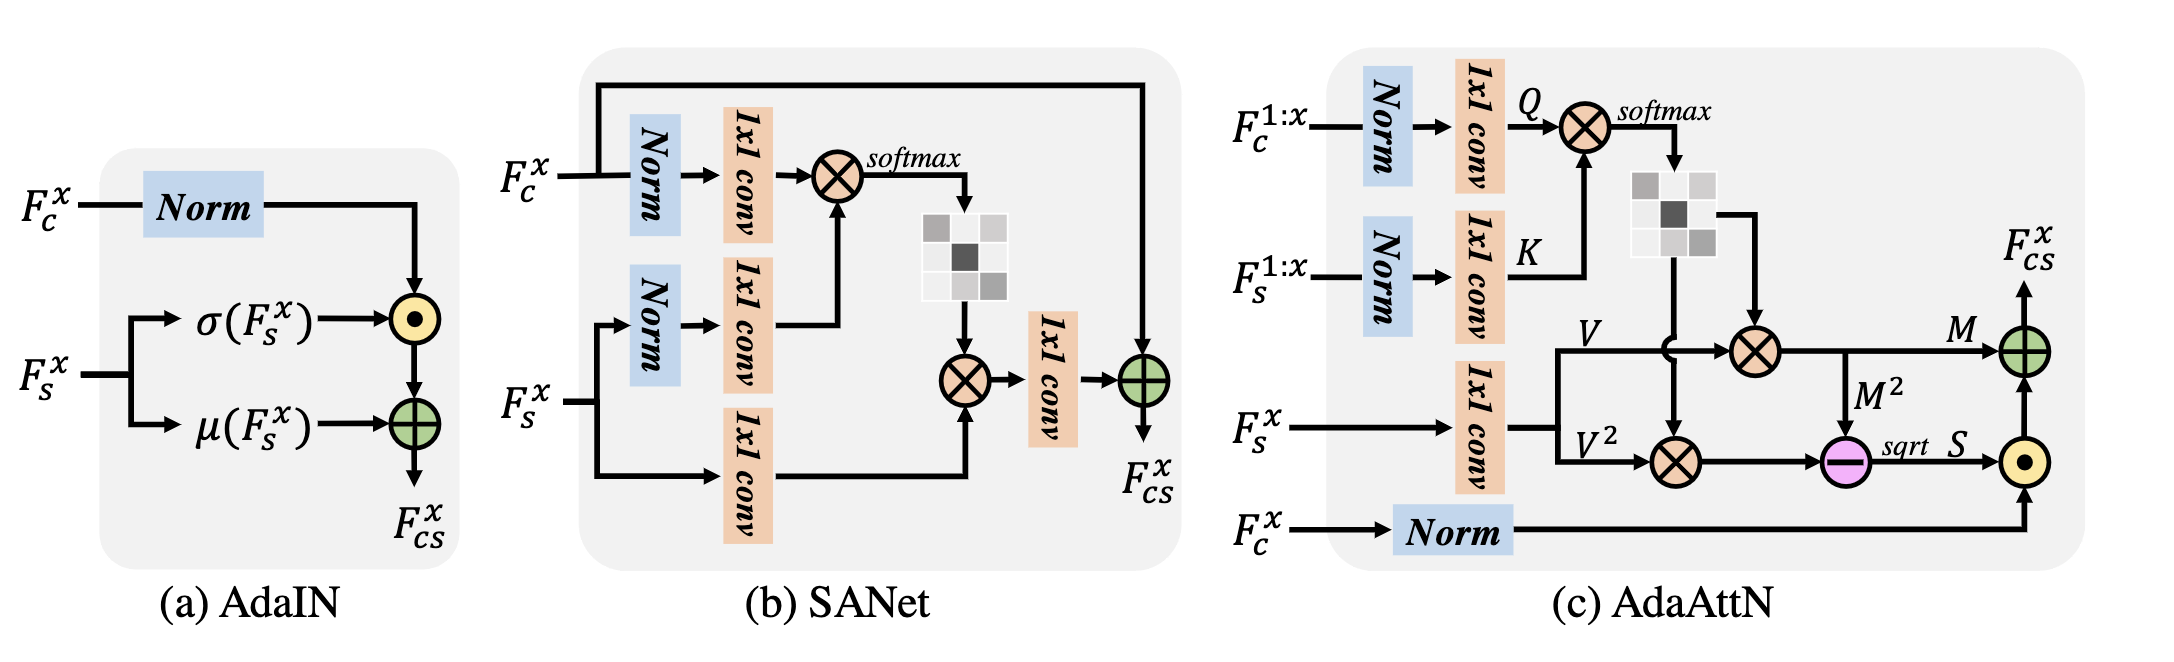
\includegraphics[width=\linewidth]{pics/diff_attn_p1}
    \caption{\label{fig:diff_adain_sanet_adaattn}三种方法在计算上的差别示意图~\cite{liu2021adaattn}}
\end{figure}

AdaAttN的总体流程如下:首先从VGG编码器的低层到高层依次计算包含内容和风格特征的注意力图,其中注意力机制是逐层计算的,用来衡量内容和风格特征之间的相似性。
随后基于注意力图计算风格特征的加权均值和标准差。最后使用自适应归一化内容特征实现特征分布对齐。
针对SANet的问题,还有一些人对他做出了相应的优化。其中Chen等人~\cite{chen2021artistic}提出一种具有两个对比性损失的内部-外部风格转移方法。
它保留了风格注意力网络,并且利用单个风格图像的内部统计特征来确定风格化图像的颜色和纹理模式,
同时,还利用大量风格图片的风格信息来学习人类感知上的风格偏好,
这使得其风格化图像中的颜色分布和纹理模式更加合理和谐。
同时间,Deng等人~\cite{deng2022stytr2}提出了一种称为 $StyTr^2$ 的基于Transformer的风格迁移模型。
该方法包括了一个新的感知内容位置编码(Content-Aware Positional Encoding,CAPE),其
中心思想是为图像风格迁移任务引入一种更加灵活和更高适应性的位置信息编码方式,
保证不同尺度的图像仍然有一致的空间关系。该模型认为风格图像不需要在编码期间严格保持位置关系,而内容图像需要,
故而该模型的风格图像编码器和内容图像编码器的唯一差别在于风格编码器没有应用CAPE。
经过训练以生成具有良好的输入内容图像结构和细节的风格化结果。Ma等人~\cite{ma2023rast}提出了一种迭代的架构,
从图像修复的角度解决内容泄漏问题。该方法通过多次的图像修复操作同时实现内容和风格信息的传输。
他们提出了两个新颖的损失函数:多修复损失和风格差异损失来确保更高的风格迁移质量。

\section{三维场景的风格迁移方法介绍}
近年来,随着科技的发展和人们对于娱乐需求的增加,人们对获取更优良的三维模型的需求也随之水涨船高。
精良的三维的场景不仅可以提供更真实、更具体、更立体的展现形式,还可以使用户获得更加沉浸式的体验和感受。
三维风格迁移技术的核心目标是在保持三维场景结构和多视角一致性的同时,将指定图像的艺术风格自然地应用到三维模型上,
这项技术能够为艺术家和设计师提供强大的工具,使他们能够比较轻松地将特定的艺术风格应用到3D的场景环境中,改变场景的显示属性。
三维场景的风格迁移现有的研究基础较为丰富,从场景的表达方式上来看主要可以分为三类:基于显式三维数据表示的风格迁移方法、基于隐式神经辐射场
(Neural Radiance Field,NeRF)表示~\cite{mildenhall2021nerf}的风格迁移方法、基于三维高斯飞溅(3D Gaussian Splatting,3DGS)表示~\cite{kerbl20233d}的风格迁移方法。下面将逐一进行介绍。


\subsection{基于显式三维数据表示的风格迁移方法}
最早的方法是使用点云或者三角形网格来对真实场景进行建模。Huang等人~\cite{huang2021learning}使用VGG-19的编码器提取出模型的特征和风格图像的特征,
并且使用了一种新颖的聚合算法把特征融入,并且使用经过训练的解码器渲染生成新的风格化视图。Mu等人~\cite{mu20223d}的思路同Huang等人相似,
但是使用AdaAttN结合UNet网络进行单图的风格化新视角生成。尹等人~\cite{yin20213dstylenet}提出了3DSTYLENET,
它由两个主要网络组件即几何和纹理风格传输网络组成。首先在一组无纹理形状上预训练3D几何样式传递网络,
在图像数据集上预训练纹理样式传递网络。然后将几何和纹理进行联合优化。 
通过将形状和纹理样式从一个纹理网格转移到另一个纹理网格来创建 3D 网格的新颖几何和纹理变化。
但是这种方法的性能受到几何重建方法本身的质量的限制。随着后来新的高效的几何重建方法被提出,使用显式三维数据用于场景风格迁移的方法也逐渐在性能上不如新方法了。
\subsection{基于隐式神经辐射场表示的风格迁移方法}
相比而言,神经辐射场NeRF的提出很好地改善了几何重建领域的新视图合成质量差、表示方式不灵活、训练较慢等问题,具有重要的意义。
为了更有利于理解,本文拟先对该方法进行一个全面的介绍,然后再介绍基于NeRF表示的风格迁移方法研究现状。


%2.2.2.1
\paragraph{NeRF方法介绍}
NeRF方法~\cite{mildenhall2021nerf}由谷歌高级研究科学家Jon Barron在2020年首次提出,是一种基于深度学习的三维场景重建和渲染方法,它通过神经网络存储场景的连续体积密度和颜色,
从而实现从多视点的二维图像数据中恢复出逼真的三维场景。NeRF的核心在于使用一系列从不同角度拍摄的图片来训练一个小型的神经网络,
该网络能够预测从任意位置以任意视角观看场景时的体积密度和颜色。把物体看作一团可以自发光的粒子,这些粒子具有颜色C,密度$\sigma$两个属性。
使用现有的照片对体空间内粒子的密度和颜色进行预测,保存这些信息。在渲染其他视角时,使用新视角的位置和方向信息通过神经网络得到颜色和密度属性信息进行推理,就能得到新视角下该场景的照片。NeRF的流程如\autoref{fig:nerf_show}所示:
\par 具体来说,NeRF要解决的问题就两个:
% \par 1. 如何通过现有的照片得到空间中密度与颜色的分布。
% \par 2. 如何利用这些数据,得到任意角度的照片。
\begin{enumerate}
    \item 如何通过现有的照片得到空间中密度与颜色的分布。
    \item 如何利用这些数据,得到任意角度的照片。
\end{enumerate}
\begin{figure}[htbp]
    \centering
    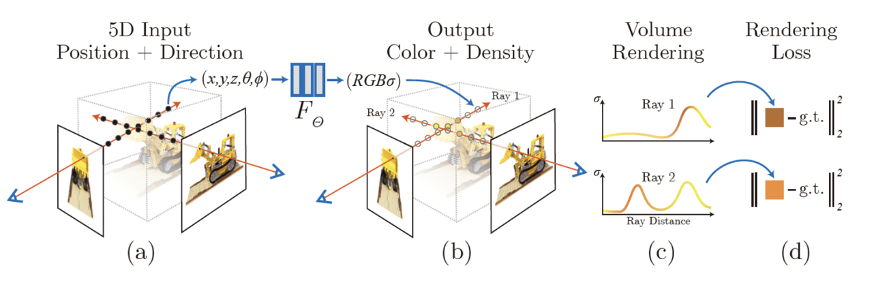
\includegraphics[width=\linewidth]{pics/nerf.png}
    \caption{\label{fig:nerf_show}NeRF方法的流程图~\cite{mildenhall2021nerf}}
\end{figure}



对于问题2,可以认为,从某一点看过去,这一点的颜色应该由经过这一点的光线上累积的颜色决定,想象每条光线经过其路径上的一个个小球到达最终像素上,
最终这些小球以自己的属性参与影响像素的颜色,这一计算可以用\autoref{equ:nerf_color_predict}表示:
% \begin{figure}[htbp]
%     \centering
%     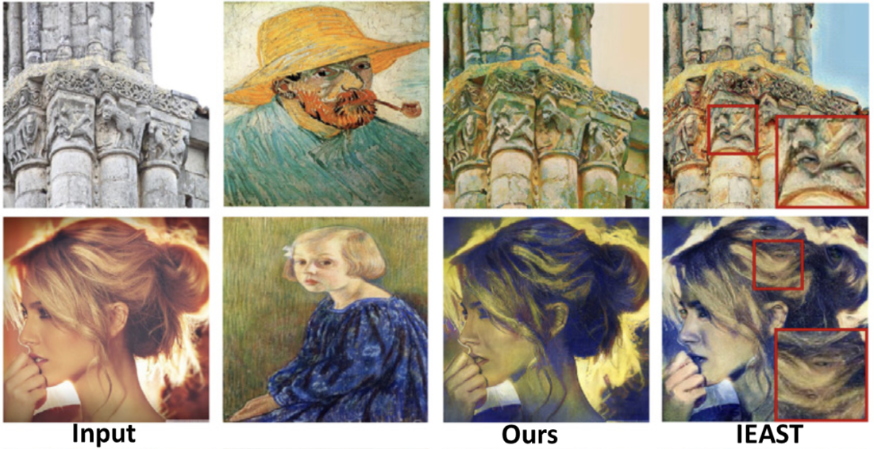
\includegraphics[width=\linewidth]{pics/pic_3.1.1}
%     \caption{\label{fig:pic_3.1.1}三种方法在计算上的差别示意图}
% \end{figure}
% aaa
% \begin{figure}[htbp]
%     \centering
%     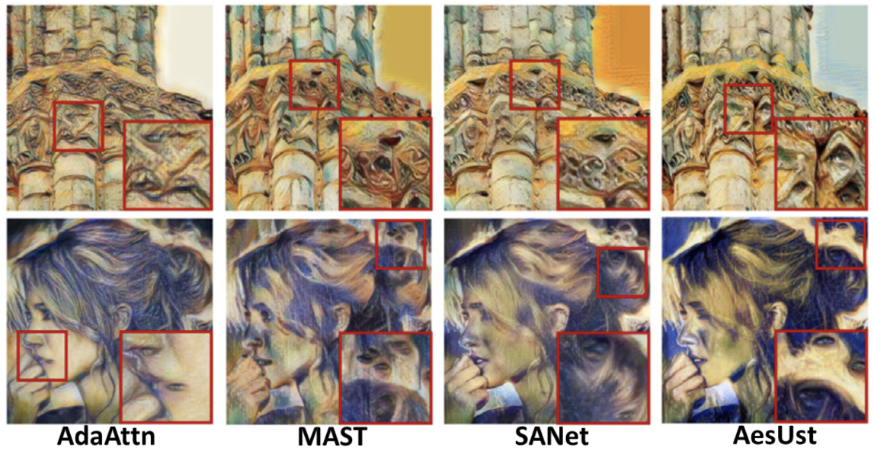
\includegraphics[width=\linewidth]{pics/pic_3.1.2}
%     \caption{\label{fig:pic_3.1.2}三种方法在计算上的差别示意图}
% \end{figure}

% t_n
% \autoref{equ:nerf_color_predict}
\begin{equation}
    \label{equ:nerf_color_predict}
    C^{p\text{redict}}(\mathbf{r})=\int_{t_n}^{t_f}T(t)\sigma(\mathbf{r}(t))\mathbf{c}(\mathbf{r}(t),\mathbf{d})dt
\end{equation}
其中$t_n$和$t_f$分别代表相机光线的近界和远界,$\mathbf{r}(t)=o+td$表示光线,$\sigma(t)$表示t处的密度,$\mathbf{c}(\mathbf{r}(t),\mathbf{d})$表示在$\mathbf{r}(t)$处以视角d看过去的颜色值,
$T(t)=\exp{(-\int_{t_n}^t\sigma(\mathbf{r}(s))ds)}$表示t处的不透明度。


\par 对于问题1,NeRF构建了一个神经网络$F_\theta$,其网络架构如\autoref{fig:nerf_net}所示:
\begin{figure}[htbp]
    \centering
    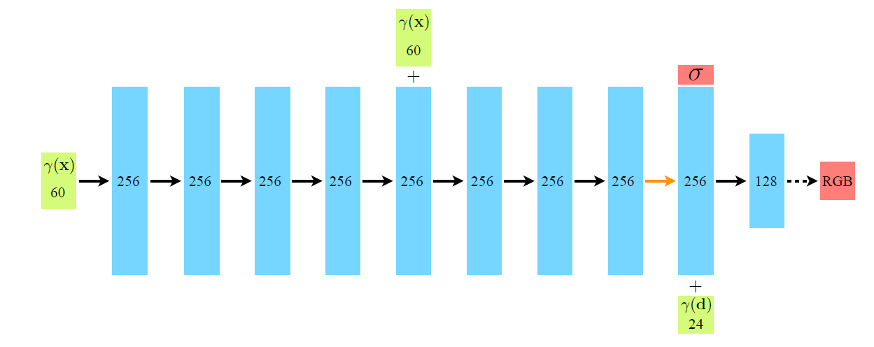
\includegraphics[width=\linewidth]{pics/nerf_net.png}
    \caption{\label{fig:nerf_net}NeRF方法的网络架构图~\cite{mildenhall2021nerf}}
\end{figure}




\par 输入为当前照片中,每个像素点看过来的角度,以及射线上采样点的坐标;输出为采样点上的颜色与密度。再利用上面的公式,计算得到预测的颜色 
% 再利用上面的公式,计算得到预测的颜色$\boldsymbol{C^{predict}}$,使用$\mathrm{MSE}(C^{ predict}-C)$作为约束进行训练。
\(\boldsymbol{C^{\text{predict}}}\),
并且使用 $MSE(\boldsymbol{C}^{\text{predict}} - \boldsymbol{C})$ 作为约束进行训练。
但是,考虑到输入的信息粒度太粗,直接在神经网络中输入坐标与角度信息只有6维数据,网络可能无法提取到一些比较细微的差别,训练效果并不好。
我们可以这么理解,对于某些场景下的同一点,以不同角度看过去,这个角度值的变化可能并不大,但是看到的颜色差别很大。
\par 为了提取到高频信息、增强模型的学习和表示能力,需要对输入进行增强。NeRF采用了位置编码的方法,将3维空间位置坐标和角度信息使用正弦余弦函数进行编码,
增强后输入变为如\autoref{equ:nerf_pe}所示:

% \begin{equation}
%     \label{equ:nerf_pe}
%     (x,y,z)\to(x,y,z,sin(2^0,x),sin(2^0,y),sin(2^0,z),cos(2^0,x),cos(2^0,y),cos(2^0,z),...sin(2^{n-1},x),sin(2^{n-1},y),sin(2^{n-1},z),cos(2^{n-1},x),cos(2^{n-1},y),cos(2^{n-1},z)(\theta,\phi)\to(\theta,\phi,\sin{(2^0,\theta)},\sin{(2^0,\phi)},\cos{(2^0,\theta)},\cos{(2^0,\phi)},...sin(2^{m-1},\theta),sin(2^{m-1},\phi),cos(2^{n-1},\theta),cos(2^{n-1},\phi))
% \end{equation}
\begin{equation}
    \label{equ:nerf_pe}
    \begin{aligned}
        (x,y,z) \to & (x,y,z, \sin(2^0 x), \sin(2^0 y), \sin(2^0 z), \cos(2^0 x), \cos(2^0 y), \cos(2^0 z), \ldots, \\
                    & \sin(2^{n-1} x), \sin(2^{n-1} y), \sin(2^{n-1} z), \cos(2^{n-1} x), \cos(2^{n-1} y), \cos(2^{n-1} z)) \\
        (\theta,\phi) \to & (\theta,\phi, \sin(2^0 \theta), \sin(2^0 \phi), \cos(2^0 \theta), \cos(2^0 \phi), \ldots, \\
                          & \sin(2^{m-1} \theta), \sin(2^{m-1} \phi), \cos(2^{m-1} \theta), \cos(2^{m-1} \phi))
    \end{aligned}
\end{equation}
在实际操作中,一般取n=10,m=4,则最后输入MLP中的\(\gamma(\mathrm{x})\)和\(\gamma(\mathrm{d})\)维度可以得到分别是60和24。
	经过训练的NeRF模型,其中存储了一个场景的隐式信息,只要给定新视角的相机参数,可以很方便地用它进行新视角图片的渲染合成,而该方法也为三维场景的渲染提供了一个更强大的技术路线。


\paragraph{基于隐式神经辐射场表示的风格迁移方法综述}
较早把NeRF技术结合风格迁移并且取得较好效果的一个方法是Zhang等人~\cite{zhang2022arf}提出的风格化辐射场
(Artistic Radiance Field,ARF),它是一种新的可以将艺术特征从单个 2D 图像转移到完整的真实世界 3D 场景,
从而产生忠实于风格图像的艺术新颖视图渲染的方法。
该方法利用通过真实场景预训练的辐射场,并通过匹配从输入的2D风格图像中提取的特征将其转换为艺术辐射场,
从而通过渲染获得高质量的风格化新颖视图合成。它提出了两个贡献点。
首先,考虑到直接使用先前基于VGG的风格损失将包括风格图中诸如笔触、笔画等属性的丰富的视觉细节直接转移到3D场景是具有挑战性的,
因为由这种损失测量的风格信息通常基于全局统计特征、不一定能够以视图一致的方式很好地捕获局部细节这一问题,
作者提出了一个新的风格损失:最近邻特征匹配损失(Nearest Neighbor Feature Matching,NNFM)
以一致地跨多个视点将复杂的高频视觉细节从2D风格图像转移到由辐射场参数化表示的3D场景。该损失函数的公式如\autoref{equ:nnfm}所示:
\begin{equation}
    \label{equ:nnfm}
    \ell_{\mathrm{nnfm}}(F_{\mathrm{render}},F_{\mathrm{style}})=\frac1N\sum_{i,j}minD(F_{\mathrm{render}}(i,j),F_{\mathrm{style}}(i^{\prime},j^{\prime}))
\end{equation}

其中$F_{render}$和$F_{Style}$分别是渲染后的图和风格图经过VGG-19编码器后得到的特征,
$F_{\mathrm{render}}(i,j)$代表特征图$F_{render}$在第(i,j)像素位置的特征向量,
N是$F_{render}$的像素数,$D(v_1,v_2)$计算两个向量$v_1$,$v_2$之间的余弦距离,其计算方式如\autoref{equ:cosine_distance}所示。
简而言之,对于$F_{render}$中的每个特征,该损失尝试最小化其到样式图像的VGG特征$F_{Style}$在VGG的特征空间中最近邻的余弦距离。
\begin{equation}
    \label{equ:cosine_distance}
    D(v_1,v_2)=1-v_1^Tv_2/\sqrt{v_1^Tv_1v_2^Tv_2}
\end{equation}


以上方法依然存在一个显著影响训练速度的问题,因为计算NNFM损失或者VGG特征损失的时候必须使用全分辨率图像,而不是图像的分块,而NeRF体渲染全分辨率图像的时候消耗大量内存。
为了解决这一问题,Zhang等人~\cite{zhang2022arf}还提出了一个叫做“延迟反向传播”的方法,该方法通过以补丁方式累积缓存的梯度,
使场景参数能够以一个内存高效的方式在全分辨率图像上计算损失。为了追求更快的风格化速度,
Li等人~\cite{li2023instant}提出了快速神经辐射场风格化(Instant Neural Radiance Fields Stylization),
他们的方法使用InstantNGP中~\cite{muller2022instant}提出的多分辨率哈希编码。首先,他们将InstantNGP中的位置编码器分为两部分:
内容和样式位置编码器。使用位置编码器,该网络可以在不到 10 分钟的时间内训练两个场景。
在对正常场景合成进行训练后,他们以内容和样式体素网格特征作为参考,在新视图合成的位置编码特征上执行AdaIN,并且将调整后的结果用于颜色预测,将未调整的结果用于密度预测。
该方法在保持相似的风格化质量的基础上实现了很大的速度提升。

\par 与Zhang等人同时期, Chiang等人~\cite{chiang2022stylizing}也提出了一种很新颖的保证风格化多视图一致性的方法。
他们使用超网络接受风格特征向量,并且据此输出该场景的NeRF模型的颜色MLP的参数。训练的时候首先训练NeRF模型的几何特性,
再对多个视角、多个风格分别最小化风格和内容损失以训练超网络习得风格的解码能力。
最终获得一个可以进行零样本场景风格迁移的网络。但是上述方法都无法捕捉较为局部的笔触风格信息。

\par Chen等人~\cite{chen2023testnerf}则考虑根据文本提示词来风格化场景并生成具有一致性的任意新视图。这是一个很有想法的尝试。
为了解决这个问题,他们首次设计了一个高效的文本驱动模型用于 3D 风格迁移,名为 TeSTNeRF。
通过跨模态学习对文本进行风格化:他们保留了Chiang等人~\cite{chiang2022stylizing}的超网络控制思路,
并利用高级文本编码器~\cite{radford2021learning}嵌入文本以控制 3D 风格迁移并在潜在空间中对齐输入文本并输出风格化图像。
此外,为了获得更好的视觉效果,他们引入了风格监督、从风格图像中学习特征统计并利用 2D 风格化结果来纠正突然的颜色溢出,
取得了较好的效果。但是文本相对于图像,其对于风格的描述能力有限,这也导致了在有的场景上风格化结果表现力不足等问题。

\par Chen等~\cite{chen2024upst}受到Chiang等人~\cite{chiang2022stylizing}的启发,也采用了超网络和超网络层学习风格潜向量的思想设计了UPST-NeRF,
但是他们没有直接修改隐式辐射场中存储的颜色信息,而是在查询阶段的MLP中对颜色进行修改,可以视为是一种“增量”的思想,
也可以看作是一个颜色解码器,对后面的方法影响深远。此外,为了更好地服务于真实感图像的风格化,
他们训练了一个 2D 逼真图像的风格迁移网络来处理不同视图下的真值 RGB 以获得训练的目标,
在训练的时候对于每个视角每个风格都应用该网络获取风格化结果并用其来约束预测的颜色值。
但是他们这些方法都不能做到在零样本迁移的同时还能保持较高的风格化质量。
为此,Liu等人~\cite{liu2023stylerf}提出了StyleRF,通过在辐射场的特征空间中执行风格迁移来尝试解决风格化的高精度重建、
高质量风格迁移、零样本快速迁移三方困境问题。具体来说,作者设计了采样不变的内容转换和延迟样式转换
(Sampling-Invariant Content Transformation 和Deferred Style Transformation),
前者通过严谨的数学论证消除对采样点批次的整体统计特征的依赖来确保多视图的一致性,
而后者通过将样式转换推迟到 2D 特征图渲染阶段,大大提高了风格化效率。这个算法实现了很好的风格迁移效果和效率,
但是随着三维高斯飞溅方法的提出和应用,性能和效果逐渐被超越。下文将详细阐述3DGS方法和基于其的场景风格迁移方法概述。


\subsection{基于三维高斯飞溅表示的风格迁移方法}
三维高斯飞溅(3D Gaussian Splatting,3DGS)方法由Kerbl等人~\cite{kerbl20233d}在2023年提出,是多视角重建方面的突破性工作。它的特点在于使用3D高斯分布来表示场景,并且设计了一个创新的流水线,它既能够对高斯点进行高速的投影和渲染,还能可以执行遵循可见性排序的各向异性飞溅,并通过跟踪和遍历尽可能多的排序后的高斯点来实现快速准确的反向传播。同时,该方法有着卓越的渲染速度(能够以较少的训练时间,实现SOTA级别的NeRF的实时渲染效果,且可以以 1080p 分辨率进行高质量的实时(≥ 30 fps)新视图合成)。下面对该方法进行详细的介绍。
\paragraph{3DGS方法介绍}
神经辐射场方法彻底改变了用多张照片或视频捕捉的场景进行的可视化合成。然而,实现高质量的可视化仍然需要使用大量的参数且训练和渲染速度缓慢的神经网络结构。
下面本段将对一种新颖的解决方案:3D 高斯飞溅技术进行一个简述。高斯飞溅是一种在90年代科学领域创建的渲染技术。
不过,它最近在2023年8月的 SIGGRAPH 2023上展示的实时场景可视化应用,让它再次流行起来。
该技术和NeRF的区别大体上可以叙述为:对于场景表示,NeRF采用隐式辐射场表示,并且通过MLP查询得到某一位置的属性,而3DGS采用显式的高斯球进行表达,直接存储其特征属性;
对于渲染,NeRF是非常典型的backward mapping过程,即计算出每个像素点受到每个体素影响的方式来生成最终图像,对每个像素,投射出一条光线,并累积其路径上的颜色和不透明度。
而3DGS是forward mapping的过程,将每个体素视作一个模糊的球,投影到屏幕上。在溅射过程中,计算出每个体素如何影响每个像素点。
3DGS的优势在于:3D高斯表示支持渲染最先进的视觉质量,且拥有相对NeRF显著更短的训练时间,而基于分片的飞溅投影解决方案和使用CUDA做特别优化的特殊流水线确保了渲染的高速度和高分辨率。
每个高斯球包括的属性有位置(平均值$\mu$):存储了位置(XYZ)的空间坐标,协方差矩阵($\Sigma$):表征高斯球的旋转和缩放特性,不透明度($\alpha$):
代表每个高斯球的不透明程度,球谐 (SH) 系数:存储了每个高斯球的颜色特征。采用SH系数这样的各向异性属性可以允许非常灵活的优化机制。
该方法高效率的关键在于作者提出了一个基于分片的快速光栅化(tile-based rasterizer),它允许以$\alpha$-blending方式混合各向异性的溅射。
该快速光栅化器还包括实现了一个快速的反向传递,允许对任意数量的混合高斯进行有效的反向传播。本文提供的方法流程如\autoref{fig:3dgspipline}所示:

\begin{figure}[htbp]
    \centering
    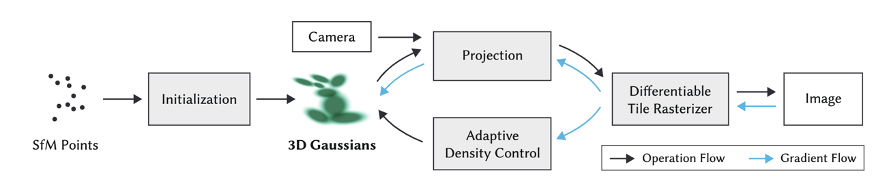
\includegraphics[width=\linewidth]{pics/3dgspipeline.png}
    \caption{\label{fig:3dgspipline}3DGS方法的管线图~\cite{kerbl20233d}}
\end{figure}

具体来说,本文提出的方法优化从稀疏的SfM点云开始,初始化创建一组3D高斯,其将几何形状建模为一组不需要法线的3D高斯曲线。
提出的高斯分布由一个完整的三维协方差矩阵\(\Sigma=RSS^TR^T\)定义在世界空间中,$R$和$S$分别是旋转矩阵和缩放矩阵参数,以平均值μ为中心。其可以表达如\autoref{equ:3dgs_equ_main}所示:
% \autoref{equ:nerf_color_predict}
\begin{equation}
    \label{equ:3dgs_equ_main}
    G\left(x;\mu,\Sigma\right)=\frac1{\sqrt{(2\pi)^k\mid\Sigma\mid}}\exp\left(-\frac12(x-\mu)^T\Sigma^{-1}(x-\mu)\right)
\end{equation}
\par 随后,在渲染阶段,采用把3D高斯投影到2D平面上的方式,并使用提出的快速的基于分片的渲染器对此投影后的结果进行渲染。该渲染器使用了高度优化的光栅化管线和高性能的CUDA自定义内核,实现了快速的整体渲染和快速排序的目标,它有着极快的渲染速度和较小的额外内存消耗,可以对各种场景进行实时渲染。
\par 由于这一方法是从SfM初始化的,其高斯球的数量和密度必然不够精确。因此作者还提出了高斯函数的自适应性控制,简单来说,对于处于重建不足区域的小高斯函数,需要覆盖必须创建的新几何区域,因此采用克隆高斯球并且向位置梯度方向移动它的方法。对于高方差区域中的大高斯分布,它需要被分割成两个小高斯分布,并且把它们的尺寸都统一缩小一定值然后参与新一轮次的优化。
\paragraph{基于3DGS表示的风格迁移方法综述}
在3DGS方法的基础上,结合风格迁移技术,众多研究者加以研究和探索,开发出了一些很有效果的3D场景风格迁移算法。首先Chen等人~\cite{chen2024gaussianeditor}提出了GaussianEditor,它是一个基于3DGS表示的快速可控三维可编辑场景的工作,它主要是用于场景编辑,但也可以用于风格迁移任务。它引入了高斯语义跟踪,从而实现更详细和有效的对象编辑控制。同时它还提出了分层的高斯飞溅(HGS),这是一种新的GS表示,根据高斯点的致密化轮次进行分类并对它们进行逐步收缩的限制,这能够在高度随机的生成引导下更稳定地收敛到细化的结果。同时,它设计了一种用于高斯飞溅的3D修复算法,该算法可以快速去除和添加对象,更方便执行可控的场景编辑工作。但是本工作主要依靠预训练的多模态大语言所学到的丰富先验知识引导风格化操作,相比于使用蕴含丰富细节、内容信息的图像引导的风格迁移工作稍显不足,但是这是一个很好的探索。

\par 第一个真正意义上使用3DGS的表示用于图片引导的场景风格迁移工作是Sahara等人~\cite{saroha2024gaussian}提出的GSS,他们提出使用InstantNGP中提出的多分辨率哈希编码来对已经初始化完成的高斯点集进行升维表示,多分辨率哈希编码在每一层都是独立的,并且高度适应所需的最佳分辨率。因此,它在训练期间实现了更快的收敛,不会阻碍推理速度,并促进更高级别的细节,这有利于使用 3DGS 表示的风格化任务。随后,GSS提出了一个3D颜色模块,把每个风格化图的潜向量和每个高斯点的查询结果拼在一起并且使用一个MLP进行计算得到高斯点风格化后的颜色。该方法能够准确地生成场景中每个 3D 高斯的风格化颜色,并且以很高的速度渲染生成新的视角,这得益于3DGS本身相对于NeRF方法的速度优势。但是由于该方法仅使用AdaIN来做风格化监督,其生成的场景依然不太考虑风格图像的笔触、线条特征等艺术问题。

\par Zhang等人~\cite{zhang2024stylizedgs}提出了StylizedGS,它可以支持可调整的控制因子,以改变控制强度,并提出了一种GS过滤器来消除重建中的会影响风格化效果的漂浮物,然后引入基于最近邻的样式损失NNFM Loss,通过微调3DGS的几何和颜色参数来实现风格化,同时提出了一种具有其他正则化的深度保存损失,以防止几何内容被大幅度修改。本文的高斯点风格化操作通过颜色的直方图匹配算法实现。

\par Yu等人~\cite{yu2024instantstylegaussian}提出InstantStyleGaussian,该方法主要依赖于图像提示,并利用文本辅助生成训练数据集。总的来说该方法使用图像的条件扩散模型用于迭代更新训练数据集图像,然后对重建的场景模型进行微调以匹配参考编辑的图像样式,最终生成符合艺术风格的场景,同时保持3D一致性。该方法实现了具有更高质量风格化的3D 场景风格迁移,提高了速度和性能。但是该方法的效果依赖于图像的扩散模型的性能。相信随着更强大的图像处理扩散模型的出现,该方法更好的风格化效果将会可以期待。

\par Liu等人~\cite{liu2024stylegaussian}提出了StyleGaussian,它允许以每秒10帧的速度将任何图像的样式即时地迁移到3D场景中。利用3D高斯飞溅(3DGS),StyleGaussian在不影响其实时渲染能力和多视图一致性的情况下实现了样式转移。它把三维场景风格迁移的通用流程总结为:特征嵌入、风格迁移和解码渲染。最初,2D 图像的VGG场景特征被嵌入到重建的3D高斯中。接下来,根据参考风格图像对嵌入的特征进行变换。最后,将转换后的特征解码为风格化的 RGB。StyleGaussian 有两种新颖的设计。第一个是一种有效的特征渲染策略,它显著减少了内存消耗。它首先渲染低维特征,然后将它们映射到高维特征,同时嵌入VGG 特征,这样解决了 3DGS 不能够渲染高维内存密集型特征的问题。第二个是基于K最近邻的 3D CNN解码器。这种解码器直接在3D空间中工作,可以很好地保持多视图一致性并且不影响3D高斯渲染的速度。

\par \(\text{Kovács}\)等人~\cite{kovacs2024g}提出了G-style,该文章认为现有的基于3DGS的场景迁移方法不会改变表示场景的高斯的位置和形状,这将会导致场景的某些区域的分辨率较低。除了上述问题外,所有 3D 风格迁移方法只关注从风格图像中转移高频模式,例如笔触或颜色统计。然而,图像风格的概念更加微妙,并且与图像有很大不同。G-style首先在预处理步骤中删除了具有大投影区域或高度拉长形状的不良高斯点,并且限制只使用球谐函数的第0阶以保证只有漫反射属性。为了确保最终的风格化3D场景与原始风格图像之间的颜色分布相似,在算法开始时,将真实图像与风格图像的颜色的均值和协方差矩阵进行匹配。随后作者结合了几个精心设计的损失来保留图像中风格的不同比例,同时保持原始场景内容的完整性尽可能高。为了更好的提高某些低分辨率部分的风格化质量,在风格化过程中通过跟踪风格化颜色的梯度来拆分在场景中需要额外的细节的高斯。为了克服高斯点数量过多这个问题,在风格化过程中,作者还添加了一个高斯点的微调步骤,根据它们的风格属性的梯度周期性地拆分高斯函数。

\par 为了获得更高质量的指定区域风格化,Jain等人~\cite{jain2024stylesplat}提出了StyleSplat,这是一种轻量级的方法,用于从参考样式图像中对由3D高斯表示的场景中的部分3D对象进行风格化。该方法首先使用 3D 高斯溅射学习场景的逼真表示,同时使用语义分割大模型SAM~\cite{kirillov2023segment}联合分割单个 3D 对象。随后使用最近邻特征匹配损失NNFM来微调所选对象的高斯属性,将它们的球谐系数与样式图像对齐,以确保一致性和视觉吸引力。StyleSplat允许场景中多个对象的快速、可定制的样式转移和局部风格化,每个对象都有不同的样式。

\par 上述方法除了最后提出的几个同期工作以外,均可以在性能方面继续提升,以让风格化效果更加精致、支持更快的零样本风格迁移等。这正是本文的目标之一,相关细节将在本文第四章予以详细说明。

\section{对比学习技术}
由于本文所提出的方法需要使用到对比学习方法来学习从风格化到风格化的关联,故本文在此对这一技术进行一个介绍。对比学习由三个关键要素组成:查询、正例样本和负例样本。对比学习背后的基本思想是鼓励相似的实例在学习的嵌入空间中被映射得更近,同时将不相似的实例推得更远。通过将学习视为一项辨别任务,对比学习允许模型捕获数据中的相关特征和相似性。对比学习由以下几个步骤构成:数据增强、特征提取、投影网络、对比学习的目标、损失函数、训练和优化、评估。
\par 数据增强:对比学习方法的初始阶段是数据增强。数据增强的主要目标是增强数据的异构性,从而将模型引入相同实例的多个视角。此步骤涉及应用各种转换技术,包括裁剪、翻转、旋转和额外扰动来生成一系列数据表示。实例的多样化有助于确保对比学习模型能够吸收相关信息,而不管输入数据中存在的变化。
\par 特征提取:数据增强之后,对比学习过程使用编码器网络将增强的实例转置到潜在表征空间来发挥作用。这种能力对于模型区分相似实例和不相似实例至关重要。编码器网络的架构通常由先进的神经网络模型构成,例如用于图像数据集的卷积神经网络 (CNN) 或用于序列数据的循环神经网络 (RNN)等。
\par 投影网络:投影网络负责将编码器网络的输出映射到为更紧凑、更低维的空间。此阶段对于增强模型的辨别能力至关重要。通过将表示转移到低维空间中,投影网络有效地减轻了数据复杂性和冗余度。这种减少对于在数据集内实现相似实例和不相似实例之间的更明显区分起着关键作用。
\par 对比学习的目标:将增强实例编码并投影到嵌入空间后,即可系统地应用对比学习目标。
该目标的设计有两个重点:首先,最大化来自同一样本的实例之间的一致性;其次,最小化来自不同样本的实例之间的一致性。
这种策略方法激励模型在表征空间中拉近具有相似性的实例,同时疏远不相似的实例。实例之间的相似度量化通常采用距离度量,其中欧几里得距离或余弦相似度是常用的度量。
\par 损失函数:对比学习任务有许多不同的损失函数,每个损失函数的设计目的都是为了促进获取能够巧妙地概括数据集内基本相似性和差异性的表示。
可用于风格迁移领域比较著名的损失函数有:ContraGAN~\cite{kang2020contragan}提出的一个条件对比学习损失函数(Conditional Contrastive Loss,2C loss),
它能学习样本到类和样本到样本的关系。OpenAI~\cite{radford2021learning}提出的对比语言-图像预训练损失(CLIP Loss)构建了语言和图像之间的有效关系。
CLIP通过对比学习的方式,将图像和文本嵌入到同一个语义空间中,使得模型能够理解图像和文本之间的语义关系。
CLIP模型的核心思想是通过最大化图像表示与其相应文本描述之间的一致性,来预训练一个能够同时理解图像和文本的模型。
对比学习是CLIP模型的核心,它通过比较正样本(匹配的图像-文本对,即图中对角线上N个匹配的图像-文本对)和负样本(不匹配的对,即$N^2-N$个没有匹配的图像-文本对)来训练模型。
这种学习策略使得模型能够学习到图像和文本之间的复杂关系,而不仅仅是简单的特征对应。CLIP的对比学习框架提高了模型对视觉和语言数据的泛化能力。
受此启发,可以把CLIP模型的思想运用到图像的风格迁移中来。\autoref{fig:clip_intro}是CLIP的说明示意图。CLIP 可以生成良好的视觉表示,
可以非常轻松地迁移到许多计算机视觉领域的基准数据集,从而实现与有监督的基线方法相媲美的结果。
\begin{figure}[htbp]
    \centering
    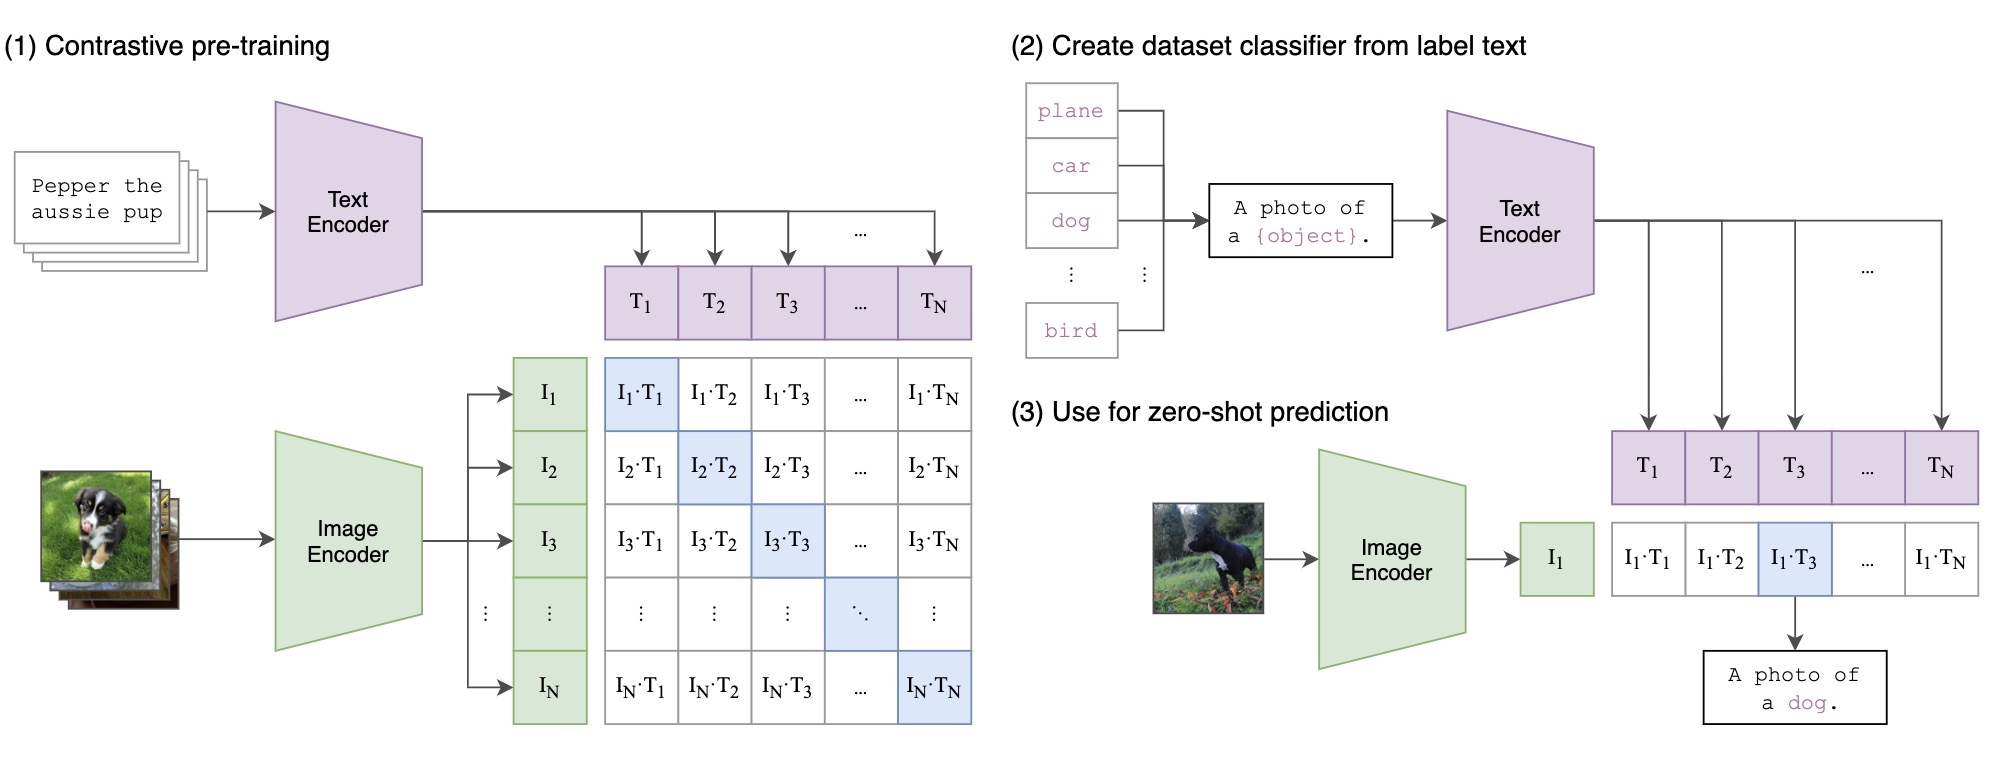
\includegraphics[width=\linewidth]{pics/clip_introduction.jpg}
    \caption{\label{fig:clip_intro}CLIP方法示意图~\cite{radford2021learning}}
\end{figure}
\par 训练和优化:在定义损失函数后,模型会使用大量数据集(主要是未标记的数据集)进行训练。这个训练过程是迭代的,通过不断更新模型的参数以最小化损失函数。这种迭代优化逐步细化所学习到的表示,从而增强模型有效区分和区分相似和不相似实例的能力。
\par 在风格迁移的领域,Chen等人~\cite{chen2021artistic}首先基于预训练的VGG模型构建正样本和负样本,以学习风格化到风格化的关系。Zhang等人~\cite{zhang2022domain}全面介绍了使用视觉特征进行风格表示的对比学习,以表示任意风格转移的风格。Wu等人~\cite{wu2022ccpl}设计了一种通用的对比相干保持损失来学习局部斑块。
CLIPstyler~\cite{kwon2022clipstyler}引入了一个文本引导的合成模型,可以根据特定的文本传输图像的风格。这些方法都在一定程度上保留了内容图像的内容并增强了风格化图像的风格,给本文提供了思路上的启发。

\section{评价指标}
风格迁移是一类试图合成艺术风格化的视觉媒介的方法。为了评估风格化的性能结果,使用了多种评估方法和指标,包括统计参与者主观判断的人类视觉效果评估,
以及客观评估算法性能不同方面的大量定量计算指标。然而,对于能够保证结果可靠性的最合适和最有效的评价手段,
由于艺术风格这一概念的模糊性,和高度主观性,目前在客观指标的选用上还没有达成共识。
现用的计算指标试图量化内容留存率、风格相似性和整体效率这些因素。尽管有大量的评估方法,
但评估过程在NST算法之间是不同的。根据媒介的不同,也取决于一种方法旨在实现的特定进步或贡献,
每种风格转移方法都采用不同的评估程序。评估NST方法的产出所涉及的主观性,每种方法的特定意图和目标,
以及每种方法试图解决风格化问题的角度,使评估成为一项复杂而苛刻的活动。经过认真地调研,
决定本文的评估决定从主观和客观两个角度进行评估。其中主观角度采用欺骗分数(Deception Score)。
欺骗分数表示用户把生成的风格化鉴定为真实艺术图像的比率。
更高的分数意味着该风格化图像被更高比例人鉴定为真实风格化作品。
客观角度采用内容保真度(Content Fidelity,CF), 全局影响分数(Global Effects ,GE)和本地图样分数(Local Patterns ,LP)~\cite{wang2021evaluate}指标,
保证指标覆盖了感知属性和风格化表现这两个方面,用于二维图像风格迁移的效果评估,采用长短期一致性用于三维图像风格迁移的效果评估,
并且采用ArtFID~\cite{wright2022artfid}和结构相似性(Structural Similarity,SSIM)~\cite{wang2004image}等指标用于场景风格化后渲染得到的2D风格化图像的质量评估,
采用短程一致性和长程一致性(Short-range Consistency和Long-range Consistency)~\cite{lai2018learning}用于3D场景的风格化一致性质量评估,下文将对这些指标进行详细解释说明。
\par CF是用来衡量在多个尺度上对内容特征的忠实度。它基于这样一个看法:令人印象深刻的风格转移结果应该携带足够的风格特征,同时保留明显感知的内容结构。其公式如\autoref{equ:equ_cal_cf}所示:

\begin{equation}
    \label{equ:equ_cal_cf}
    CF(\vec{x},\vec{c})=\frac1N\sum_{l=1}^N\frac{f_l(\vec{x})\cdot f_l(\vec{c})}{\parallel f_l(\vec{x})\parallel\cdot\parallel f_l(\vec{c})\parallel}
\end{equation}
其中$\vec{c}$和$\vec{x}$分别是内容图像和风格化结果,\(f_l(\cdot)\)表示从第$l$层提取的特征激活。N是不同层的数量。
\par GE用来衡量全局相似性。在将转移的风格与风格图像进行比较时,人们经常首先欣赏全局效果。全局相似性将对人类视觉感知留下初步印象,
因此它是衡量风格化质量的重要因素。通过调查作者认为颜色和纹理更容易影响观察者的评估,因此全局效应 (GE) 因子应包括这两个方面,
即全局颜色 (GC) 和整体纹理 (HT)。对于GC的计算,直接比较颜色直方图的余弦相似度以利用RGB颜色空间中的颜色信息,其计算方式如\autoref{equ:equ_cal_gc}所示;对于HT的计算,
利用Gatys等人提出的~\cite{gatys2016image,gatys2017controlling}风格表示 (Gram 矩阵),这已被证明可以有效地表达图像的整体纹理。其计算方式如\autoref{equ:equ_cal_ht}所示:
\begin{equation}
    \label{equ:equ_cal_gc}
    GC(\vec{x},\vec{s})=\frac13\sum_{c=1}^3\frac{hist_c(\vec{x})\cdot hist_c(\vec{s})}{\parallel hist_c(\vec{x})\parallel\cdot\parallel hist_c(\vec{s})\parallel}
\end{equation}
其中$\vec{s}$是风格图像,\(hist_c(\cdot)\)表示由通道$c$得到的颜色直方图向量。
\begin{equation}
    \label{equ:equ_cal_ht}
    HT(\vec{x},\vec{s})=\frac1N\sum_{l=1}^N\frac{G(f_l(\vec{x}))\cdot G(f_l(\vec{s}))}{\parallel G(f_l(\vec{x}))\parallel\cdot\parallel G(f_l(\vec{s}))\parallel}
\end{equation}
其中$G(*)$表示Gram矩阵。由于认为这两个因素都是同等重要的,因此最后通过计算二者平均值得到GE分数,如\autoref{equ:equ_cal_ge}所示:
\begin{equation}
    \label{equ:equ_cal_ge}
    GE(\vec{x},\vec{s})=\frac12(GC(\vec{x},\vec{s})+HT(\vec{x},\vec{s}))
\end{equation}
\par LP指标的灵感来源于:在大致感知全局效果后,人们会放大观察一些局部风格模式的相似性,
如笔触、精美图案、详细的纹理等。
因此,定义了一个局部模式(LP)因子来衡量这一方面的质量。
受到人类评估中考虑的元素的启发,该LP 因子由两部分组成,一是直接评估局部模式对应物的相似性,
二是比较检索到的模式类别的多样性。一个好的风格化结果应该类似于风格图像,不仅在相应的局部模式中,而且在检索到的模式类别的多样性上。首先用神经网络对神经特征
\(f_l(\vec{x})\)和\(f_l(\vec{s})\)提取一组3 × 3的块(patch),记为\(\{\Phi_i^l(\vec{x})\}_{i\in n_x}\)和\(\{\Phi_j^l(\vec{s})\}_{j\in n_s}\),
其中$n_x$和$n_s$分别是内容图像和风格图像的块数。对于每一个\(\Phi_i^l(\vec{x})\),
根据如\autoref{equ:equ_cal_tmp_phi_cmi}所示的归一化相关度确定最匹配的样式块\(\Phi_{CM(i)}^l(\vec{s})\):

\begin{equation}
    \label{equ:equ_cal_tmp_phi_cmi}
    \Phi_{CM(i)}^l(\vec{s}){:}=\arg\max_{j=1,...,n_s}\frac{\Phi_i^l(\vec{x})\cdot\Phi_j^l(\vec{s})}{\parallel\Phi_i^l(\vec{x})\parallel\cdot\parallel\Phi_j^l(\vec{s})\parallel}
\end{equation}
随后可以定义LP为$LP_1$和$LP_2$两部分,如\autoref{equ:equ_cal_lp1}和\autoref{equ:equ_cal_lp2}所示:
\begin{equation}
    \label{equ:equ_cal_lp1}
    LP_1(\vec{x},\vec{s})=\frac1Z\sum_{l=1}^N\sum_{i=1}^{n_x}\frac{\Phi_i^l(\vec{x})\cdot\Phi_{CM(i)}^l(\vec{s})}{\parallel\Phi_i^l(\vec{x})\parallel\cdot\parallel\Phi_{CM(i)}^l(\vec{s})\parallel}
\end{equation}
其中\(Z=N\times n_x\),这一部分测量了\(f_l(\vec{x})\)和\(f_l(\vec{s})\)所对应的局部图样的相似性。
另一部分直接通过比较不同的神经块的类数目来定义。
\begin{equation}
    \label{equ:equ_cal_lp2}
    LP_2(\vec{x},\vec{s})=\frac1N\sum_{l=1}^N\frac{t_{cm}^l}{t_s^l}
\end{equation}
其中$t_{cm}^{l}$和$t_{s}^{l}$分别代表
$\{\Phi_{CM(i)}^l(\vec{s})\}$和$\{\Phi_j^l(\vec{s})\}$
中不同块的数量。考虑到两者一致的重要程度,最终可以得到总的LP分数如\autoref{equ:equ_cal_lp_all}所示:
\begin{equation}
    \label{equ:equ_cal_lp_all}
    LP(\vec{x},\vec{s})=\frac12(LP_1(\vec{x},\vec{s})+LP_2(\vec{x},\vec{s}))
\end{equation}
\par SSIM~\cite{wang2004image}是一个经典的评估指标,它从三个方面综合评价图像质量:亮度相似性、对比度相似性、结构相似性。它的计算流程如\autoref{fig:img_ssim_cal}所示:

\begin{figure}[htbp]
    \centering
    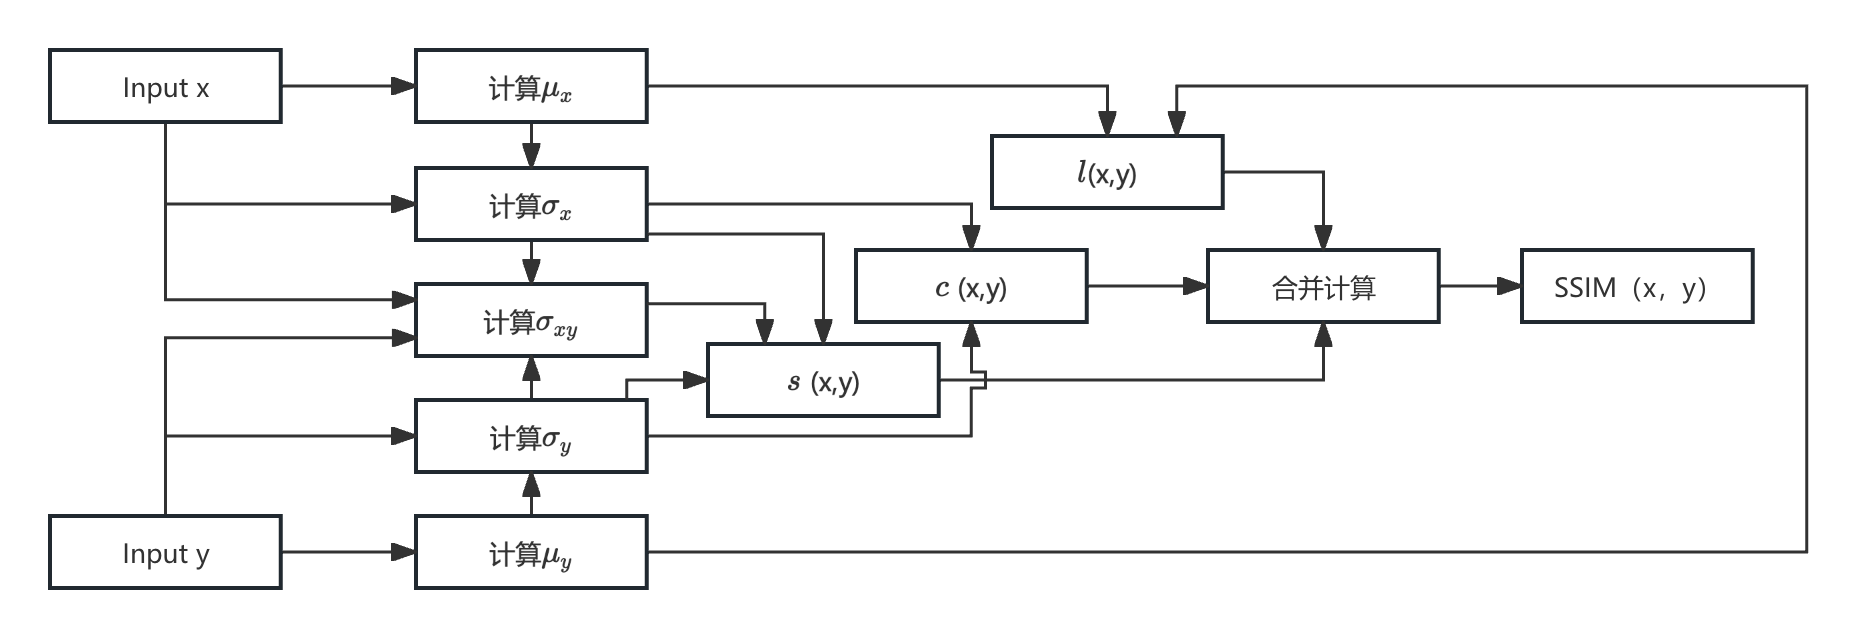
\includegraphics[width=\linewidth]{pics/ssim_cal.png}
    \caption{\label{fig:img_ssim_cal}SSIM计算示意图}
\end{figure}
在该图中的亮度相似性的定义如\autoref{equ:equ_cal_ssim_lxy}所示:
\begin{equation}
    \label{equ:equ_cal_ssim_lxy}
    \mathrm{l(x,y)=\frac{2\mu_x\mu_y+C_1}{\mu_x^2+\mu_y^2+C_1}}
\end{equation}
其中\(\mu_\mathrm{x}=\frac{1}{\mathrm{N}}\sum_{\mathrm{i}=1}^\mathrm{N} \mathrm{x_i}, \mu_\mathrm{y}=\frac{1}{\mathrm{N}}\sum_{\mathrm{i}=1}^\mathrm{N} \mathrm{y_i}, \mathrm{C_1}\)
是一个防止分母为零的常数。对比度相似性的定义如\autoref{equ:equ_cal_ssim_cxy}所示:
\begin{equation}
    \label{equ:equ_cal_ssim_cxy}
    \mathrm{c}(\mathbf{x},\mathbf{y})=\frac{2\sigma_\mathrm{x}\sigma_\mathrm{y}+\mathrm{C}_2}{\sigma_\mathrm{x}^2+\sigma_\mathrm{y}^2+\mathrm{C}_2}
\end{equation}
其中,\(\sigma_{\mathrm{x}}=\left(\frac1{\mathrm{N}-1}\Sigma_{\mathrm{i}=1}^{\mathrm{N}}\left(\mathrm{x}_{\mathrm{i}}-\mu_{\mathrm{x}}\right)^{2}\right)^{\frac12},\sigma_{\mathrm{y}}=\left(\frac1{\mathrm{N}-1}\Sigma_{\mathrm{i}=1}^{\mathrm{N}}\left(\mathrm{y}_{\mathrm{i}}-\mu_{\mathrm{y}}\right)^{2}\right)^{\frac12},C_{2}\)
的作用和\(C_1\)相同。结构相似性的定义如\autoref{equ:equ_cal_ssim_sxy}所示:
\begin{equation}
    \label{equ:equ_cal_ssim_sxy}
    \mathrm{s(x,y)=\frac{\sigma_{xy}+C_3}{\sigma_x\sigma_y+C_3}}
\end{equation}
其中,\(C_3\)的作用和\(C_2、C_1\)相同,都是为了防止分母出现零,而\(\sigma_{\mathrm{xy}}\)是x和y的协方差,其可以按\autoref{equ:equ_cal_ssim_covxy}计算:
\begin{equation}
    \label{equ:equ_cal_ssim_covxy}
    \sigma_{\mathrm{xy}}=\frac1{\mathrm{N}-1}\sum_{\mathrm{i}=1}^{\mathrm{N}}(\mathrm{x_i}-\mu_\mathrm{x})(\mathrm{y_i}-\mu_\mathrm{y})
\end{equation}
有了上述三个公式后,\(\mathrm{SSIM}(\mathbf{x},\mathbf{y})\)可以按\autoref{equ:equ_cal_ssim}计算:
\begin{equation}
    \label{equ:equ_cal_ssim}
    \mathrm{SSIM}(\mathbf{x},\mathbf{y})=[\mathrm{l}(\mathbf{x},\mathbf{y})]^\alpha\cdot[\mathrm{c}(\mathbf{x},\mathbf{y})]^\beta\cdot[\mathrm{s}(\mathbf{x},\mathbf{y})]^\gamma 
\end{equation}
其中的\(\alpha,\beta,\gamma \)分别用于调控三个部分的权重。特别地,当\(\alpha{=}\beta{=}\gamma{=}1\text{,且}C_3=C_2/2\)的时候,
SSIM可以简化为如\autoref{equ:equ_cal_ssim_simplified}的形式,这也是计算SSIM常用的形式。需要指出,SSIM计算实在每个图像局部块上,最后需要经过池化操作(pooling)来得出整幅图像分数,
论文采用的是简单的平均池化(average pooling)方式。
\begin{equation}
    \label{equ:equ_cal_ssim_simplified}
    \mathrm{SSIM}(\mathbf{x},\mathbf{y})=\frac{(2\mu_\mathrm{x}\mu_\mathrm{y}+\mathrm{C}_1)(2\sigma_\mathrm{xy}+\mathrm{C}_2)}{(\mu_\mathrm{x}^2+\mu_\mathrm{y}^2+\mathrm{C}_1)(\sigma_\mathrm{x}^2+\sigma_\mathrm{y}^2+\mathrm{C}_2)}
\end{equation}

\par ArtFID指标~\cite{wright2022artfid}是一个综合考虑内容保存和样式匹配这两个因素的计算指标,
用$X_c$表示内容图集,$X_s$表示风格图集,$X_g$表示用某种方法生成的风格化图集。
本算法需要使用到LPIPS指标~\cite{zhang2018unreasonable}来计算内容图像和风格化图像之间的内容距离。
在本文中,用符号\(LPIPS(X_c^{(i)},X_g^{(i)})\)来表述。LPIPS的计算公式不是简单的数学公式,而是通过深度神经网络来实现的。
通常,LPIPS模型使用两幅图像作为输入,然后输出它们之间的感知相似性分数。
LPIPS模型的具体架构和参数是经过大规模训练得到的,用于捕捉图像的感知信息,其计算方式如\autoref{alg:alg_lpips}所示:
\begin{algorithm}[htb]
    \begin{algorithmic} % enter the algorithmic environment
        \REQUIRE $pytorch$
        \ENSURE $pic1 \quad  and \quad pic2 \quad Exists $
        \STATE $lpips\_model = models.lpips.LPIPS(net='InceptionNet')$
        \STATE $image1 = Image.open('pic1').convert('RGB')$
        \STATE $image2 = Image.open('pic2').convert('RGB')$
        \STATE $preprocess = transforms.Compose([$
        \STATE $\quad \quad \quad \quad transforms.Resize(),transforms.ToTensor(),$
        \STATE $])$
        \STATE $image1 = preprocess(image1).unsqueeze(0)$
        \STATE $image2 = preprocess(image2).unsqueeze(0)$
        \STATE $similarity\_score = lpips\_model(image1, image2)$
        
    \end{algorithmic}
    \caption{\label{alg:alg_lpips}LPIPS的计算算法-pytorch伪代码版}
\end{algorithm}
\par 在本文操作中一般使用Inception特征。为了测量风格图像$X_s$和风格化图像$X_g$之间的样式匹配,采用FID指标~\cite{heusel2017gans}计算测量这两个特征分布之间的距离,
计算方法如\autoref{equ:equ_cal_fid}所示,
其中\((\mu_s,\Sigma_s)\text{和}(\mu_g,\Sigma_g)\)分别是风格图和风格化图像的Inception特征~\cite{szegedy2016rethinking}的均值和协方差。
\begin{equation}
    \label{equ:equ_cal_fid}
    \mathrm{FID}(X_s,X_g)=\parallel\mu_s-\mu_g\parallel_2^2+\mathrm{Tr}(\Sigma_s+\Sigma_g-2(\Sigma_s\Sigma_g)^{\frac12})
\end{equation}
在获得了内容保存的度量和样式匹配的度量之后,将这些度量结合起来形成ArtFID,如\autoref{equ:equ_cal_artfid}所示:
\begin{equation}
    \label{equ:equ_cal_artfid}
    \mathrm{ArtFID}(X_g,X_c,X_s)=\left(1+\frac{1}{N}\sum_{i=1}^{N} LPIPS(X_c^{(i)},X_g^{(i)})\right)\cdot\left(1+\mathrm{FID}(X_s,X_g)\right)
\end{equation}
\par 随后本文将对3D场景风格化的两个一致性指标进行介绍。这个指标是Lai等人~\cite{lai2018learning}提出的用于约束视频一致性的指标,
也可用在3D场景渲染的结果中以衡量渲染的多视角一致性。其中短程一致性指标使用相邻两帧进行计算,
长程一致性指标使用互相间隔7帧的两帧进行计算。其计算细节如下:给定从角度u和角度v渲染出的风格化图像\(\tilde{\mathcal{J}}_u\text{和}\tilde{\mathcal{J}}_v\)
和对应的非风格化图像\(J_u\text{和}J_v\),首先使用\(J_u\text{和}J_v\)计算光流和遮挡掩码$\mathcal{O}$,在本文中使用预训练的FlowNet2.0~\cite{ilg2017flownet}来计算光流,
根据计算好的光流,把v角度的风格化图像\(\tilde{\boldsymbol{\jmath}}_{\boldsymbol{v}}\)扭曲到u角度的风格化图像\(\tilde{\boldsymbol{\jmath}}_{\boldsymbol{u}}\)
,最终获得的一致性指标计算方式如\autoref{equ:equ_cal_consistency}所示,其中$|\mathcal{O}|$代表着$\mathcal{O}$中未被遮挡的像素个数。
\begin{equation}
    \label{equ:equ_cal_consistency}
    \mathcal{E}_\text{consistency}{(\tilde{J}_u,\tilde{J}_v)}=\frac1{|\mathcal{O}|}\left\|\tilde{J}_u-\check{J}_u\right\|_2^2
\end{equation}



\section{本章小结}
本章首先介绍了风格迁移的含义,然后按照二维风格迁移和三维风格迁移分别对现有的研究进行了分类和总结,介绍了一些经典的算法和前人的研究成果,同时也对对比学习的理论进行了一些概述。然后本文介绍了风格迁移质量的一些评价指标。本章的介绍为下文阐述创新之处提供了完备的理论前提。 
% \par 如\autoref{tab:sample}所示,这是一张自动调节列宽的表格。

% \begin{table}[htbp]
%     \caption{\label{tab:sample}自动调节列宽的表格}
%     \begin{tabularx}{\linewidth}{c|X<{\centering}}
%         \hline
%         第一列 & 第二列 \\ \hline
%         xxx & xxx \\ \hline
%         xxx & xxx \\ \hline
%         xxx & xxx \\ \hline
%     \end{tabularx}
% \end{table}



% \chapter{另一章}


% \begin{figure}[htbp]
%     \centering
%     \includegraphics[width=.3\linewidth]{example-image-a}
%     \caption{\label{fig:fig-placeholder}图片占位符}
% \end{figure}



%第三章
\chapter{基于风格-内容实例归一化和对比学习的2D图像任意风格迁移算法}

\section{引言}
对2D风格迁移的研究由来已久,这一任务旨在生成一个新的图像,该图像保留了原本给定的内容图像的内容,同时结合了给定风格图像的风格特征。
Gatys等人~\cite{gatys2016image}率先提出了一个开创性的工作,引入了一种基于神经网络的在线优化方法进行样式转移。
所提出的方法使用冻结权重的VGG网络~\cite{simonyan2015very}来提取内容和风格特征。它迭代优化输入图像的内容和样式特征以匹配参考图像的风格特征。
此后提出的多风格迁移方法~\cite{dumoulin2016learned}训练出可对多个风格输入进行迁移的网络,扩展了风格迁移的应用范围。
然而,随着更多应用场景的需求被提出,原本的风格迁移方法渐渐无法满足需求,任意风格迁移方法~\cite{huang2017arbitrary}成为研究热点。任意风格迁移方法支持训练一次模型后从任意内容和样式图像推理生成风格化图像。
现有的任意风格迁移方法可以分为两类:(a)基于注意力的风格迁移方法。(b) 采用可变参数的归一化的风格迁移方法。
\par 作为前者的代表,IEAST~\cite{chen2021artistic}、AdaAttN~\cite{liu2021adaattn}、MAST~\cite{deng2020arbitrary}、SANet~\cite{park2019arbitrary}、
RAST~\cite{ma2023rast}和 AesUST~\cite{wang2022aesust}
利用注意力机制将风格特征局部融合到内容特征中。虽然基于注意力的任意风格迁移在学习局部纹理和内容风格的语义相关性方面非常优越,但这些方法通常会带来明显的伪影,
这使得它们的结果很容易同真实绘画被区分开。尽管StyTr2~\cite{deng2022stytr2}使用transformer架构来替代CNN,以处理其在长距离依赖性处理不足和细节丢失问题和避免引入伪影,
并取得了较好的风格化效果。但是该方法的参数量较大,通常需要大量的计算资源,对于个人研究者或小团队来说,使用家用显卡设备进行计算无法承受其计算开销。
\par 作为后者的代表,AdaIN~\cite{huang2017arbitrary}、DEAST~\cite{zhang2022domain}、WCT~\cite{li2017universal}、ArtFlow~\cite{an2021artflow}、
LST~\cite{li2019learning}、AAST~\cite{hu2020aesthetic}、CCPL~\cite{wu2022ccpl}等工作对内容特征做变换以匹配风格特征的二阶全局统计数据,
而不考虑局部分布。它们通常可以将全局的风格纹理和模式集成到内容目标中。但是,真正的艺术品之所以能同风格化图像相辨别,
主要由于其艺术特征,如颜色、笔画、色调、纹理等的存在,它们可以被人眼判断为真;而上述方法不能从这一层面生成高质量的图像,
具体区别请参看\autoref{fig:show_diff_pic1}和\autoref{fig:show_diff_pic2}。
\par 总之,现有的风格迁移方法,多少会出现\textbf{纹理不够协调}、\textbf{存在伪影}、\textbf{训练过慢}等问题。为了解决这些问题,本章提出了风格-内容实例归一化(Style-Content Instance Normalization ,SCIN)并且使用对比学习的思想学习风格到风格的关系,将内容特征与风格特征在特征分布上对齐,这有助于提供全局风格信息、生成更高质量的风格化图像。
具体来说,本章使用Transformer的encoder作为全局风格提取器,以从风格图像中捕获风格信息的非局部的、不明显的依赖关系。Transformer编码器输出尺度和偏置参数,用于调整内容特征的全局信息,匹配风格图像的特征分布,最终能学习到风格的全局一致性特征。
\begin{figure}[htbp]
    \centering
    \includegraphics[width=\linewidth]{pics/pic_3.1.1_combined1y.png}
    \caption{\label{fig:show_diff_pic1}现有的方法在一些特定的风格化图像上的缺陷1}
\end{figure}
\par 在约束方面,现有的风格迁移方法通常使用内容损失和风格损失来确保内容图到风格化图像和风格图到风格化图像的关系。然而,它们往往忽略了这样一种事实:从直观上讲,在内容图不变的情况下,用同一风格的图像获得的风格化图像应该比用不同风格的图像获得的结果在风格上有更近的关系;

\begin{figure}[htbp]
    \centering
    \includegraphics[width=\linewidth]{pics/pic_3.1.1_combined2y.png}
    \caption{\label{fig:show_diff_pic2}现有的方法在一些特定的风格化图像上的缺陷2}
\end{figure}同样地,基于相同的内容图像的风格化结果应该比基于不同内容图像的风格化结果在内容上有更近的关系。在本章中把这种关系称为风格化与风格化的关系。现有的大多方法没有考虑风格化到风格化的关系,而这对风格迁移也至关重要。IEAST~\cite{chen2021artistic}提出了两个对比损失,首次针对风格迁移中的风格化与风格化的关系这一问题进行了探索。在他们的启发下,本章提出了一种新的基于实例的对比学习(Instance-based Contrastive Learning,ICL),当多个风格化嵌入共享相同的内容或风格时,该策略促使它们相互靠近,但在其他情况下被促使分开。
\par 同时,注意到大多数的基于注意力的方法一般采用预训练的VGG编码器作为风格提取器,
由于VGG是在ImageNet~\cite{deng2009imagenet}数据集上训练的编码器,它天然的会更多地提取某些风格图像中的类似特征
(比如使用人物画作为风格图像时,它可以提取到人眼这类特征),
这对于某些特定风格图的风格化任务是有负面影响的,因此由Inception Transformer~\cite{si2022inception}启发,
本章还提出了一个感知编码器 (PE) 来提取风格信息并避免过多关注显著的分类特征。
\par 总而言之,本章节的主要工作如下: 

\par 1.为了解决纹理不够协调的问题,提出了一种新的风格-内容实例归一化 (SCIN) 模块来捕获风格的非局部相关性。它可以将内容特征与提取到的风格长程特征对齐,而不是简单地把内容图同风格图的均值和方差对齐,实现了更加协调的视觉效果。
\par 2.为了解决伪影问题,考虑到现有的风格化方法一般缺乏对于风格化到风格化的关系的考量,从而导致了具有伪影的低质量风格化图像,本章引入了一种新的基于实例的对比学习(ICL)来学习风格化到风格化的关系以减少伪影生成。
\par 3.同时,本章分析了由于使用预训练的VGG编码器作为风格编码器导致的风格特征提取的缺陷,并提出了一种新的感知编码器(PE),它可以捕获风格信息,避免过多关注风格图像中的显著分类特征,从而去除风格化图像中的特定分类特征(比如人眼等)。
\par 4.与最先进的方法相比,大量的实验表明,本章提出的方法可以以较低的计算代价学习到详细的纹理和全局风格相关性,并去除伪影,得到效果优良的风格化图。

% \begin{itemize}
%     \item 为了解决纹理不够协调的问题,提出了一种新的风格-内容实例归一化 (SCIN) 模块来捕获风格的非局部相关性。它可以将内容特征与提取到的风格长程特征对齐,而不是简单地把内容图同风格图的均值和方差对齐,实现了更加协调的视觉效果。
%     \item 为了解决伪影问题,考虑到现有的风格化方法一般缺乏对于风格化到风格化的关系的考量,从而导致了具有伪影的低质量风格化图像,本章引入了一种新的基于实例的对比学习(ICL)来学习风格化到风格化的关系以减少伪影生成。
%     \item 同时,本章分析了由于使用预训练的VGG编码器作为风格编码器导致的风格特征提取的缺陷,并提出了一种新的感知编码器(PE),它可以捕获风格信息,避免过多关注风格图像中的显著分类特征,从而去除风格化图像中的特定分类特征(比如人眼等)。
%     \item 与最先进的方法相比,大量的实验表明,本章提出的方法可以以较低的计算代价学习到详细的纹理和全局风格相关性,并去除伪影,得到效果优良的风格化图。
% \end{itemize}

\section{方法介绍}
\subsection{总述}
\par 该方法的概述如\autoref{fig:pic_main}所示。网络输入为从风格图片集和内容图片集中各抽取的一张图像。
首先使用预先训练的VGG网络来提取内容特征,并使用本章中提出的感知编码器(PE)来提取样式特征。
然后使用交叉注意力模块将风格特征组合入内容特征中,使内容特性能够充分融合风格图像的局部风格信息。
接下来,风格-内容实例归一化 (SCIN) 模块将空间域上的内容特征和风格特征对齐,
以确保内容特征能包含风格特征的全局信息。经过两个模块对齐操作后的内容向量已经具有了全局和局部的风格特征。
将对齐的特征逐级输入到解码器中,重建风格化的图像。重建后的图像通过鉴别器进行对抗损失约束。
此外,使用对比学习方法来学习风格化图像和风格图像之间的关系,它补充了仅考虑风格化图像和内容图像或风格图像之间关系的内容损失和风格损失。
这使本章所提出的方法能够生成更加高质量的风格化图像。
\begin{figure}[htbp]
    \centering
    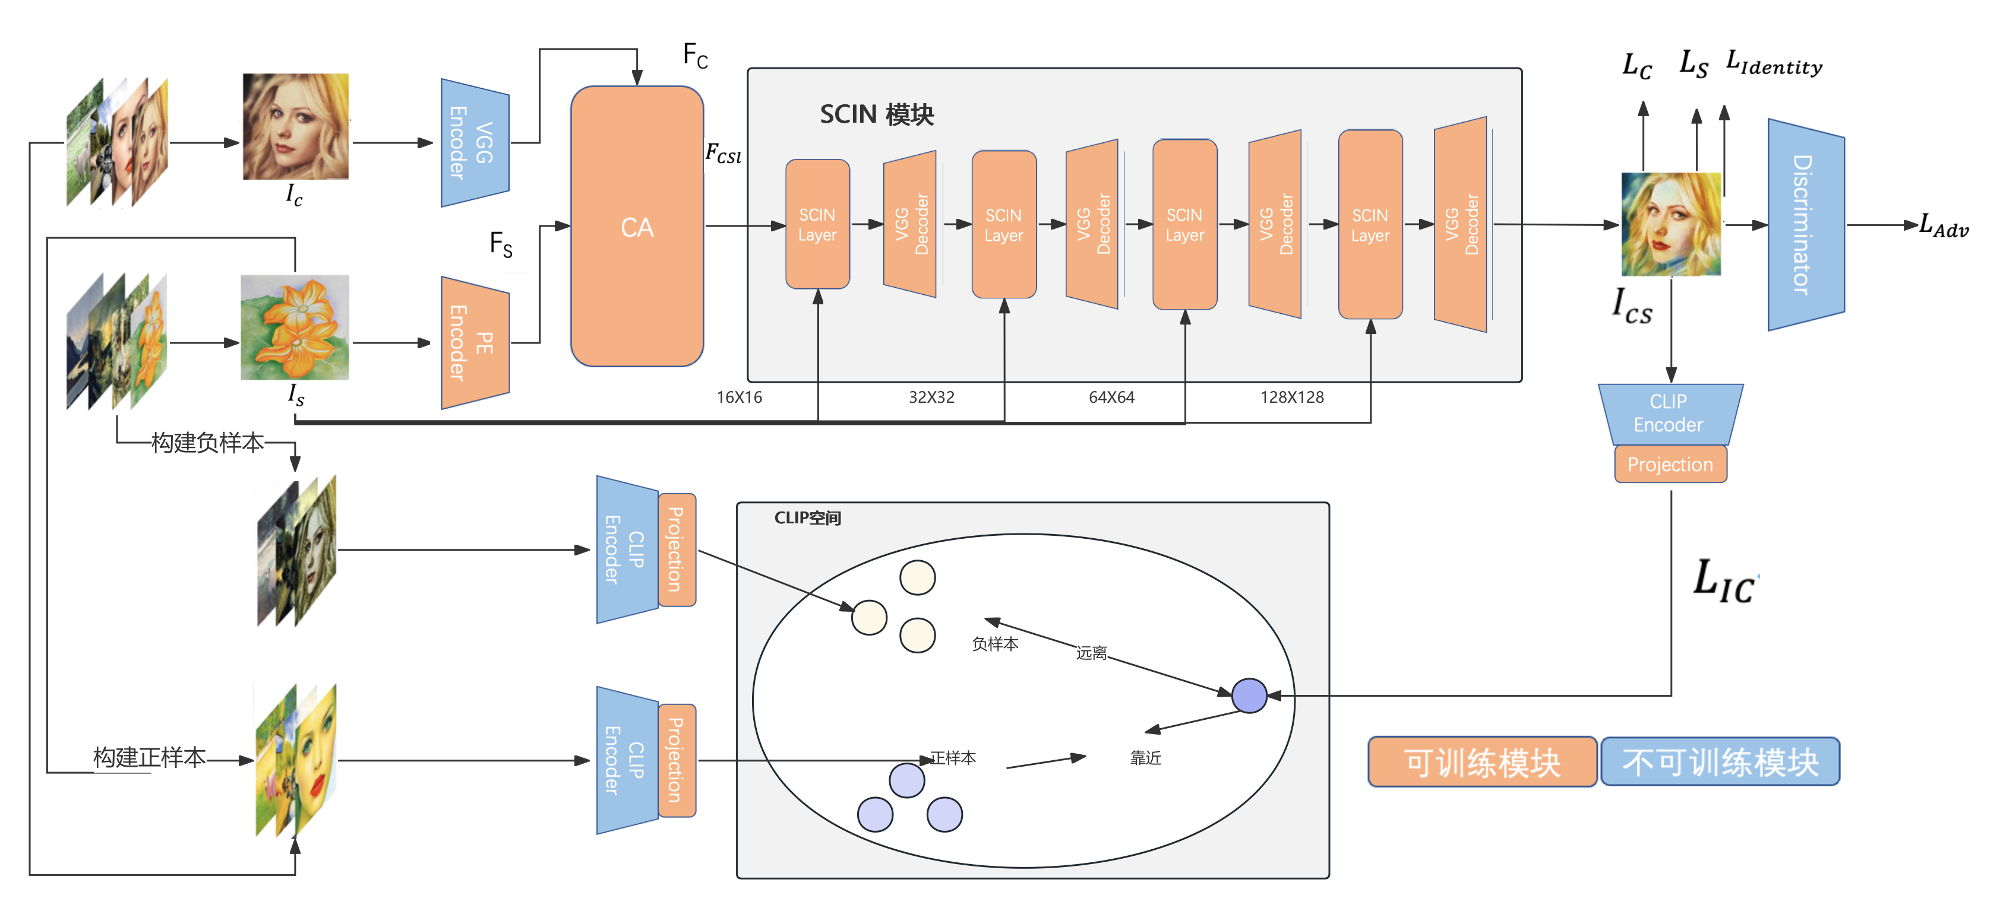
\includegraphics[width=\linewidth]{pics/mainpic2.png}
    \caption{\label{fig:pic_main}方法总览图}
\end{figure}
\subsection{AdaIN方法}
AdaIN~\cite{huang2017arbitrary}提出了自适应实例归一化来对齐内容特征$F_c$的通道均值和方差,以匹配它相应的风格图特征$F_s$。它自适应地从样式输入计算仿射参数,如\autoref{equ:cal_adain}所示:
\begin{equation}
    \label{equ:cal_adain}
    AdaIN(F_c,F_s)=\sigma(F_s)\left(\frac{F_c-\mu(F_c)}{\sigma(F_c)}\right)+\mu(F_s)
\end{equation}
其中 σ(*)和μ(*) 是对输入张量的空间域计算的标准差和均值。给定一个输入批次$x\in R^{N\times C\times H\times W},\mu(x)\text{ 和 }\sigma(x)$可以\autoref{equ:cal_adain_miu_sigma}所示方式计算:
\begin{equation}
    \label{equ:cal_adain_miu_sigma}
    \begin{aligned}
        &\mu_{nc}(x) =\frac1{HW}\sum_{h=1}^H\sum_{w=1}^Wx_{nchw}, \\
        &\sigma_{nc}(x) =\sqrt{\frac1{HW}\sum_{h=1}^H\sum_{w=1}^W\left(x_{nchw}-\mu_{nc}(x)\right)^2+\epsilon} 
        \end{aligned}
\end{equation}
其中$\epsilon$为一个极小量,其主要作用是防止$\sigma_{nc} (x)$为0。
\par 经过这一操作,AdaIN可以快速地的让内容图像同风格图像的全局特征对齐。这一方法在任意风格迁移领域有着很大的影响力。

\subsection{CA模块结构}
本节使用的交叉注意力模块(Cross Attention)目的是根据内容图像的语义空间分布,充分且高效地融合风格图像的局部特征属性。
它通过查询内容特征并在空间上重新排列样式特征来学习内容特征和样式特征之间的局部相关性。其示意如\autoref{fig:pic_ca}所示。
\begin{figure}[htbp]
    \centering
    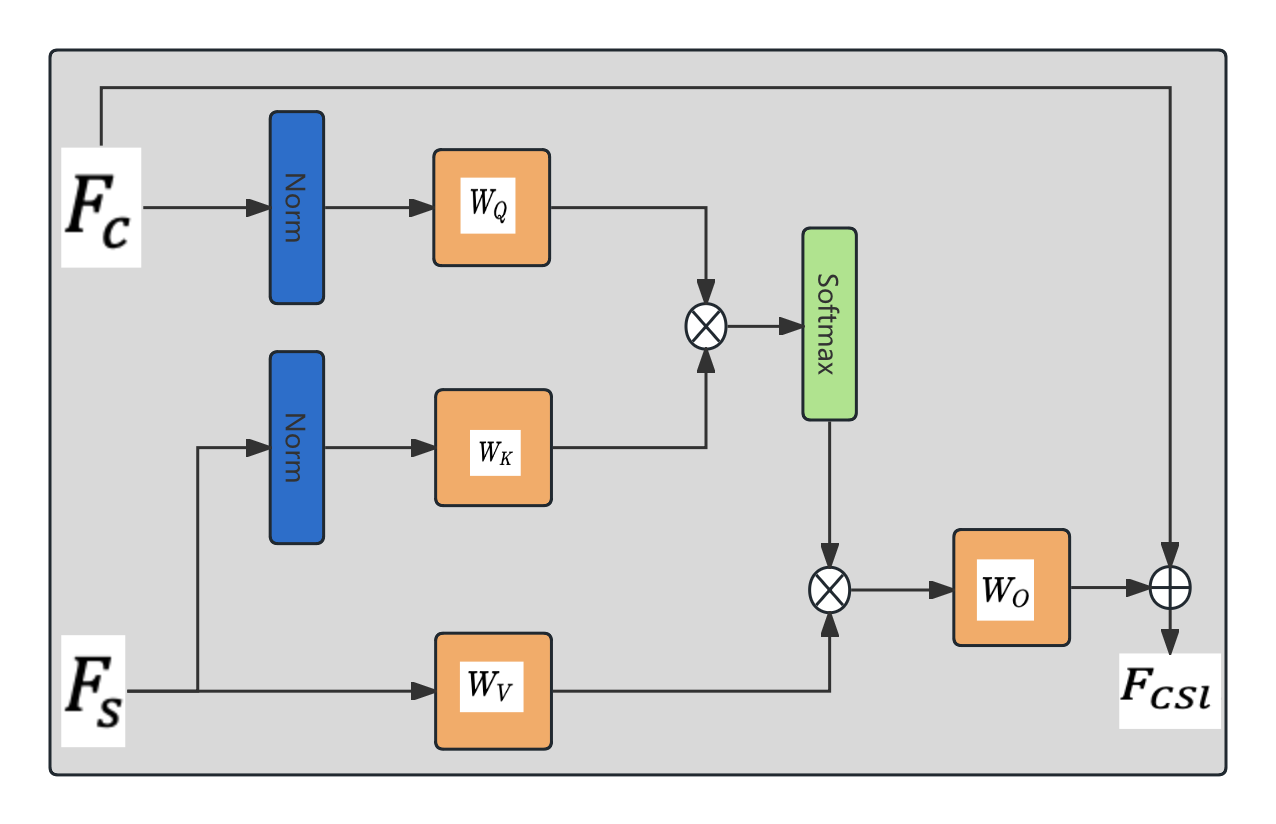
\includegraphics[width=.6\linewidth]{pics/ca.png}
    \caption{\label{fig:pic_ca}交叉注意力模块示意图}
\end{figure}
其计算过程如下述,首先从VGG编码器得到内容图像向量$F_c$,从PE得到风格图像向量$F_s$,然后经过如\autoref{equ:cal_fattn}所示计算得到混合了内容特征与风格局部特征的结果$F_{Attn}$:

\begin{equation}
    \label{equ:cal_fattn}
    F_{Attn}=W_O\cdot(softmax\left(\frac{(W_Q\cdot c_{norm}(F_C))\cdot(W_K\cdot c_{norm}(F_S))^T}{\sqrt{d}}\right)\cdot W_VF_S)
\end{equation}
其中$W_O$、$W_Q$、$W_K$、$W_V$分别是几个可训练的权重矩阵,$c_{norm} (*)$是channel-wise的归一化计算操作,$softmax(*)$是归一化指数函数。
把得到的$F_{Attn}$同原来的$F_C$相加,得到最终结果$F_{CSl}$,如\autoref{equ:cal_fcsl}所示。
\begin{equation}
    \label{equ:cal_fcsl}
    F_{CSl}=F_{Attn}+F_C
\end{equation}

\subsection{SCIN模块的结构}
SCIN模块的目的是学习得风格图像的全局信息特征,并且把它融合到含有内容信息的特征张量中。
它由多个SCIN Layer模块和多个VGG的解码器层串联构成,每个模块接受风格图输入和特征张量输入。
通过多头自注意力机制习得风格图像的全局特征并且将其融合到内容特征中。\autoref{fig:pic_scinlayer}是第i层SCIN layer的结构:

\begin{figure}[htbp]
    \centering
    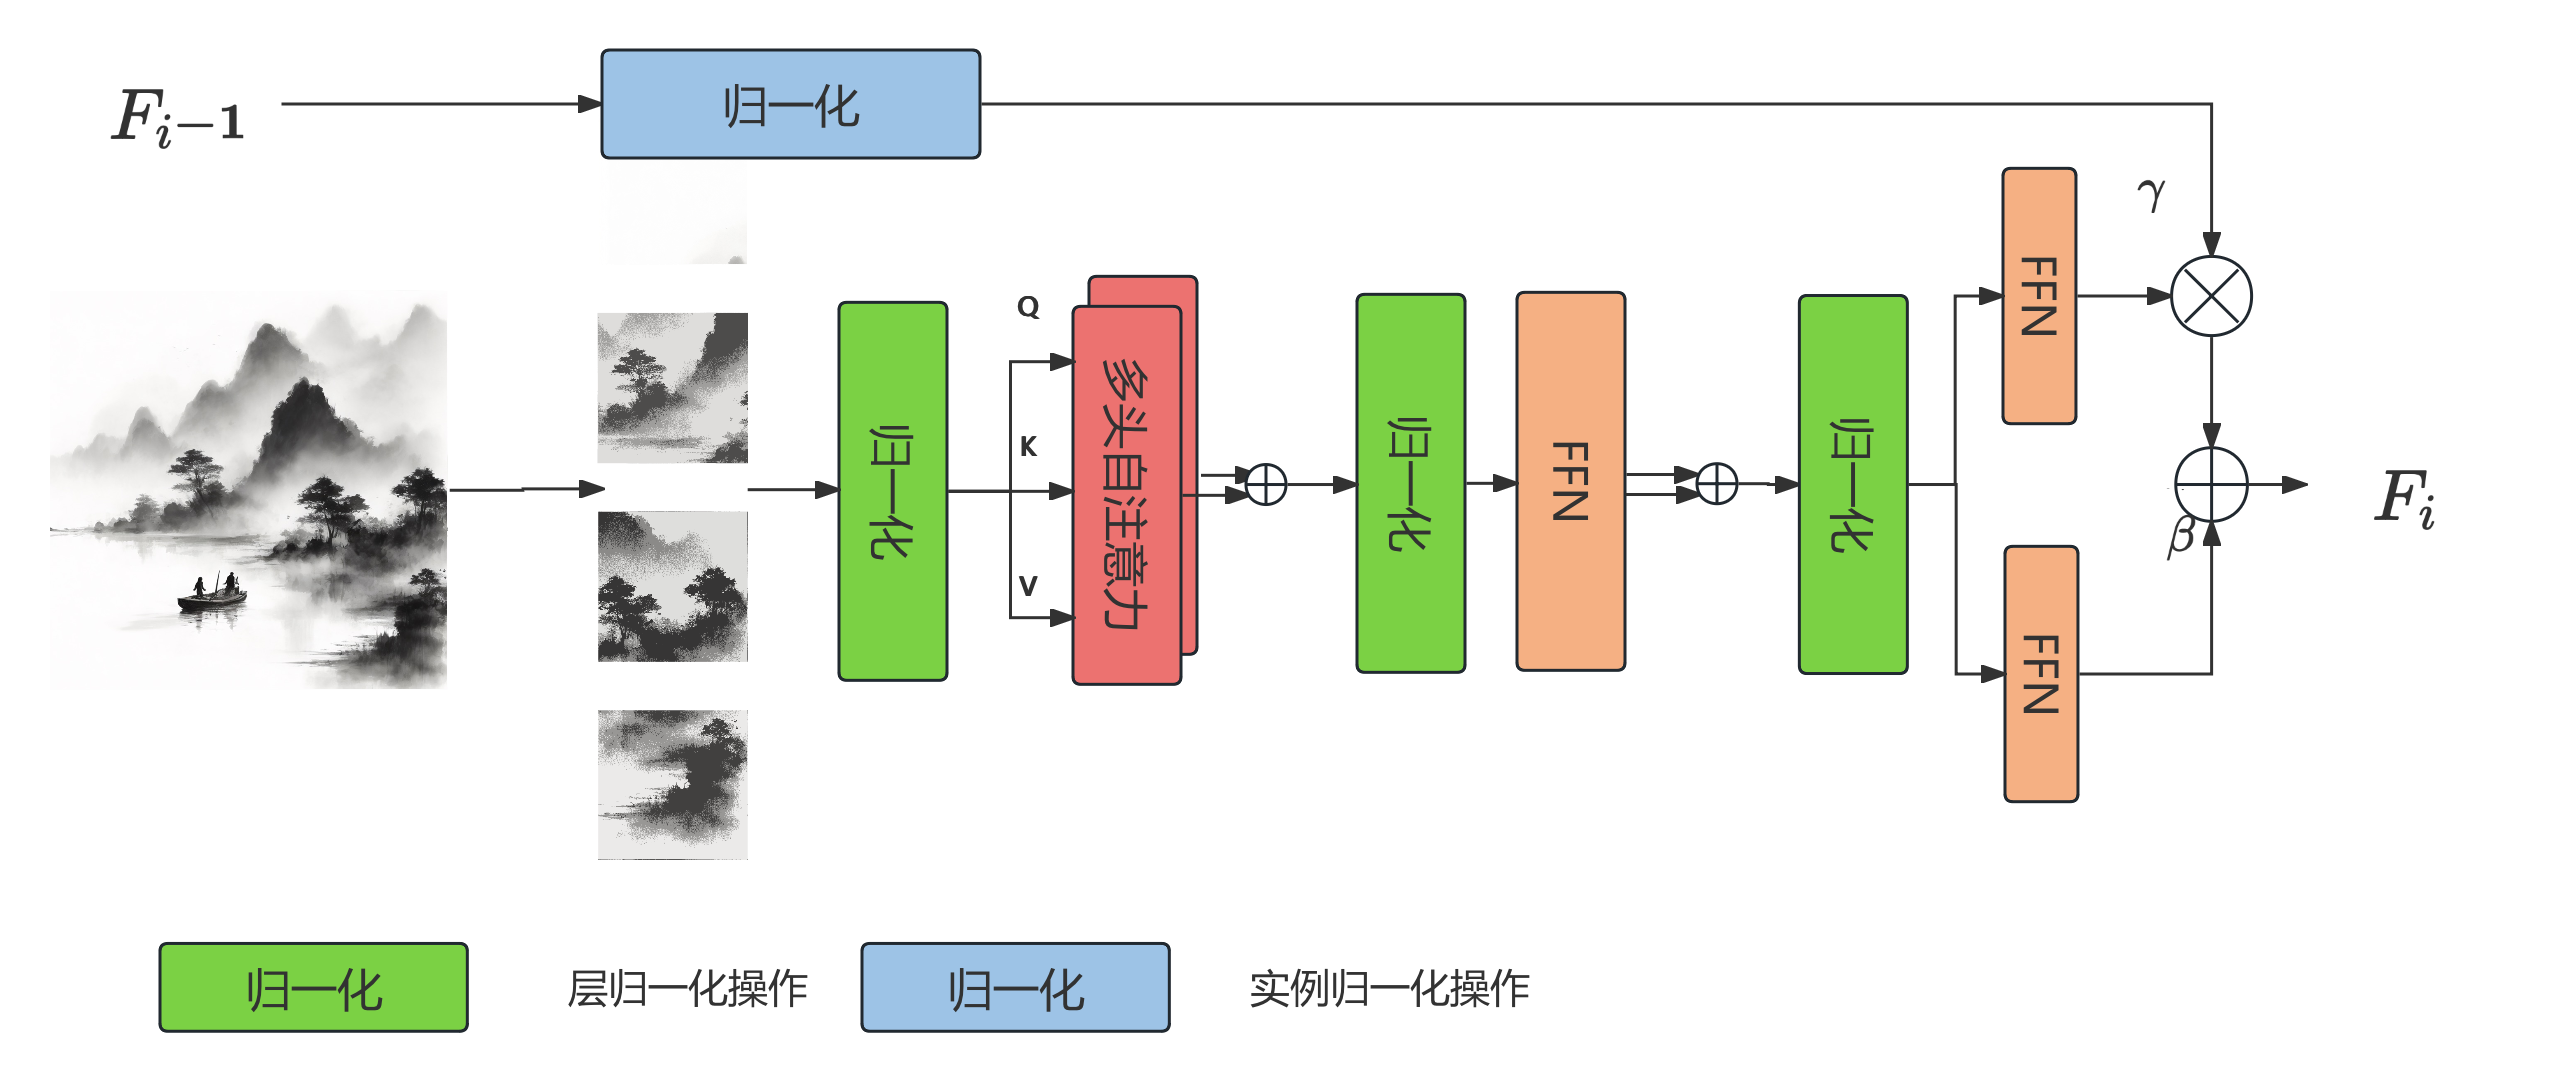
\includegraphics[width=\linewidth]{pics/scinlayer.png}
    \caption{\label{fig:pic_scinlayer}SCIN Layer结构图}
\end{figure}
\autoref{fig:pic_main}中SCIN模块中使用的解码器层是同VGG编码器对应层的镜像结构,并且使用预训练权重初始化。考虑到特征向量每次经过解码器层都会导致其宽高尺寸变大一倍,
本节采用梯次变大的多尺度的风格图片输入以减少计算量。具体来说可以采用如下计算方式进行处理:
\par 对于第i个SCIN Layer,(在本文的实际实验中共有4层,i依次能取1,2,3,4),给定一组输入风格序列的嵌入张量\(Z_{s}^{i}=(E_{s1},E_{s2},\ldots,E_{sn})\),
首先将其输入到transformer的编码器层。输入序列被归一化后,被编码为Q、K和V,如\autoref{equ:cal_scin_qkv}所示:
\begin{equation}
    \label{equ:cal_scin_qkv}
    Q=l_{norm}(Z_{s}^{i}W_{q}),K=l_{norm}(Z_{s}^{i}W_{k}),V=l_{norm}(Z_{s}^{i}W_{v})
\end{equation}
其中\(W_q,W_k,W_v\in\mathbb{R}^{C\times d_{head}},l_{norm}(*)\)是层归一化计算,随后可以用\autoref{equ:cal_scin_msa}计算多头自注意力的值:
\begin{equation}
    \label{equ:cal_scin_msa}
    F_{\mathbf{MSA}}(Q,K,V)=\text{ Concat( Attention }_1(Q,K,V),\ldots,\text{ Attention }_N(Q,K,V))\cdot W_o
\end{equation}
其中$W_o\in\mathbb{R}^{C\times C}$也是可学习的参数, N是多头的个数,\(d_{head}=\frac cN\)是注意力头的维度;
那么可以用\autoref{equ:cal_scin_ysi}计算得到编码的风格序列$Y_s^i$:
\begin{equation}
    \label{equ:cal_scin_ysi}
    \begin{aligned}&Y_s^{\prime}=l_{norm}(F_{\mathrm{MSA}}(Q,K,V)+Z_s^i)\\&Y_s^i=l_{norm}(F_{\mathrm{FFN}}(Y_s^{\prime})+Z_s^i)\end{aligned}
\end{equation}
其中$F_{\mathrm{FFN}}(Y_{s}^{\prime})=\max(0,Y_{s}^{\prime}W_{1}+b_{1})W_{2}+b_{2}$代表一次前馈计算步骤。
在获得了编码的风格序列特征后,参考AdaIN的思路,本章也提出把包含内容风格的特征对齐到$Y_s^i$上,以完成内容特征与全局风格特征的融合。
但是和AdaIN不同的是,本方法中的特征和偏置变量是来源于风格的全局特征的。对于给定的风格序列编码$Y_s^i$分别计算其尺度特征\(\gamma_{s}^{i}\)和偏置特征\(\beta{s}^{i}\),
如\autoref{equ:cal_scin_gamma_beta}所示:
\begin{equation}
    \label{equ:cal_scin_gamma_beta}
    \gamma_s^i=F_{FFN}^i(Y_s^i),\beta_s^i=F_{FFN}^i(Y_s^i)
\end{equation}
具体来说,对于第i个SCIN Layer,记$F_i$为该层的输出,$D_i$为该层SCIN Layer后跟的解码器层, 
$F_{(i-1)}$为其上一层的输出。从$Y_s^i$中抽取特征得到\(\gamma_{s}^{i}\)和\(\beta{s}^{i}\),将这两个特征同上一层SCIN Layer的输出$F_{(i-1)}$相融合,得到输出结果$F_i$。
如\autoref{equ:cal_scin_fi}所示:
\begin{equation}
    \label{equ:cal_scin_fi}
    F_i=\gamma_s^i\otimes\mathrm{IN}(D_i(F_{i-1}))\oplus\beta_s^i
\end{equation}
其中的$\oplus$和$\otimes$运算为逐通道的加法和乘法操作。
特别地,当计算\(D_0(F_0)\)的时候,用\(D_0(F_0)=F_{CSl}\)完成计算,其中$F_{CSl}$为上一小节中获得的特征。
以此计算完四个值可以得到混合了内容特征、全局风格特征和局部风格特征的结果\(SCIN(F_{CSl},Y_S^1,Y_S^2,Y_S^3,Y_S^4)\),它就是\(D_4(F_4)\)。

\subsection{PE模块结构}

由于在之前的风格迁移工作中,大多使用VGG作为风格图像的编码器,其在一些特定的风格风格类型图,如人脸的特征提取时有天然的缺陷,
它会在关注风格特征的同时关注到比如人眼这种结构特征,而这是实际应用中所不需要的。如果采用基于transformer的架构,则它在高频特征提取的工作中表现不佳。
为了解决这一两难问题,受Inception Transformer~\cite{si2022inception}启发,本节提出了一种新的感知编码器(PE),
它可以捕获风格信息,避免过多关注风格图像中的显著分类特征,并在后续的消融实验中中验证了它的优越性。详细架构如\autoref{fig:pic_peblock}所示。
\begin{figure}[h]
    \centering
    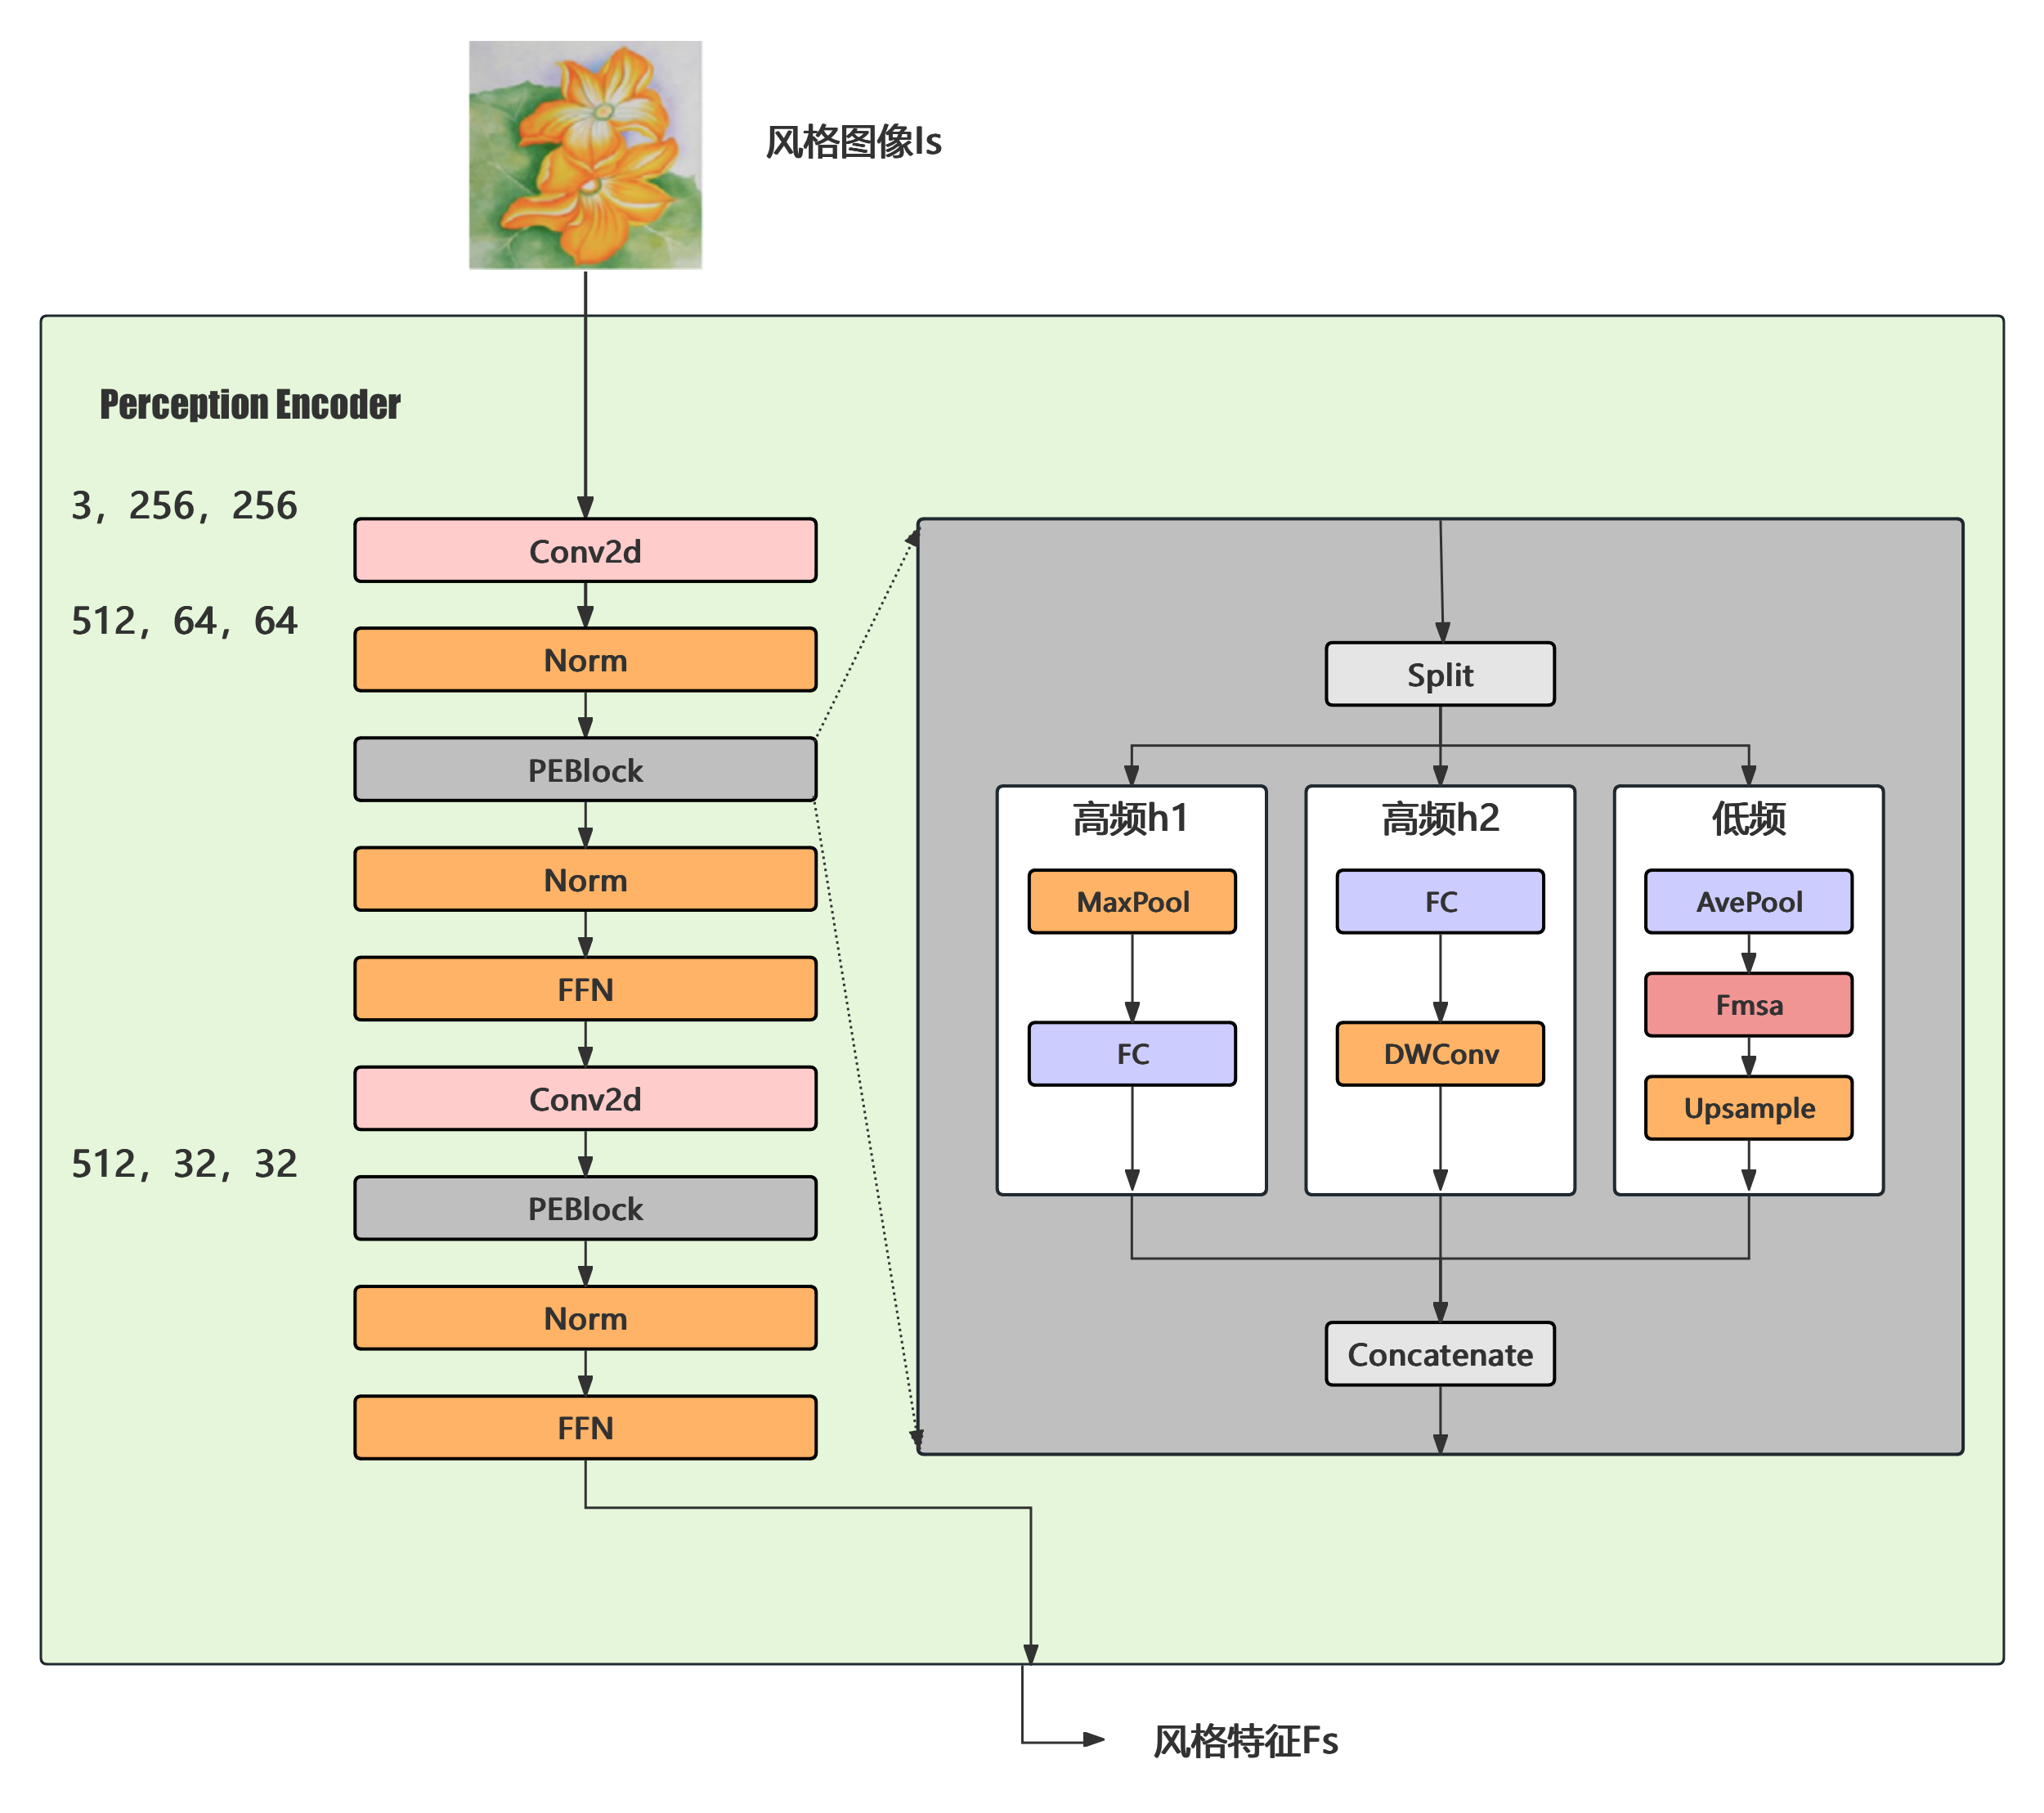
\includegraphics[width=\linewidth]{pics/pe.png}
    \caption{\label{fig:pic_peblock}PE Block的结构图}
\end{figure}
以第一个PE Block的计算为例,向量块\(F_s^{512\times64\times64}\)被输入到PE Block中,
它被沿通道维度均分为高频和低频分量\(F_h^{256\times64\times64}\text{和}F_l^{256\times64\times64}\)。
本节采用了一种并行结构来学习高频分量\(F_{h1}^{128\times64\times64}\text{和}F_{h2}^{128\times64\times64}\)。$F_{h1}$使用最大池化和线性层进行嵌入,~\cite{szegedy2015going}
$F_{h2}$被馈送到线性和深度卷积层~\cite{mamalet2012simplifying,chollet2017xception}。
而$F_l$依次经过平均池化、多头自注意力计算、上采样步骤。此过程可如\autoref{equ:cal_peblock_fl}表达:

\begin{equation}
    \label{equ:cal_peblock_fl}
    \begin{gathered}
        Y_{\boldsymbol{h}1}=\mathrm{FC}(\mathrm{MaxPool}(\boldsymbol{F}_{\boldsymbol{h}1})) \\
        Y_{h2}=\mathrm{DwConv}(\mathrm{FC}(F_{h2})) \\
        \boldsymbol{F}_{l}=\mathrm{Upsample}\left(F_{\mathrm{MSA}}(\mathrm{AvePooling}(\boldsymbol{F}_{l}))\right) \\
        F_{PE Block}=\mathrm{Concat}(Y_l,Y_{h1},Y_{h2})
        \end{gathered}
\end{equation}
输入的风格图像依次经过二维卷积、PEBlock1、下采样、PEBlock2之后,得到风格特征。

\subsection{基于实例的对比学习方法}
对比学习已被用于许多领域~\cite{chen2020improved,han2021dual,wu2021contrastive},该方法已经被证明可以保留内容图像的内容~\cite{han2021dual}并增强风格化图像的风格~\cite{chen2021artistic}。
为了更好地去除风格化的伪影、提升风格化的质量,本节提出了一种新的 ICL 来学习风格化到风格化的关系。
考虑到VGG网络是在规模较小的ImageNet数据集(约1400万个图像样本)上进行的训练,而CLIP模型~\cite{radford2021learning}是在更大的数据集上进行的训练,
本节没有使用以前基于VGG的对比学习~\cite{han2021dual},而是利用预训练的CLIP模型的图像编码器来获得基于实例的潜在代码空间,
以更好地衡量图片的相似程度、优化风格化到风格化的关系。CLIP是一个大型的多模态预训练神经网络,
由OpenAI在2021年发布。‌该模型基于对比学习的原理,通过大量图像和文本的配对数据(约4亿个文本-图像对)进行预训练,
学习图像和文本之间的对齐关系,具有多模态学习的能力。CLIP模型由图像编码器和文本编码器两部分组成,
图像编码器可以将图像转换为特征向量,而文本编码器则将文本转换为特征向量。这两个特征向量同属一个向量空间。

\par 基于上述分析,本节实现了基于实例的对比学习,其根据图像的CLIP空间编码来约束图像的像素级表现。其示意图如\autoref{fig:pic_icl}所示。其中蓝色层代表不可训练的网络,橙色层代表可训练的网络。

\begin{figure}[htbp]
    \centering
    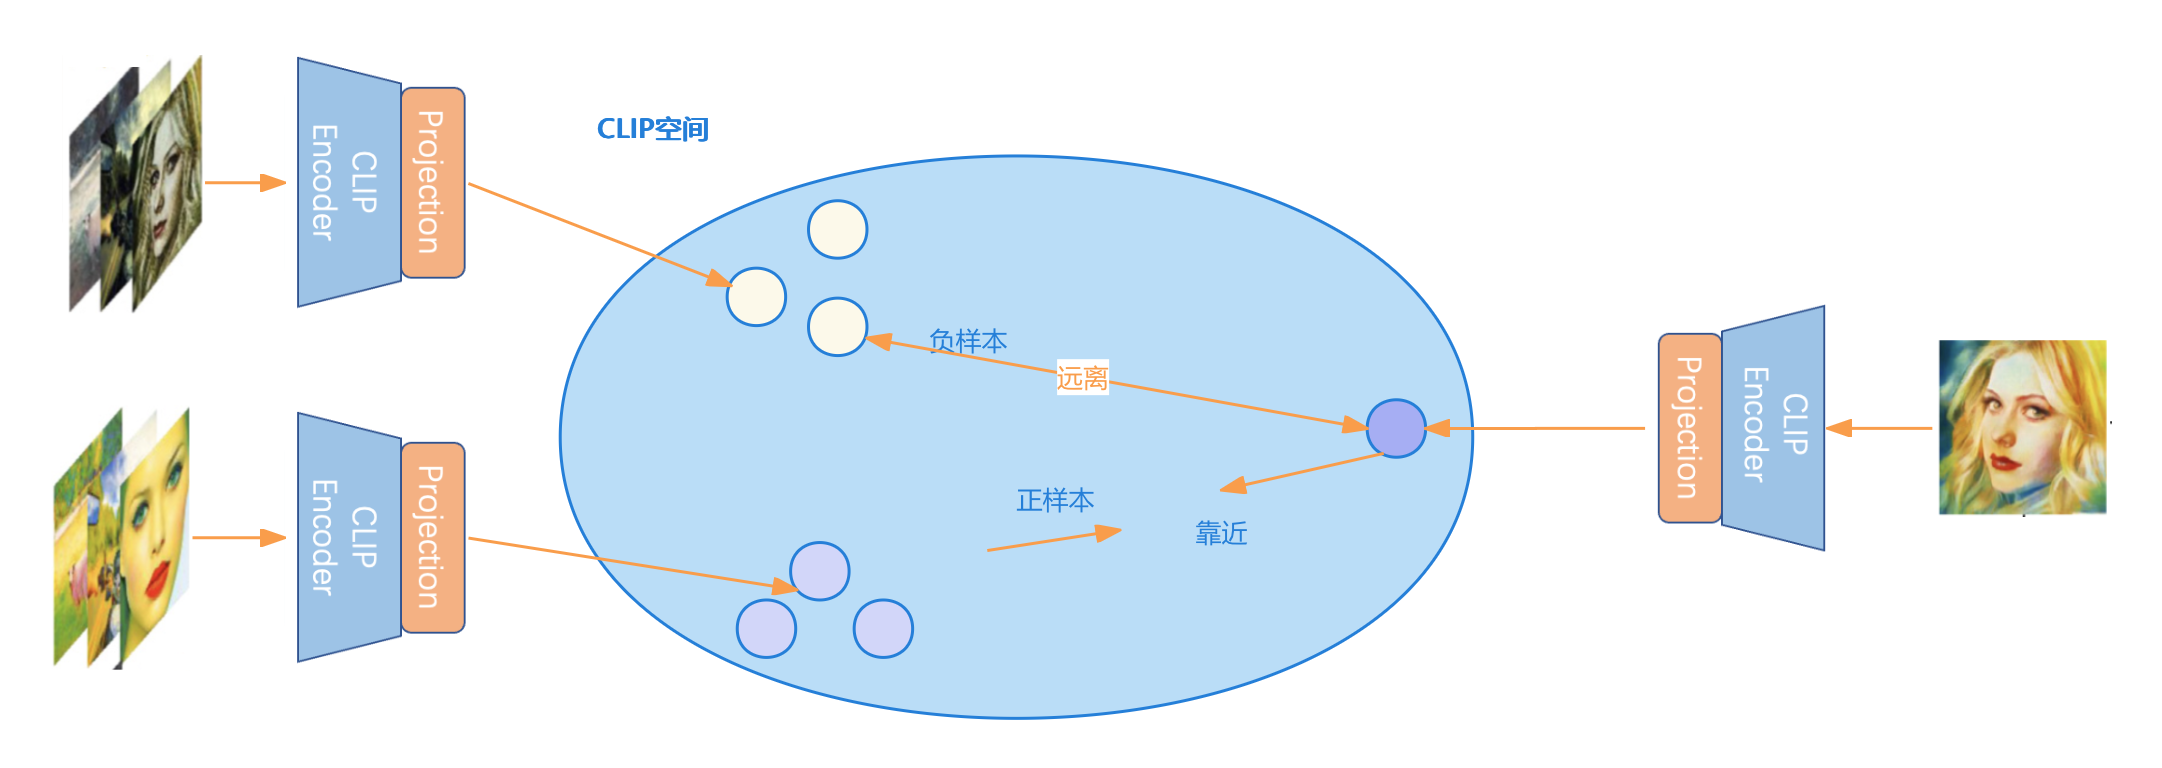
\includegraphics[width=\linewidth]{pics/icl.png}
    \caption{\label{fig:pic_icl}对比学习示意图}
\end{figure}
假设$b_s^n$和$b_c^n$表示样式一批次大小为偶数n的风格图像和内容图像集。对于$b_s^n$和$b_c^n$的每个样式图像$s_j$和内容图像$c_i$,
其中i,j满足\(i\in[0,n-1],j\in[0,n-1]\),并且使用$s_ic_j$来表示这两图像$c_i$、$s_j$的风格化结果。
对于所有内容图像和样式图像,依次构建风格化图像并记为\(S_1C_1,S_1C_2,\ldots,S_1C_n;\ldots,S_nC_1,S_nC_2,\ldots,S_nC_n\);
对于每一个特定的风格化图像$s_i c_j$,按照如下方式构建正负用例:对于全部的定义域内的p和q,当满足$p= i,q\neq j$时,其对应的风格化结果$s_p c_q$被视为$s_i c_j$的正例对,
其含义为同一风格图像进行的全部风格化结果应该是更“相似”的;而当$p\neq i,q\neq j$的时候,其对应的风格化结果$s_p c_q$被视为$s_i c_j$的负例对。
基于这些条件,可以通过\autoref{equ:cal_lic}计算对比学习的损失函数:
\begin{equation}
    \label{equ:cal_lic}
    \begin{gathered}
        L_{IC}=L_{pos}+L_{neg}, \\
        L_{pos} =-log(\frac{P_s}{P_s+N_s}),L_{neg}=-log(\frac{P_c}{P_c+N_c}), \\
        P_s=\exp\left((M_s(s_ic_j)^\top M_s(s_ic_j)/\tau\right), \\
        N_s=\sum exp(M_s(s_ic_j)^\top M_s(s_ic_j)/\tau), \\
        P_c=\exp{(M_c(s_ic_j)^\top M_c(s_ic_j)/\tau)}, \\
        N_c=\sum exp(M_c(s_ic_j)^\top M_c(s_ic_j)/\tau), 
        \end{gathered}
\end{equation}
其中,\(M_s=l_s(E_{clip}(\cdot)),M_c=l_c(E_{clip}(\cdot)),E_{clip}(\cdot)\)代表CLIP模型的图像编码器,
$l_c$和$l_s$是获取内容编码和风格编码的可学习投影网络,如下图所示;$\tau$是控制靠近和远离程度的超参数,设置为0.3。
可以认为,在使用$L_{IC}$约束对projection层进行充分的训练以后,它可以很好地学习到把风格按照本节所提出的规则投影到CLIP空间。

\subsection{损失函数}
本章采用多种损失函数来约束网络的训练,具体包括:感知内容损失$L_C$、感知风格损失$L_S$、对抗损失$L_{Adv}$、
身份损失$L_{Identity}$和实例对比损失$L_{IC}$,下面将具体的对这几个损失进行介绍。
\paragraph{感知内容和风格损失}
\par 按照之前的风格迁移方法~\cite{han2021dual}所述,对于VGG编码器的第x层,记为$E_{VGG}^x$,感知内容和样式损失可以用\autoref{equ:cal_perceptual_loss_cs}计算。

\begin{equation}
    \label{equ:cal_perceptual_loss_cs}
    \begin{gathered}
        L_{C} = \sum_{i=4}^{L} \parallel E_{VGG}^{x}(I_{CS}) - E_{VGG}^{x}(I_{C}) \parallel_{2} \\
        L_{S} = \sum_{i=1}^{L} \parallel \mu(E_{VGG}^{x}(I_{cs})) - \mu(E_{VGG}^{x}(I_{S})) \parallel_{2} + \parallel \theta(E_{VGG}^{x}(I_{CS})) - \theta(E_{VGG}^{x}(I_{S})) \parallel_{2}
    \end{gathered}
\end{equation}
其中$\mu$和$\theta$表示通道上的均值和标准差。对于x的取值,遵照Park等人的设定~\cite{park2019arbitrary},使用了$ReLU4\_1$和$ReLU5\_1$两个层来计算$L_C$,
使用$ReLU1\_1$, $ReLU2\_1$,$ReLU3\_1$,$ReLU4\_1$
和$ReLU5\_1$这五个层来计算$L_S$,以求模型能更加关注不同尺度的风格特征信息。

\paragraph{对抗损失}
\par 本文也使用了生成对抗网络GAN~\cite{goodfellow2020generative}的思想从风格数据集S中学习人类感知的风格信息。
GAN 是一个流行的生成模型,由两个网络(即生成器 G 和鉴别器 D)组成,它们相互竞争以达到纳什均衡。
具体来说,将生成器产生的风格化图像和从S采样的艺术品分别输入到鉴别器中作为虚假数据和真实数据。
在训练过程中,生成器将通过生成逼真的艺术图像来试图欺骗鉴别器,而鉴别器将尝试区分生成的假艺术图像和真实艺术图像。
经过充分的训练,理想状态下,生成器将变得足够强大,可以生成人类感知中足够真实的风格图像。
令$I_{cs}$表示风格化结果,$I_s$表示风格图,$D_s (*)$表示鉴别器的输出。此处的训练目标是让生成器产生的风格化结果尽可能地像真实的风格化作品。
对抗训练损失可以表述为\autoref{equ:cal_ladv}:

\begin{equation}
    \label{equ:cal_ladv}
    \begin{aligned}
    L_{Adv}=E_{y\sim I_s}[\log(D_s(y))]+E_{x\sim I_{cs}}[\log(1-D_s(x)]]
    \end{aligned}
\end{equation}
% \par 如\autoref{alg:sample},这是一个算法
\paragraph{身份损失}
基于注意力的风格迁移往往会丢失内容结构,因此前人提出使用身份损失~\cite{zhao2020unpaired}来解决这个问题。
本章中的$L_{Identity}$可以用\autoref{equ:cal_lidentity}计算:
\begin{equation}
    \label{equ:cal_lidentity}
    \begin{aligned}
        L_{Identity}& =\lambda_{identity1}(\parallel I_{cs}-I_c\parallel_2+\parallel I_{cs}-I_s\parallel_2), \\
        &+\sum_{i=0}^L\lambda_{identity2}(\parallel E_{VGG}^x(I_{cs})-E_{VGG}^x(I_c)\parallel_2 \\
        &+\parallel E_{VGG}^x(I_{cs})-E_{VGG}^x(I_s)\parallel_2),
        \end{aligned}
\end{equation}
其中x可取$ReLU1\_1$, $ReLU2\_1$,$ReLU3\_1$,$ReLU4\_1$
和$ReLU5\_1$,两个$\lambda_{identity}$是与不同损失项相关的权重控制参数。



\paragraph{实例对比损失}
本章提出的ICL模块,经过训练后可以很好地把风格遵照所提出的规则投影到CLIP空间。
训练期间,对于生成的风格化图像,都输入到预训练的CLIP图像编码器和两个可训练的投影层中,
计算出这一个批次输出的风格化损失,为前述模块提供一个风格化到风格化关系的指引。在文中用$L_{IC}$表示这一损失。
\paragraph{总损失}
对上述所有损失进行加权求和,获得最终的目标损失函数$L_{Total}$:\(L_{Total}= \lambda_{1}L_{S}+\lambda_{2}L_{C}+\lambda_{3}L_{Identity}+\lambda_{4}L_{Adv}+\lambda_{5}L_{IC}\)
其中$\lambda_1$、$\lambda_2$、$\lambda_3$、$\lambda_4$、$\lambda_5$是五个权重参数。

\section{实验设计和参数设定}
\subsection{实验环境配置}
本算法基于Python语言和Pytorch~\cite{paszke2019pytorch}深度学习框架实现,实验环境中的硬件配置信息和软件版本信息如\autoref{tab:tab_hardware}和\autoref{tab:tab_software}所示。


%改表格左右竖线可以再tabularx改,然后横线就看加不加hline

\begin{table}[htbp]
    \caption{\label{tab:tab_hardware}硬件配置信息}
    \begin{tabularx}{\linewidth}{c|X<{\centering}}
        \hline
        硬件 & 信息 \\ \hline
        架构 & X86\_64 \\ \hline
        CPU & Intel 酷睿12th Gen Intel(R) Core(TM) i7-12700F \\ \hline
        GPU & NVIDIA GeForce RTX 3090,24GB \\ \hline
        内存 & 512GB \\ \hline
    \end{tabularx}
\end{table}
\begin{table}[htbp]
    \caption{\label{tab:tab_software}第三章实现的软件配置信息}
    \begin{tabularx}{\linewidth}{c|X<{\centering}}
        \hline
        操作系统 & Linux 6.5.0-35-generic \#35~22.04.1-Ubuntu \\ \hline
        NVIDIA驱动 & 535.171.04 \\ \hline
        CUDA & V11.8.89 \\ \hline
        Python & 3.8.3 \\ \hline
        PyTorch & 1.13.1+cu116 \\ \hline
    \end{tabularx}
\end{table}
\subsection{实验设置}
本章所述的模型分训练阶段和推理阶段。准备阶段,把所有的数据集的图像都调整大小到512 $\times$  512 像素;训练阶段所有图像都被裁剪为256 $\times$ 256 像素。
其模型中的GAN鉴别器采用和~\cite{wang2018high}一致的多尺度鉴别器设置。
ICL模块中的投影层是一个两层 MLP,每层有 128 个单元。训练的时候使用鉴别器和ICL模块参与。
本章采用学习率为0.0001的Adam优化器~\cite{diederik2014adam}进行训练,批次大小设置为16,训练轮次为160000。
使用的超参数设定为$\lambda_1=1$、$\lambda_2  =1$、$\lambda_3=5$、$\lambda_4=1$、$\lambda_5=0.3$ ,$\tau=0.3$,$\lambda_{identity1}=50$,$\lambda_{identity2}=1$。
\par 在推理阶段,网络已经具有了充分的风格迁移功能,不再需要鉴别器和ICL模块的参与。
另外,在推理测试的时候,使用了随机收集的一些风格图片,包括油画、水彩画、草图等。此外,还使用了一些其他的图片,
包括建筑物、森林和活照片,作为内容图像,并保持其原始大小被馈送到本章所提出的模型以生成风格化图像。

\subsection{实验数据集}
本章实验所采用的的内容图和风格图全都来自MS-COCO数据集~\cite{lin2014microsoft}和WikiArt数据集~\cite{wikiart2018}。
\paragraph{MS-COCO数据集}
COCO(Common Objects in Context)数据集是一个由微软公司创建的、由来自 Google、加州理工学院和佐治亚理工学院等众多知名机构的计算机视觉专业人士维护的合作项目。其用于对象检测、分割和字幕任务的大规模图像识别数据集。它包含超过330,000 张图像,包含来自 80 多个生活中常见的物体和 91 个通用类别的图像,这意味着该数据集可以比小规模数据集更有效地用于对通用模型进行基准测试。COCO 数据集广泛用于计算机视觉研究,并已用于训练和评估许多最先进的对象检测和分割模型。数据集主要有两个部分:图像及其注释。其中图像被组织成一个目录层次结构,顶级目录包含训练、验证和测试集的子目录;注释以 JSON 格式提供,每个文件对应一张图片。数据集中的每个注释都包含图像文件名、尺寸、以及用于目标检测的标注等信息。本章中主要使用图像数据进行训练。
\paragraph{WikiArt 数据集}
WikiArt数据集由WikiArt组织创建和维护。它包含来自 195 位不同艺术家的画作。该数据集有 42129 张用于训练的图像和 10628 张用于测试的图像。它具有完善的结构,因此经常被用于艺术生成的机器学习领域。本章主要使用其图像充当风格图像用于训练。

\subsection{评价指标}
本节将从主观和客观指标两个方面对结果进行评估。主观方面,本节中使用欺骗分数(DS)进行测评:
作者为每个方法随机选择 20 张合成图像,并邀请了50名受试者参与测评。
为了更直观地比较本章所提出的方法的优势,随机选择相同数量的WikiArt图像来询问这50个受试人。
客观方面,本节将从内容保真程度和人眼感知的两个角度对工作效果进行客观的量化评估。
遵循在本文第2.4节描述的评价指标,对本文的评估采用内容保真度(Content Fidelity,CF), 
全局影响分数(Global Effects ,GE)和本地图样分数(Local Patterns ,LP)~\cite{wang2021evaluate}指标,
保证指标覆盖了感知和风格化表现这两个方面。其中CF量化计算内容的保护程度,而为了计算方便,本节决定采用GE+LP来衡量对于人眼的感知优劣。

\section{实验结果和分析}
在本节中,首先展示本章所提出的方法在数据集上进行实验后获得的风格迁移结果,然后展示本算法与近年来表现较好的一些二维任意风格迁移算法之间的效果对比,包括定性对比与定量对比,最后对本算法中提出的几个创新模块进行消融实验以验证每个模块的有效性。
\subsection{结果展示}
在本小节中,随机选择了一些风格图和内容图进行了实验得到了一些风格化图像,并将其展示在\autoref{fig:pic_direct_show_3_1}和\autoref{fig:pic_direct_show_3_2}中。每个图的第一行、第二行、第三行分别为风格图、内容图和风格化图。从中可以看出本章提出的方法对于各种风格都有着较好的风格化能力,其风格化结果存在较少的伪影,没有人眼等显著的实物特征,并且风格图和风格化结果之间具有相应的笔触、线条等风格特征。

\begin{figure}[htbp]
    \centering
    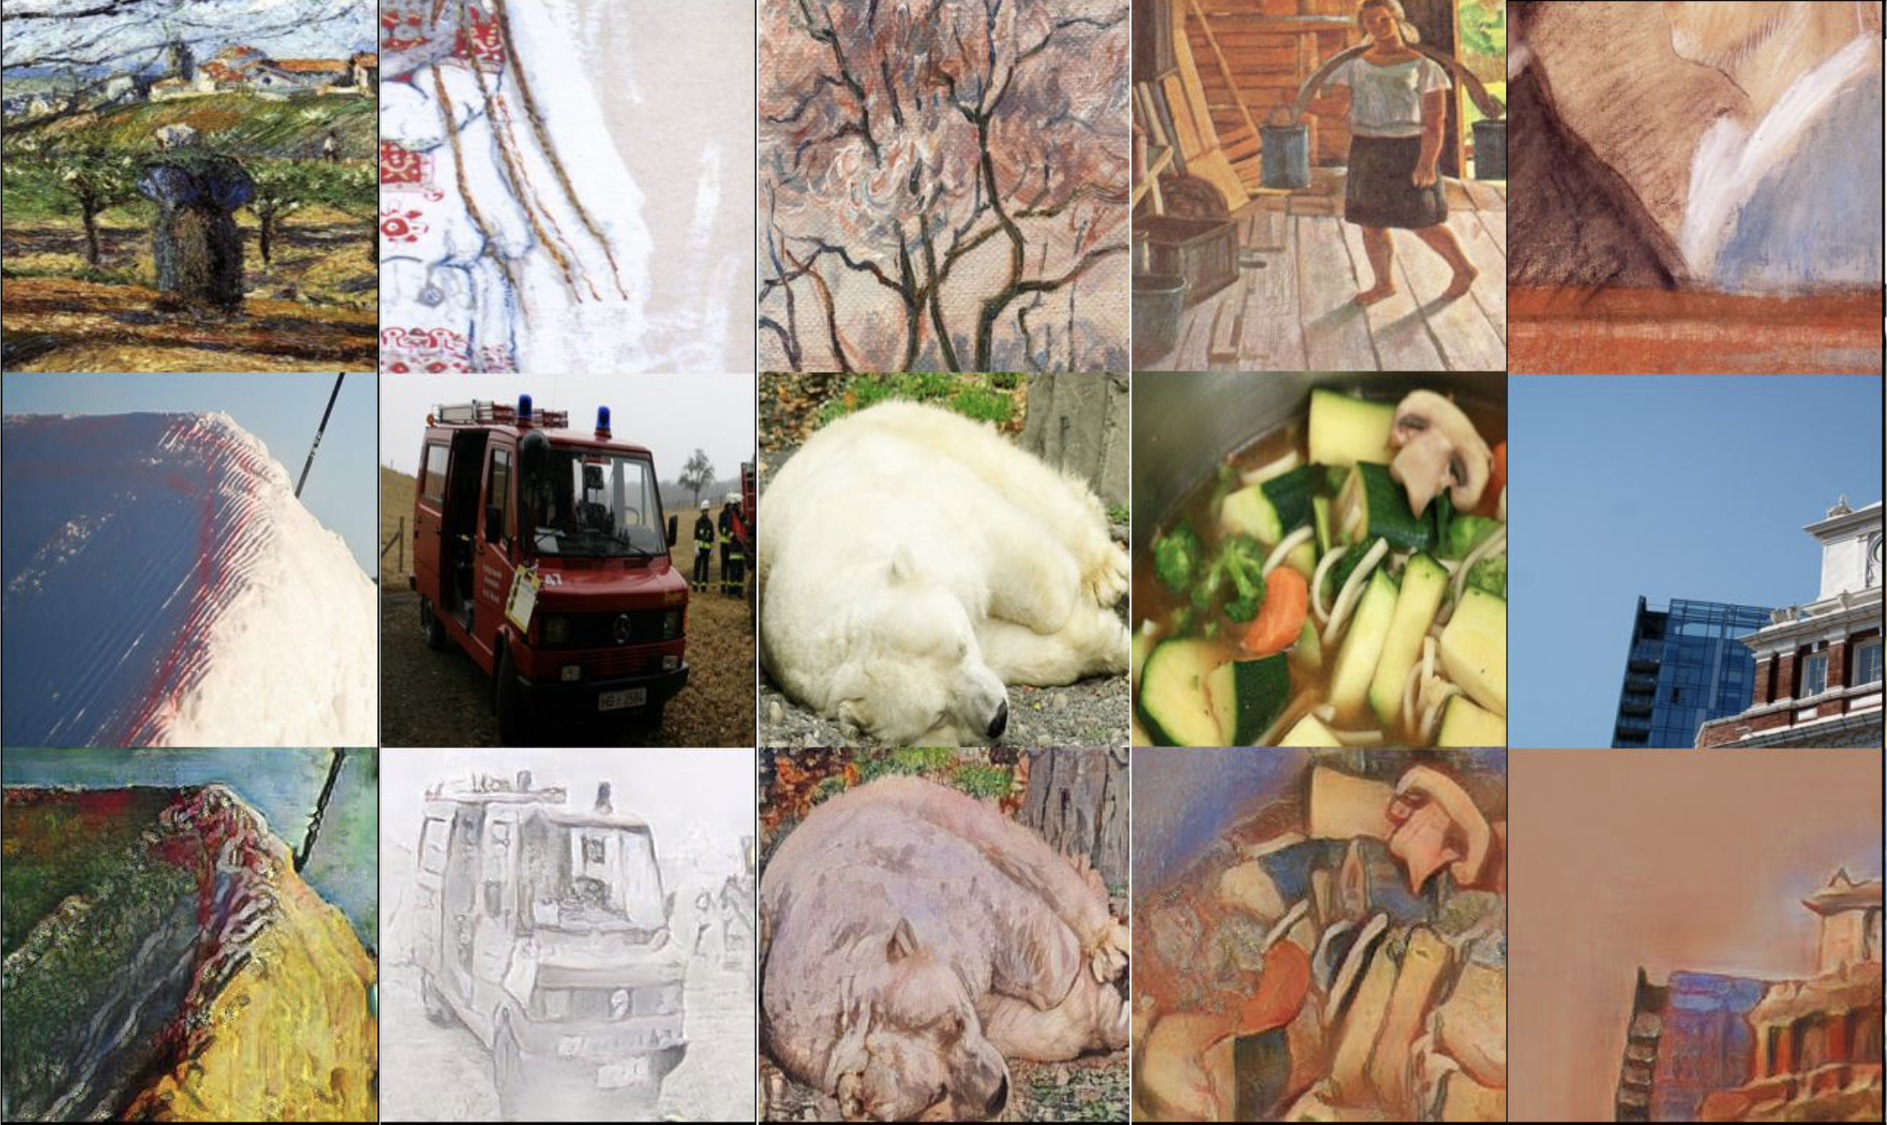
\includegraphics[width=\linewidth]{pics/showres_direct3.1.png}
    \caption{\label{fig:pic_direct_show_3_1}风格化结果展示图1}
\end{figure}
\begin{figure}[htbp]
    \centering
    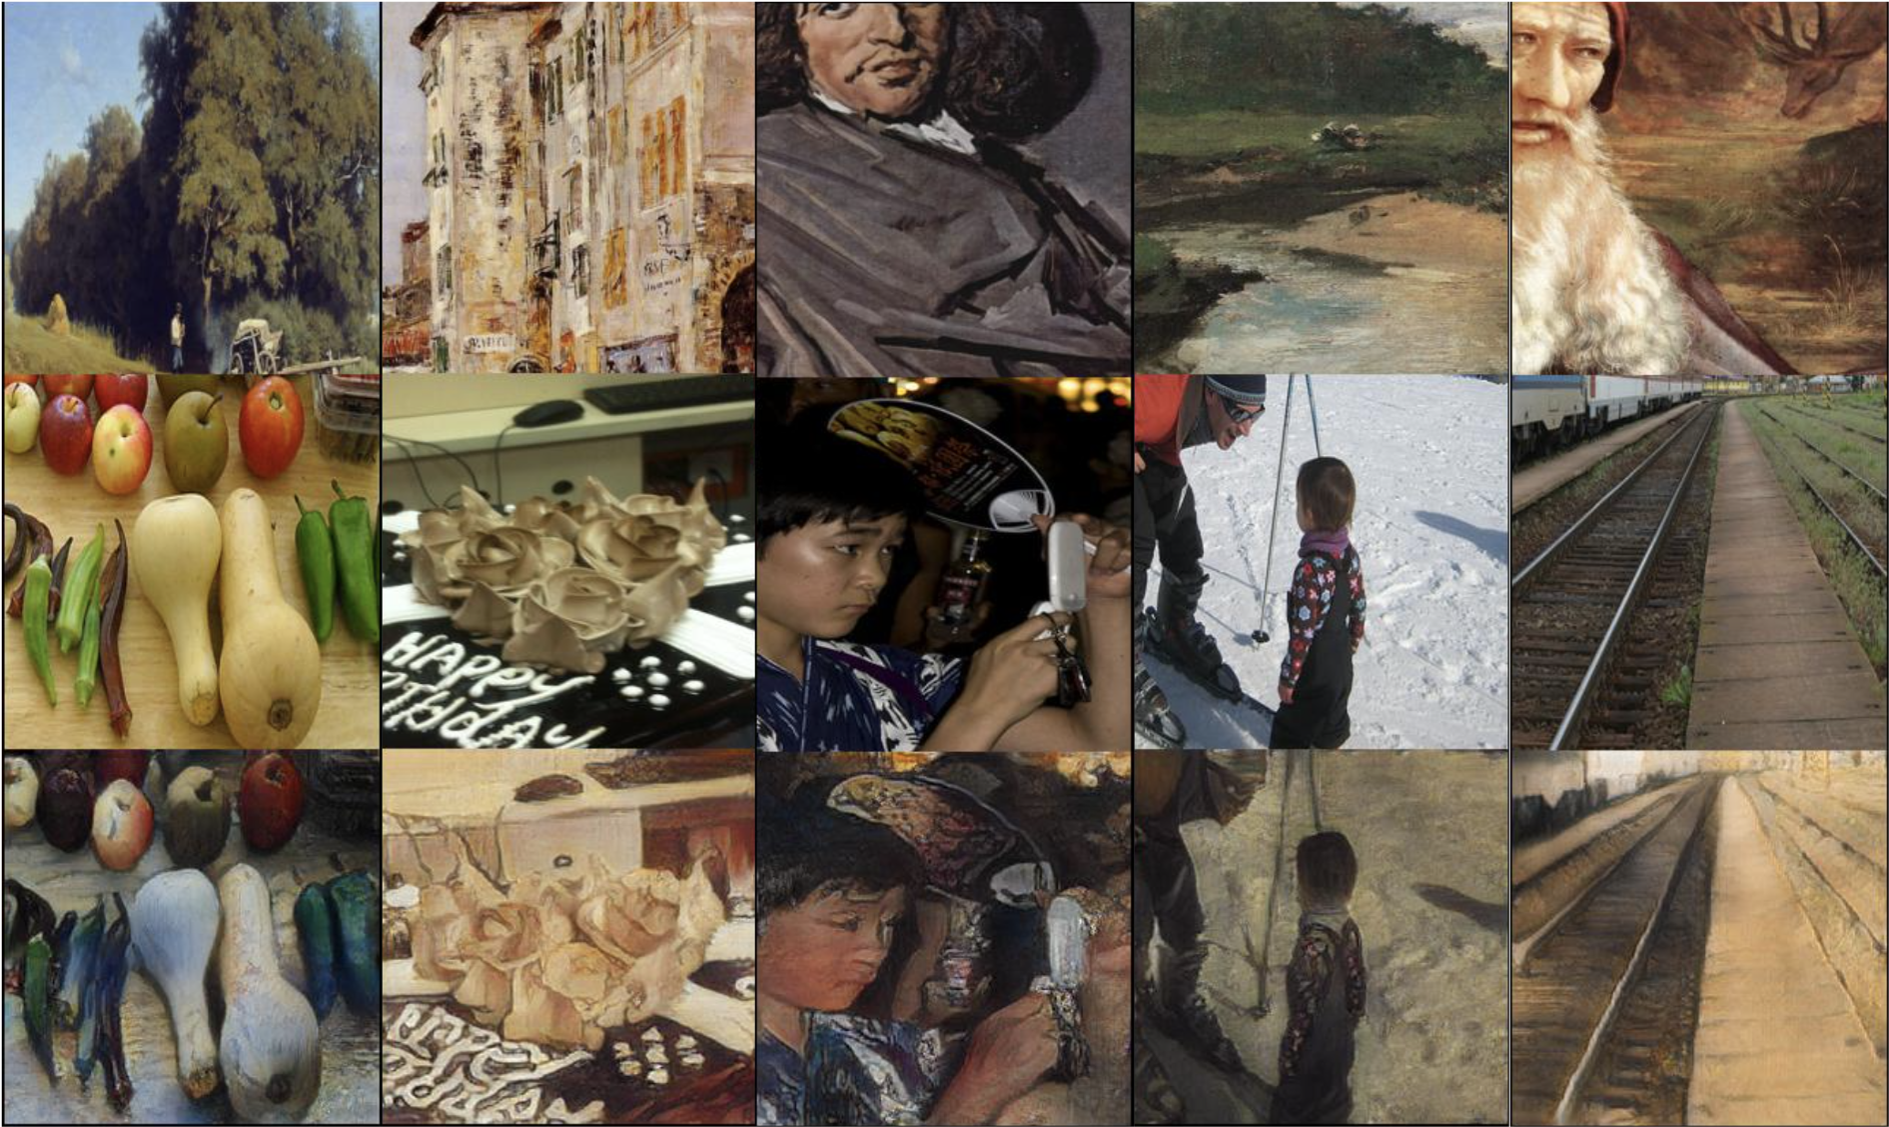
\includegraphics[width=\linewidth]{pics/showres_direct3.2.png}
    \caption{\label{fig:pic_direct_show_3_2}风格化结果展示图2}
\end{figure}
\subsection{对比试验和分析}
\paragraph{定性实验对比和分析}
将本章所提出的方法与最先进的方法进行比较,包括基于注意力的风格迁移:IEAST~\cite{chen2021artistic}、AdaAttn~\cite{liu2021adaattn}、
MAST~\cite{deng2020arbitrary}、SANet~\cite{park2019arbitrary}、AesUst~\cite{wang2022aesust}、SttyTr2~\cite{deng2022stytr2}、
非基于注意力的风格迁移:AdaIN~\cite{huang2017arbitrary}、DEAST~\cite{zhang2022domain}、WCT~\cite{li2017universal}、ArtFlow~\cite{an2021artflow}、
LST~\cite{li2019learning}、AST~\cite{hu2020aesthetic}、CCPL~\cite{wu2022ccpl}。比较的结果如\autoref{fig:pic_compare_3_1}和\autoref{fig:pic_compare_3_2}所示。
IEAST、AdaAttN、MAST、SANet 和 AesUST 有时会从样式图像引入不希望的语义结构到风格化结果。
WCT 在内容保存方面存在严重的问题。AdaIN存在内容结构模糊和样式模式失真问题。StyTr2、DEAST、ArtFlow 和 LST 无法从样式图像中学习局部纹理。
虽然 CCPL 可以有效地保持内容结构,但它的结果中颜色分布较为混乱和无序,下图中粉色的区域无法判断语义信息。
对于 AAST,风格图像和风格化图像之间存在明显的风格偏差。与这些方法相比,本章提出的方法可以生成具有内容结构和风格纹理的风格化图像,并且不引入无法解释的语义结构。
\begin{figure}[htbp]
    \centering
    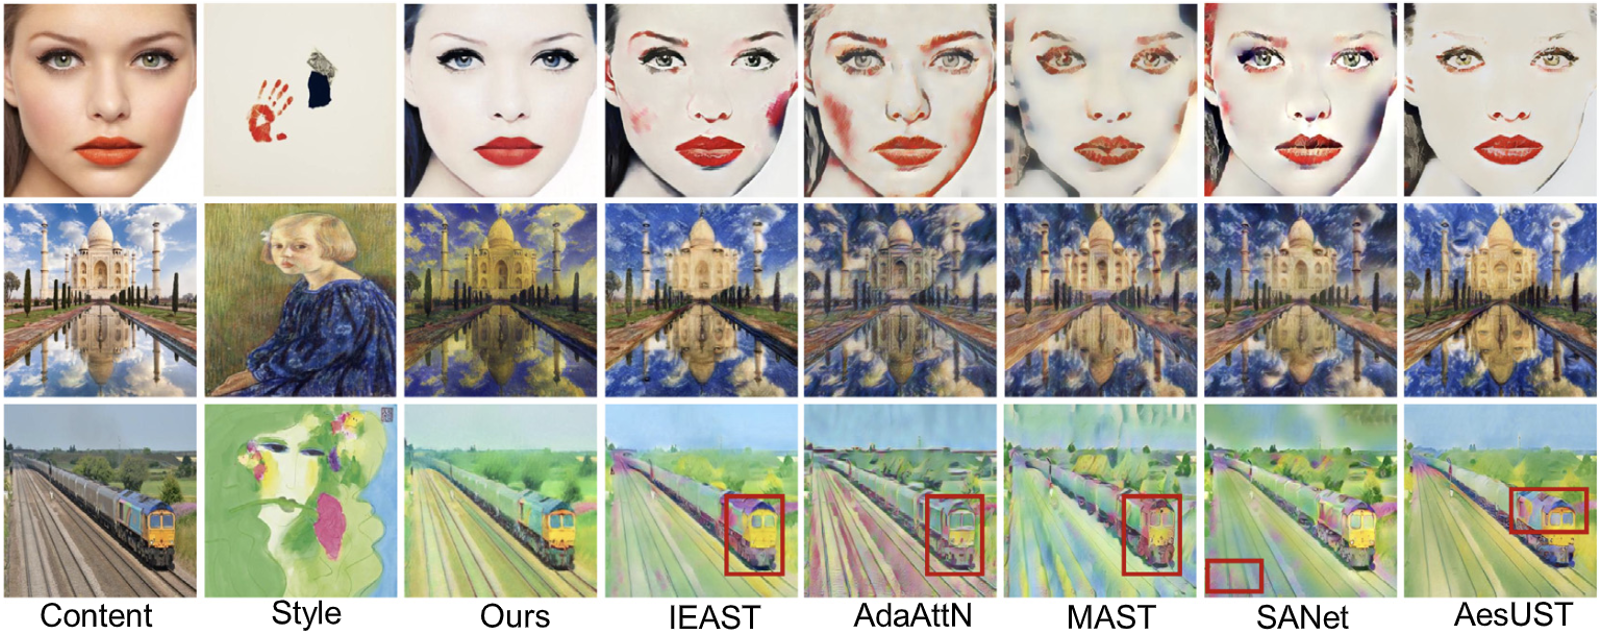
\includegraphics[width=\linewidth]{pics/pic_compare_3.1.png}
    \caption{\label{fig:pic_compare_3_1}风格化结果对比图1}
\end{figure}
\begin{figure}[htbp]
    \centering
    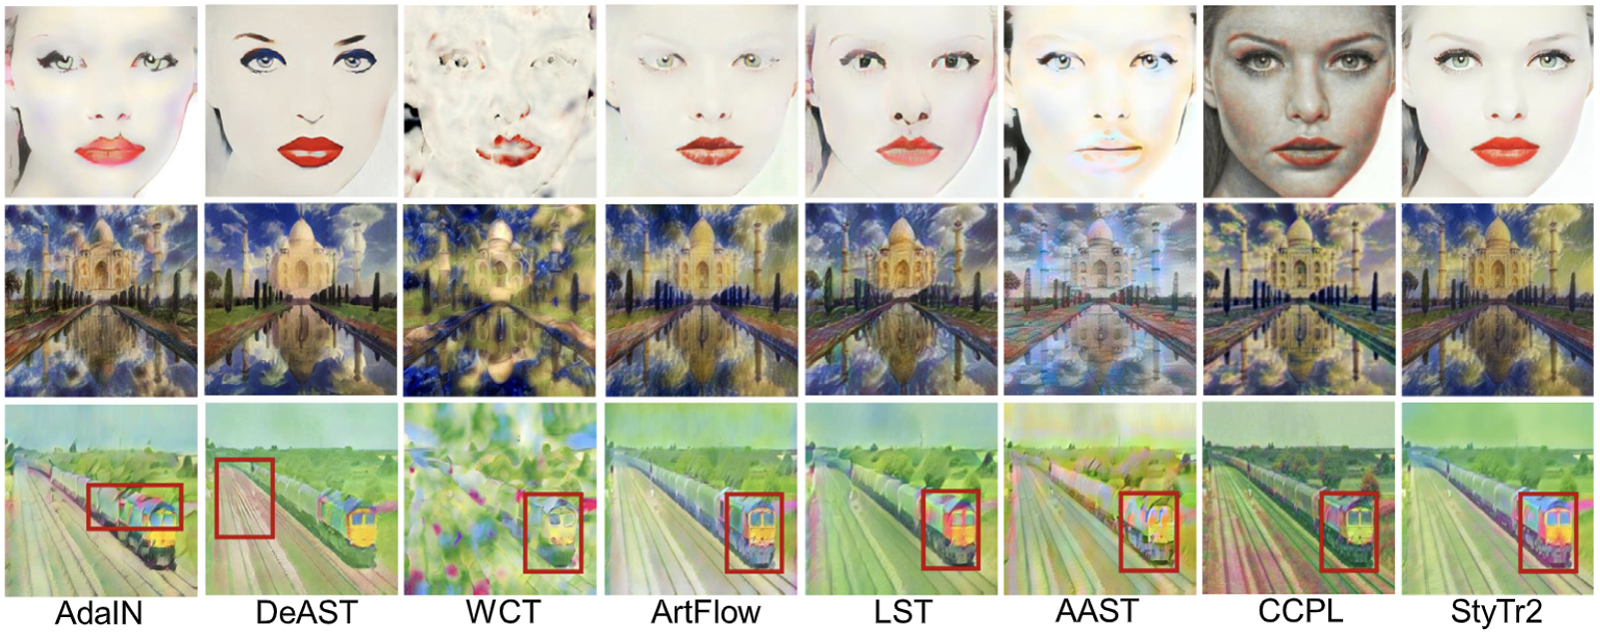
\includegraphics[width=\linewidth]{pics/pic_compare_3.2.png}
    \caption{\label{fig:pic_compare_3_2}风格化结果对比图2}
\end{figure}
\paragraph{定量试验对比和分析}
使用CF、GE、LP、DS四个指标对本章方法产生的结果和其他Sota方法进行风格化质量的定量分析。具体来说,CF 用于衡量内容特征的保存程度,
GE 评估全局颜色和纹理的风格化。LP 根据局部风格的相似性来评估风格化质量。较高的分数意味着更好的风格迁移结果。
DS用于衡量人类用户对于各方法生成的风格化结果的判断。在计算CF、GE、LP的时候,使用 5 个内容和 10 个样式图像对所有的方法进行评估。在计算DS的时候,如前所述,随机选择了 20 张风格化图像,每张图像由 50 个受试者来评价。
定量比较的结果如\autoref{tab:tab_res_compare_3}所示。其中,“推理时间”表示指使用如\autoref{tab:tab_hardware}所示的设备硬件、以端到端方式把512$\times$512像素的图片输入进行推理所消耗的时间。
\begin{table}[htb]
    \centering
    \caption{二维图像风格迁移的定量分析结果}
    \label{tab:tab_res_compare_3}
    \begin{tabularx}{\textwidth}{c X<{\centering} X<{\centering} X<{\centering} X<{\centering}}
        \hline
        & CF $\Uparrow$ & GE+LP $\Uparrow$ & 推理时间 & DS $\Uparrow$ \\ \hline
        WikiArt & - & - & - & 0.784 \\ 
        Ours & \textbf{0.432} & \textbf{1.615} & 1.814 & \textbf{0.573} \\
        IEAST & 0.412 & 1.405 & 0.759 & 0.476 \\ 
        AdaAttN & 0.380 & 1.430 & 1.684 & 0.372 \\ 
        MAST & 0.360 & 1.511 & 1.471 & 0.324 \\ 
        SANet & 0.366 & 1.552 & 0.759 & 0.346 \\ 
        AdaIN & 0.383 & 1.552 & 0.534 & 0.346 \\ 
        CAST & 0.335 & 1.581 & 0.534 & 0.423 \\ 
        WCT & 0.346 & 1.540 & 4.839 & 0.172 \\ 
        LST & 0.408 & 1.459 & \textbf{0.427} & 0.408 \\ 
        StyTr2 & 0.336 & 1.602 & 32.921 & 0.545 \\
        AesUST & 0.420 & 1.524 & 0.783 & 0.568 \\ 
        ArtFlow & 0.411 & 1.505 & 4.530 & 0.356 \\
        AAST & 0.368 & 1.461 & 13.674 & 0.307 \\ 
        CCPL & 0.422 & 1.594 & 0.510 & 0.427 \\ \hline
    \end{tabularx}
\end{table}
可以看出,本章提出的方法在内容保存和感知风格方面的两项客观评价指标以及主观指标中都有较好的表现。同时可以看到该方法也有着较快的速度,可以作为任意风格迁移算法使用。
\subsection{消融实验和分析}
为了确保所提出方法的有效性,在本节中进行了消融分析,其结果如\autoref{fig:pic_abla_3_1},\autoref{fig:pic_abla_3_2}中画红框所示。为了清晰可见,故而采用较大的图排布方式。
可以看到,当去除ICL模块时,风格化图像的质量在内容结构、纹理和笔画笔触的一致性方面会下降。
当去除$L_{Adv}$时,生成的风格化图像表现出明显不和谐的图样和明显的伪影,导致质量下降。这表明对抗性训练对于生成更和谐和逼真的风格化图像是重要的。

\begin{figure}[htb]
    \centering
    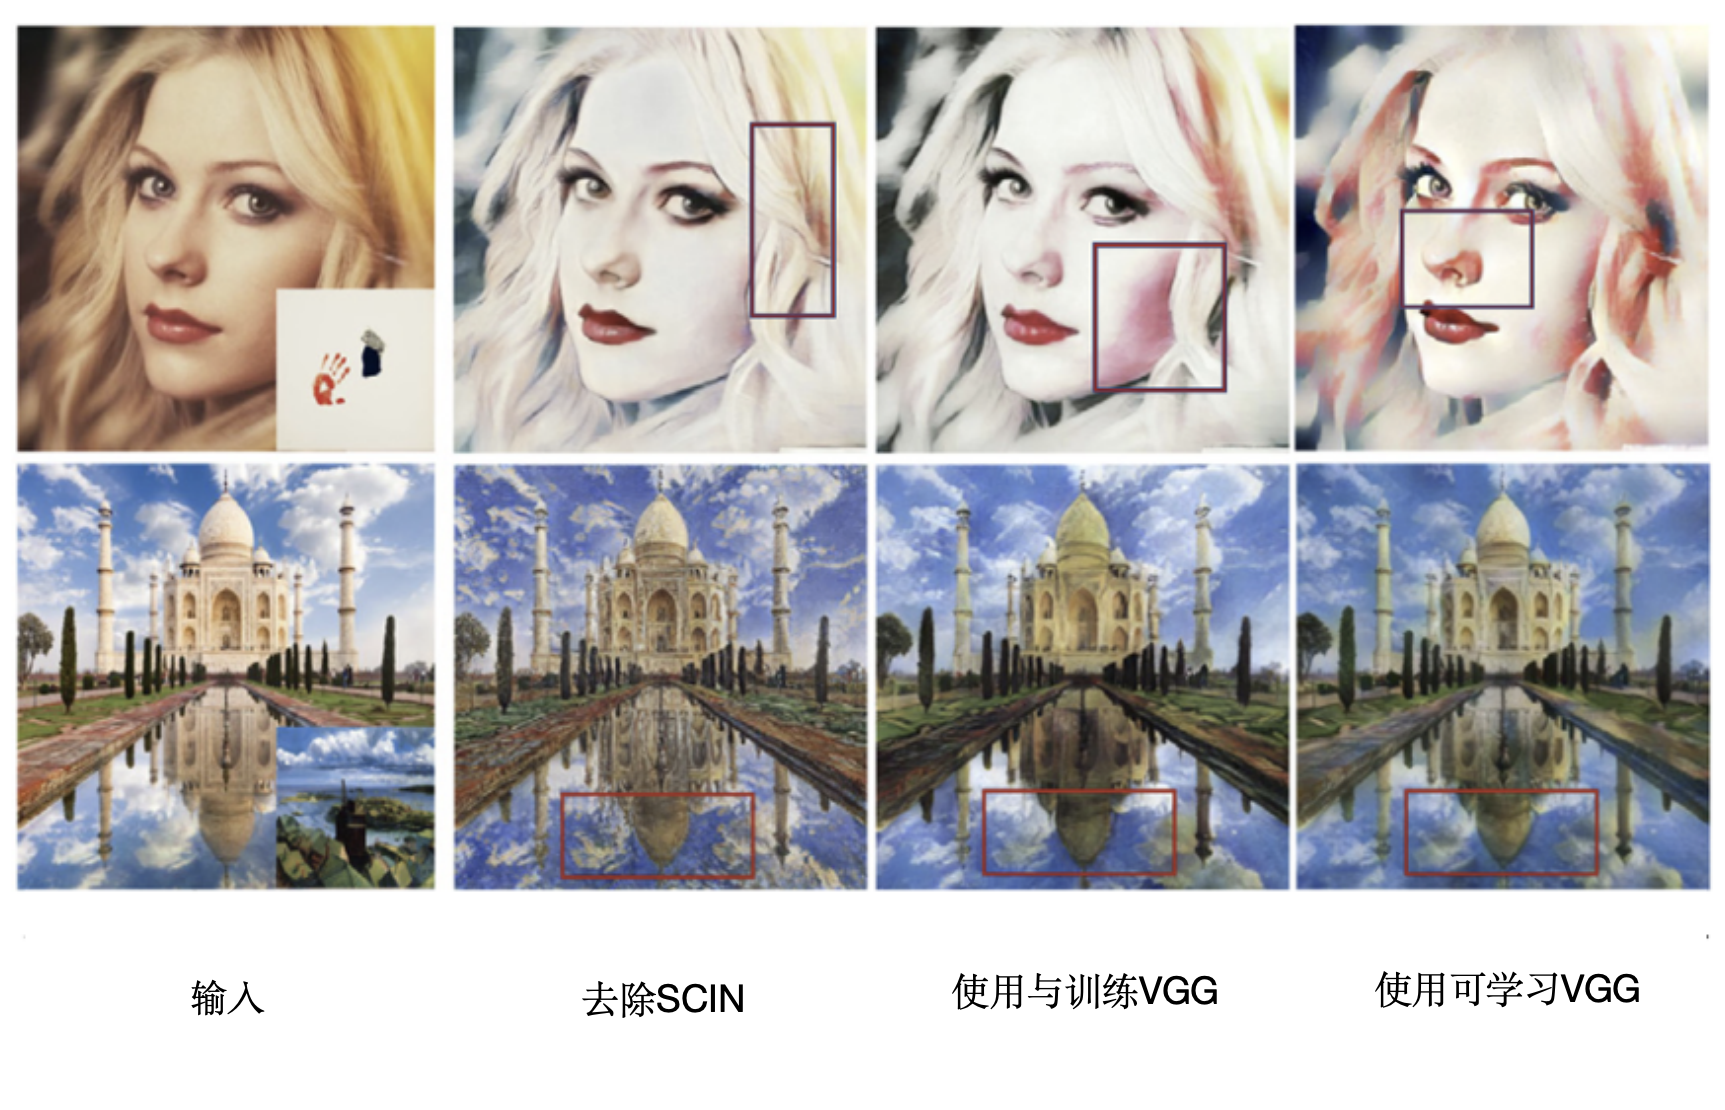
\includegraphics[width=\linewidth]{pics/pic_abla_3.1x.png}
    \caption{\label{fig:pic_abla_3_1}消融实验展示1}
\end{figure}
\begin{figure}[htb]
    \centering
    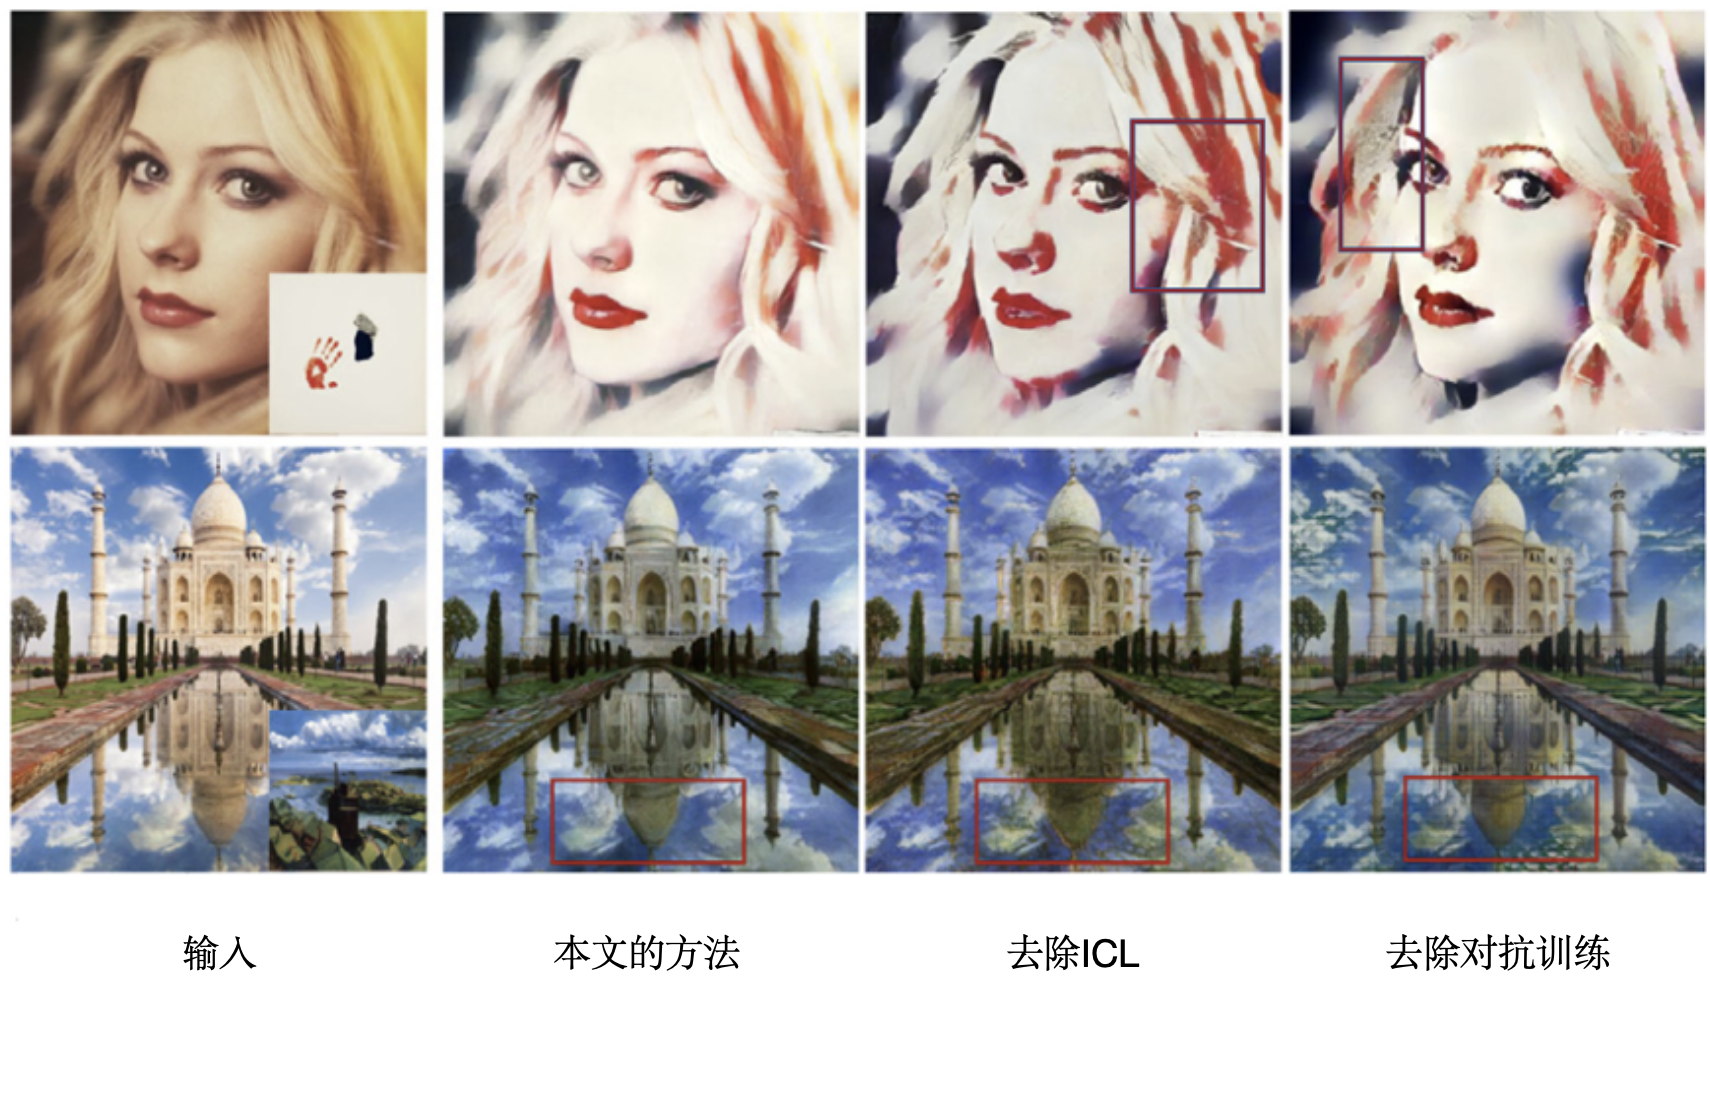
\includegraphics[width=\linewidth]{pics/pic_abla_3.2x.png}
    \caption{\label{fig:pic_abla_3_2}消融实验展示2}
\end{figure}
消融实验还表明,SCIN模块在增强风格化图像和风格图像之间的全局风格一致性方面起着重要的作用。
如果没有 SCIN 模块,可以看到,\autoref{fig:pic_abla_3_2}中的红框区域有波纹形状的笔触,而这是原本所用的风格图中没有的。
风格化结果同风格图像显示出局部的风格不一致。另外,为了证明在ICL模块中,
使用CLIP编码器的效果比VGG好,本节也进行了消融实验。可以看出来使用VGG用于ICL模块中,会导致出现一些伪影。(比如图中红框中左侧的云倒影有不和谐的图样)。
\par 同时本节也对这些消融操作做了定量分析,如\autoref{tab:tab_abla_3}所示。(最高和次高分别用红色、黄色标注)
可以看到本章所述的完整模型的风格特征远好于消融模型,而内容保持特征仅低于可学习的VGG消融,优于其他消融模型。

\begin{table}[htb]
    \caption{\label{tab:tab_abla_3}消融实验的定量分析}
    \begin{tabularx}{\linewidth}{X<{\centering}|X<{\centering}|X<{\centering}|X<{\centering}|X<{\centering}|X<{\centering}|X<{\centering}}
        \hline
        输入   & 全模型 & 去除 ICL & 去除对抗训练 & 去除 SCIN & 使用预训练 VGG & 使用可学习 VGG \\ \hline

        CF    & \textcolor{orange}{0.432}  & 0.423 & 0.414 & 0.431 & 0.426 & \textcolor{red}{0.435}  \\
        GE+LP & \textcolor{red}{1.595} & 1.515 & \textcolor{orange}{1.565} & 1.430 & 1.452 & 1.305 \\ \hline

    \end{tabularx}
\end{table}
\par 同时,为了说明本章提出的感知编码器(PE)的效果,本节中也针对PE模块做了消融实验。现有的基于注意力的方法通常使用SANet作为骨干,
可以学习详细的风格纹理。然而,注意力图是使用VGG的特征向量进行计算的
% (即 $ReLU4\_1$和 $ReLU5\_1$)。
VGG可以有效地捕捉显著的分类特征(如眼睛)。这使得它保留了风格化图像的内容结构,造成了风格化伪影。
为了证明这一点,使用SANet 作为基线模型,分别使用本章提出的感知编码器和固定的 VGG编码器作为变量,渲染出风格化图和注意力图作为比较,如\autoref{fig:pic_abla_pe}所示。

\begin{figure}[htb]
    \centering
    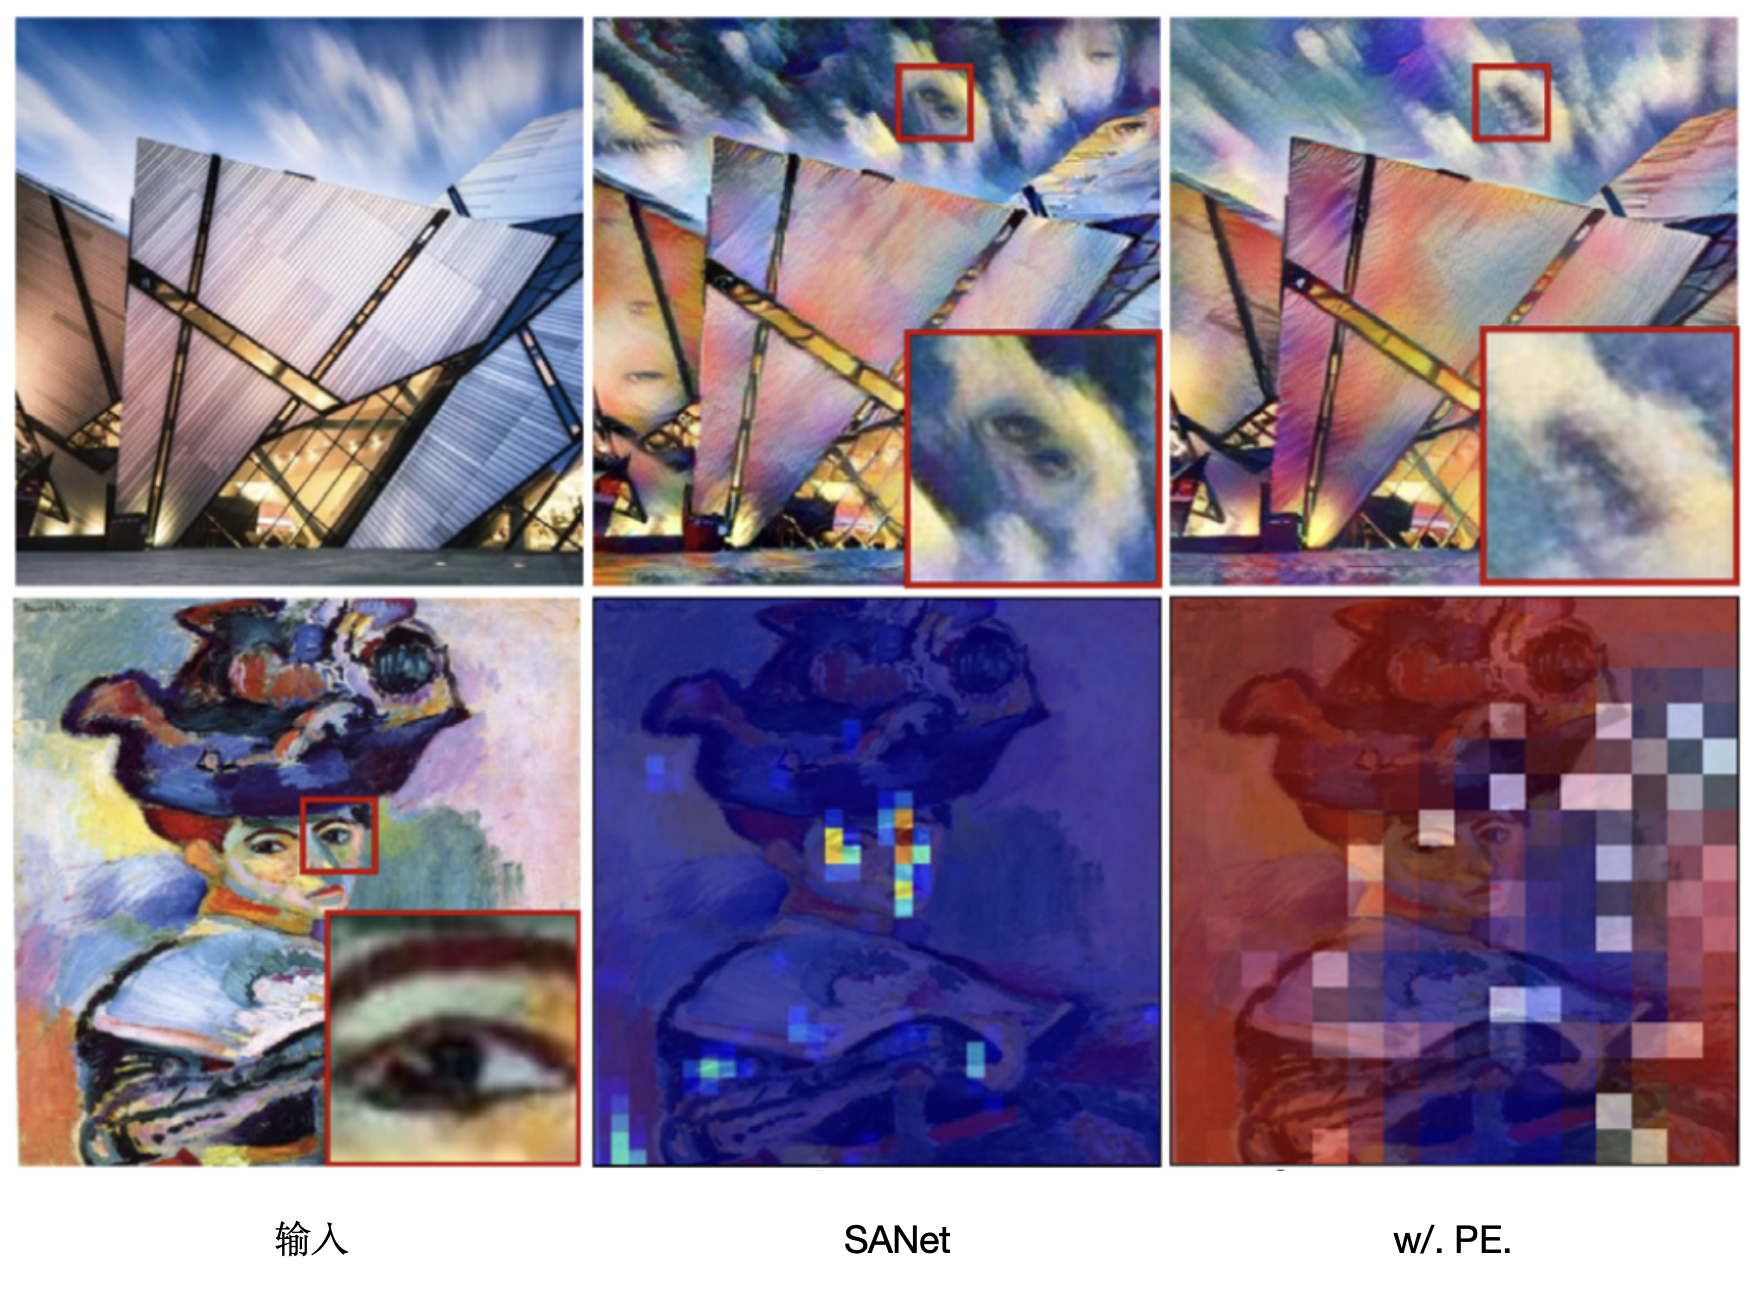
\includegraphics[width=\linewidth]{pics/pic_abla_pe_showx.png}
    \caption{\label{fig:pic_abla_pe}对PE模块的消融实验结果图}
\end{figure}可以看到,在上方的风格化结果中,使用VGG编码的结果图含有人眼这一元素,而使用PE编码器得到的风格化图没有这一元素。并且也可以看到,经由VGG得到的注意力图集中在人脸部区域,而经由PE编码器得到的注意力图较为分散。因此可以认为,本章所提出的PE编码器能够有效捕获风格信息,并且避免过多关注风格图像中如人眼这类的显著分类特征。
\section{本章小结}
本章节提出了一种新颖的网络架构,可以生成高质量的风格化图像。具体来说,本章引入了一种新的风格-内容实例归一化(SCIN)方法,将内容特征与特征空间中的风格特征对齐,实验证明该模块可以更好地生成视觉协调的纹理结果。然后,本章还提出了一种基于实例的对比学习(ICL)方法来学习风格化到风格化的关系,以提高风格化的质量和减少伪影的产生。此外,在本章中分析了使用固定 VGG 作为风格迁移任务中特征提取器的局限性,并提出了一个感知编码器 (PE) 来更有效地捕获样式信息,提升风格化图像的质量。本章第一小节是引言,介绍和对比了前人的研究缺陷,引入本章的研究内容并归纳了本章的研究成果。第二小节是本章的方法介绍,介绍了方法的总述,并逐模块对所提出的方法进行详细说明。第三小节是实验的设计和参数设定,在文中对采用的实验环境配置、实验设定、实验用数据集、实验的评价指标进行了说明。第四小节则对本章提出的方法进行了直观的结果展示,并且也对于许多现有方法进行了对比试验,从定性和定量两个角度对实验结果进行了比对,证明了所提出的方法性能优越。同时也对提出的模块分别进行了消融实验,验证了所述方法的有效性。


\chapter{基于多分辨率哈希网格和可变3D高斯点的零样本三维场景风格迁移方法}
\section{引言}
近年来,随着对3D场景表示方法的研究逐渐深入,人们对3D场景风格迁移的研究兴趣也逐渐增加。
这一任务是3D编辑任务的一个方向,是为了把给定媒介(一般是图像)的风格转移到一个适当表示的三维场景中,
并且不破坏原有场景的内容特征。这一任务的实现通常需要高性能的场景的表示方法作为前提。
现行的方法通常采用点云体素、NeRF~\cite{mildenhall2021nerf}或者3DGS~\cite{kerbl20233d}作为场景表示方法进行建模。使用点云的做法~\cite{huang2021learning,mu20223d,yin20213dstylenet}出现的较早,
由于无法实现零样本的风格迁移并且其本身的场景表达能力有限,其场景的渲染速度和渲染质量都不如新的方法,已经逐渐在这一领域被NeRF和3DGS给替代。
NeRF自其出现开始,就一直被作为一种通用的 3D 场景表示方法,它可以被用于许多任务,比如场景生成和编辑,动态场景渲染,大规模场景渲染等。
NeRF方法有着高保真渲染的能力,并且它的隐式特性能够提供显著的可扩展性,这标志着其比传统的空间表示方法有了更广阔的应用。
这种双重优势使得NeRF表示在3D场景的风格迁移任务中备受关注,并在相当长的一段时间内将其确立为一种基本的场景表示手段~\cite{zhang2022arf,chiang2022stylizing,li2023instant,chen2024upst,liu2023stylerf}。
然而,NeRF依赖高维度多层感知机(MLP)网络对场景数据进行编码,这限制了对特定场景部分的直接修改,并使绘制和场景构图等任务复杂化。
这种复杂性延伸到训练和呈现过程,也导致了渲染和训练的速度过慢,阻碍了实际的应用。
一些改进方法试图解决这个问题,例如 Plenoxels~\cite{fridovich2022plenoxels}、TensorRF~\cite{chen2022tensorf}、和Instant-NGP~\cite{muller2022instant}等。
典型的NeRF把位置和方向嵌入到高维空间来完成训练任务,而Instant-NGP 使用多分辨率散列编码进行位置嵌入,以更快速地完成高质量训练,是最先进的NeRF加速策略之一。
可训练的编码参数共有L个不同分辨率级别,它将特征向量存储在网格的八个顶点上。位置输入通过对其超立方体内的八个顶点的相对位置进行差值,
并对这一结果进行编码。神经网络使用编码特征和方向嵌入结果来合成新的图像。3DGS的出现也从另一个思路进行了加速,它引入了一种强大的场景表示方法,
也通过高度定制化的CUDA实现保障了场景的快速训练和渲染,同时保留了相当高质量的场景细节。
\par 为了成功完成3D场景风格迁移这项任务,采用的风格迁移方法应该确保视图之间的多视图一致性以提供平滑的视觉体验。
尽管2.1小节中所述的2D风格迁移方法在本领域提供了高质量的结果,但直接采用相同的算法用于多视角内容图无法在3D场景视图中提供高度一致的风格化结果。
因此,它们被认为不适合直接用于3D 风格迁移。现有的3D风格迁移方法普遍可以用这样一个流程范式来大致描述:
首先采用特定的能够支持多视图表示的方法对场景本身进行建模表达,然后使用不同的方法把风格图像的风格融合到场景表示中,
再采用解码器组件把新的风格解码出来。现有的几个方法~\cite{saroha2024gaussian,jain2024stylesplat,zhang2024stylizedgs,chen2024gaussianeditor,liu2024stylegaussian}
考虑使用3DGS作为场景表示方法并且进行了场景风格迁移的探索,然而这些方法不会改变表示场景的高斯的位置和形状,这导致场景的某些区域的分辨率较低。
除了上述问题外,现有的3D 风格迁移方法只关注从风格图像中迁移高频模式,比如笔触或颜色统计,而忽略了风格的低频部分,这导致风格化结果不够优良。
同时,部分方法无法做到零样本迁移,或者对算力和硬件要求较高,也存在训练推理速度较慢等问题。
\par 为了解决这些问题,实现一个\textbf{高质量、零样本、低开销的3D任意风格迁移算法},受到Instant-NGP~\cite{muller2022instant}这一工作的启发,
本章提出使用多分辨率哈希网格(Multi Resolution Hash Grid,MRHG),通过对每个高斯点的颜色增量进行查询,实现零样本迁移和存储风格信息。
对于每个高斯点,将其位置信息输入到MRHG中查询得到包含了位置信息的风格特征向量,
再把该风格特征向量和风格图经过编码器产生得到的风格向量和一起输入到小型MLP中,获得对应于某特定风格下的每一个高斯点的颜色属性增量,
最后将其加起来得到新的高斯点颜色属性。为了更好地模拟风格这一概念,本章认为可以适当地对场景高斯进行一些调整,
以更好地匹配风格图的笔触等抽象信息。为此本文对于高斯点的其他属性采用分层更新的策略,并且仅对较外层的高斯点的位置和旋转属性进行小幅度微调,
这一操作减少了所需的计算量并且也能有效提高风格化质量。把更新过后的高斯点输入到原本的3DGS投影和渲染管线中即可得到风格化后的结果。
\par 在本章中,专注于高质量场景的零样本风格化任务,并且做了充分的理论说明和实验验证。本章的主要贡献如下:
\begin{itemize}
    \item 提出了一种新的场景风格迁移方法,它具有快速渲染的特性,并且能够支持零样本的场景任意风格迁移和较高的风格化质量。
    \item 提出使用多分辨率哈希网格来存储每个风格的全局和局部信息,以较少的计算量和参数量实现了风格信息嵌入到高斯点内,实现零样本风格化推理;并且采用分层的方法对部分高斯点进行针对性控制,以更好地学习到风格图中除了颜色以外的其他艺术信息,提升风格化的效果。
    \item 进行了大量的实验,从定性和定量两个方面证明了本章所提方法是有效的和性能优越的,它能够做到在商用GPU上进行快速渲染和训练,能以零样本的方式高质量地把风格从风格载体迁移到场景中。
\end{itemize}

\section{方法介绍}
\subsection{总述}
该方法的概述如下:首先使用3DGS~\cite{kerbl20233d}的代码和训练流程,使用colmap~\cite{schoenberger2016sfm}对图片集进行处理得到SfM点,用之进行初始化并且使用第零阶段损失\(L_{Stage0}\)端到端地训练好一个场景的高斯表达。
在训练的时候就根据其致密化轮次对场景中的高斯点进行分层标记,分层可以实现对于部分高斯点的精确控制,具体的分层方式和分层约束如第4.2.3小节所述。
在获得了一个训练好的场景表达后,结合如\autoref{fig:pic_main4}所示的网络架构图,该风格化网络训练方式如下:首先冻结3DGS管线中全部组件,
使用一阶段损失\(L_{Stage1}\)和训练好的高斯点集对MRHG、增量MLP和全连接层进行训练,学习风格的低级特征如颜色等的迁移。
训练完成后,冻结上述组件,使用二阶段损失\(L_{Stage2}\)对TinyMLP进行训练,在现有的模型基础上继续优化,通过改变高斯点的位置和协方差属性更好地学习风格的笔触、线条等特征。

\begin{figure}[htb]
    \centering
    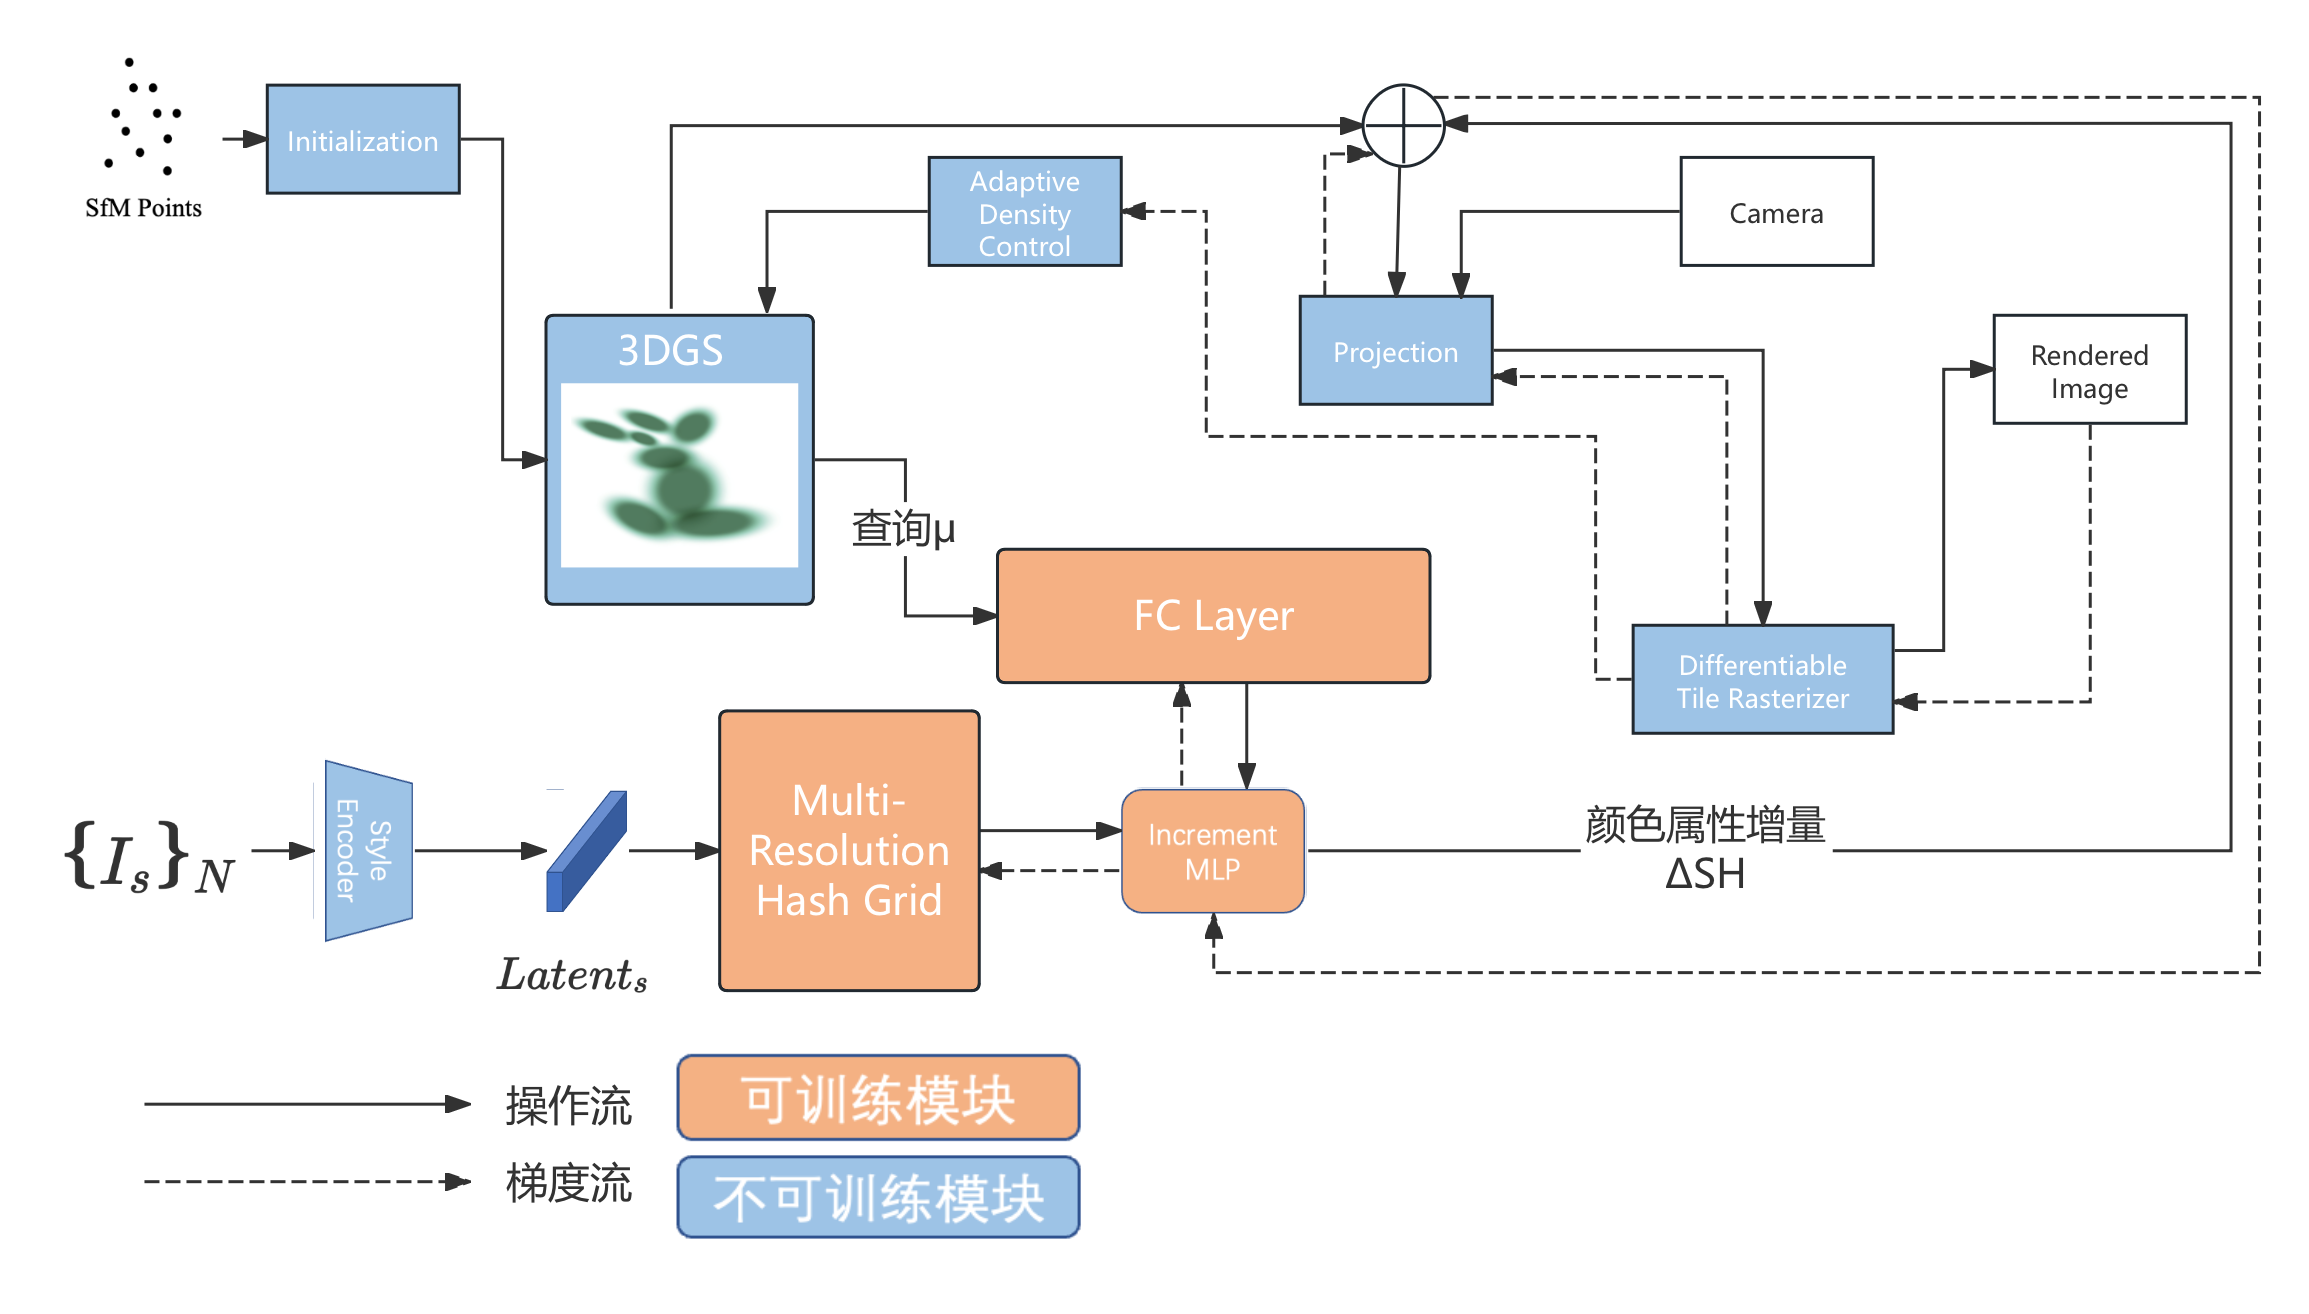
\includegraphics[width=\linewidth]{pics/mainpic4.png}
    \caption{\label{fig:pic_main4}本章所述模型的主结构图}
\end{figure}
\subsection{多分辨率哈希网格设计}
由于需要对大量的点进行查询,使用全连接神经网络编码的神经图形原语在训练和评估过程中花费是非常昂贵的。多分辨率哈希编码~\cite{muller2022instant}的设计则天然地降低了计算的开销。
该设计采用了一个灵活的编码器,这使得可以使用一个较小的神经网络来降低浮点数和访问内存的开销同时几乎没有质量的损失。这个较小的神经网络利用多分辨率哈希网格中的可学习特征向量来增强,
同时多分辨率的结构天然地可以避免哈希冲突。另外原作者对其进行了充分的优化,采用CUDA实现它的计算,能够有效减少带宽和计算开销。
这一操作的本质特征是将一组网格与特征向量数组进行映射,以让特征向量数组存储更多的信息。在一个较粗的分辨率下是一一对应;
在精细分辨率下将特征向量数组处理为哈希表格,使用空间哈希函数使网格与其进行映射。因为空间哈希冲突会使冲突的区域梯度趋于平均,
于是梯度较大的区域会占支配地位。也就是说这样的设计使得哈希冲突反而让那些精细的稀疏区域能够自动地得到更优先的处理,
同时兼顾粗分辨率部分,得到更好的细节。这一查询的时间复杂度仅为\(O(1)\)。
本文采用的多分辨率哈希网络设计如下:采用L级分辨率的网格来存储每个点的附加信息,
每一个$l$都对应于一个分辨率\(N_l\),其含义是把整个空间划分为\(N_l\times N_l\times N_l\)个小立方体,\(N_l\)可以如\autoref{equ:cal_mrhg_res}计算。
%短公式

\begin{equation}
    \label{equ:cal_mrhg_res}
    \begin{aligned}&N_l{:}=\lfloor N_{min}\cdot b^l\rfloor,\\&b{:}=\exp{(\frac{\ln N_{max}-\ln N_{min}}{L-1})}\end{aligned}
\end{equation}
其中,\(N_{max}\)和\(N_{min}\)是拟定的最大和最小分辨率,$b$是每一级分辨率间的公比。
\par 对于每一个输入的三维坐标$(x,y,z)$,查询其在每个第l级分辨率的网格下对应的八个角点的坐标,
并且用异或运算哈希映射把这个八个坐标映射到八个哈希索引$h(\mu)$,其计算如\autoref{equ:cal_mrhg_hash}所示。其中d可取1,2,3,分别代表xyz三个位置维度。
$\pi$是一组大素数集合,在本文中取\(\pi_{1}:=1,\pi_2=2654435761,\pi_3=805459861\),$T$是哈希表的表长,$\bigoplus $为异或操作。
\begin{equation}
    \label{equ:cal_mrhg_hash}
    h(\mu)=\left(\bigoplus_{i=1}^d\mu_i\pi_i\right)\mathrm{mod}T
\end{equation}
\par 用线性插值方法根据八个索引检索哈希表得到该点在第$l$级分辨率的
向量特征\(\mathrm{f}(h(\mu);l)
\in\mathbb{R}^F\),
并且把它们拼接在一起构成一个点的位置编码信息\(f(\mu)\),
如\autoref{equ:cal_mrhg_f}所示。
\begin{equation}
    \label{equ:cal_mrhg_f}
    f(\mu)=cat([f(h(\mu);0),f(h(\mu);1),\ldots,f(h(\mu);L-1)])\in\mathbb{R}^{L*F}
\end{equation}


本章中的MRHG原理示意图如\autoref{fig:pic_mrhg}所示:

\begin{figure}[htb]
    \centering
    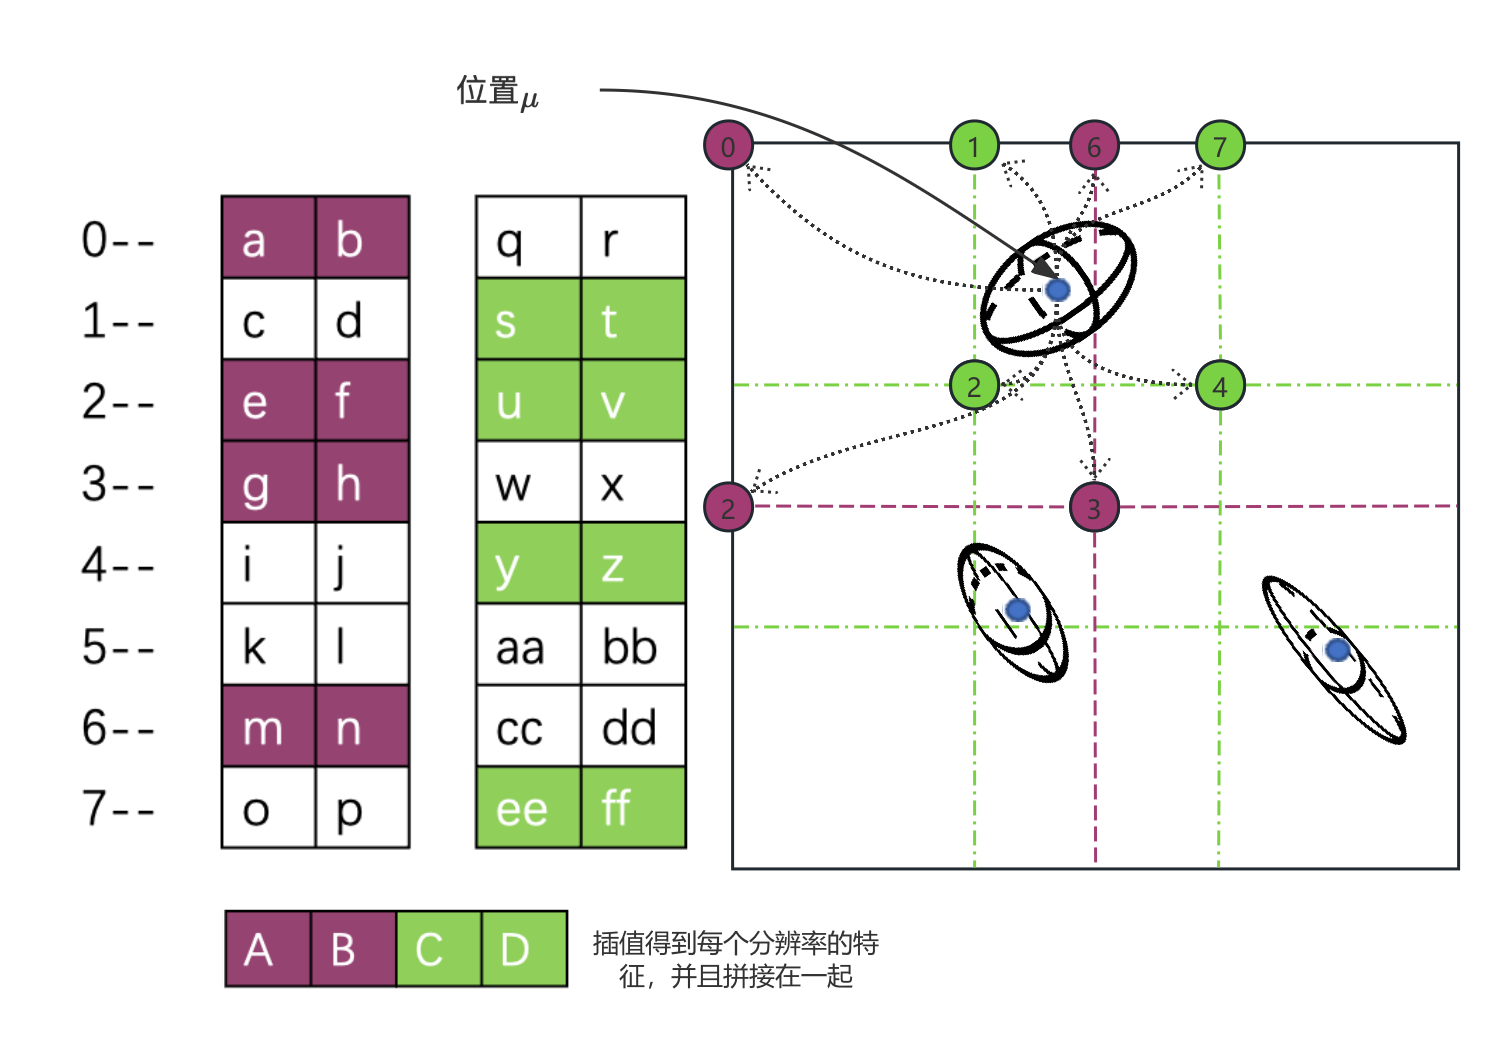
\includegraphics[width=\linewidth]{pics/pic_mshg.png}
    \caption{\label{fig:pic_mrhg}MRHG原理示意图}
\end{figure}




随后,使用MLP进行维度匹配,将MRHG输出的查询结果结合风格图编码向量信息一起用MLP映射到对应的48维向量,用以表征模型中的SH属性的增量。

\subsection{层次化高斯点的分布和锚函数的设计}
由于现有的用3DGS表示场景进行风格迁移的方法不会改变高斯的位置和形状,这导致风格化的场景的某些区域的分辨率较低,
同时,考虑到场景的风格化不是简单的改变场景的颜色,而是需要学习一些笔触等更加复杂的信息,想要做到这些就要求在风格化的时候改变场景的形状。
如\autoref{fig:pic_diff_4}所示,左侧分别是内容场景和风格图,中间和右边分别是两种方式进行的风格化,可以看出来右边的方式是更好地学到了笔触等复杂风格信息,
而中间的方法只有颜色变换。但是,考虑到全部的高斯点数量巨大,完全更改全部的高斯点的位置和协方差属性会导致效率低下和计算资源占用,
是次优的方案。本章认为可以仅对外层的一部分点进行位置的微调以满足上述需求,这也和人们的直觉是相符的。
\begin{figure}[htb]
    \centering
    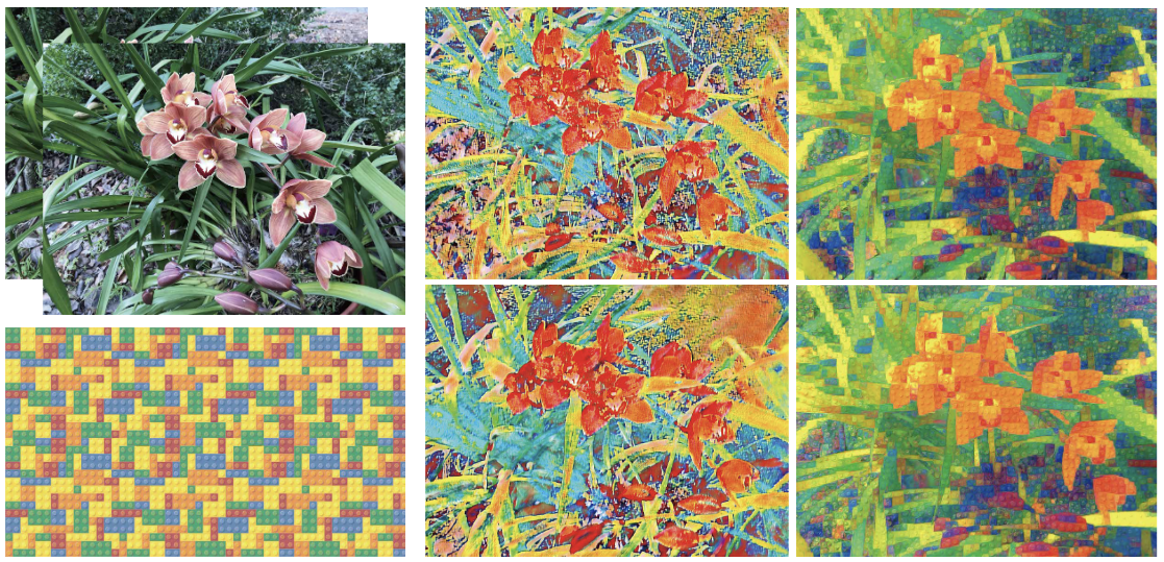
\includegraphics[width=\linewidth]{pics/pic_4_diff.png}
    \caption{\label{fig:pic_diff_4}两种风格化方式的差异}
\end{figure}
从GaussianEditor~\cite{chen2024gaussianeditor}得到的灵感,本章采用分层高斯飞溅 (HGS)进行这一操作,这是一种更适合生成和编辑场景的GS的结构化表示。
和GaussianEditor中不同的是,本文中偏移由风格图像的风格特征$Latent_s$控制,因此考虑使用MLP来进行这一优化。
提出的小型MLP接受$Latent_s$作为输入,并且输出高斯点的位置和协方差属性值。
为了防止输出的属性值同原来的属性值差异过大造成失真,引入锚点损失进行约束。
HGS根据产生特定高斯点的致密化轮次将GS分类为不同的代。
初始高斯$\Theta$的轮次为0,在训练过程中,第k个致密化轮中生成的点的轮次被标记为k。
随后,对来自不同轮次的高斯点施加不同的约束来控制它们的灵活性程度。
约束方式为仅对轮次值大于某个阈值$\theta$的高斯点启动优化,并使用锚点损失用于强制执行这一约束。
在训练开始时,HGS将所有符合轮次阈值的高斯函数的属性记录为锚点。
后和3DGS原本的设定不同,在本章中使用神经网络对这些锚点的颜色和协方差属性进行直接更新。
在训练期间,使用锚点状态和当前状态之间的MSE损失(如\autoref{equ:cal_anchor_p}所示)来确保高斯属性不会偏离它们各自的锚点过多。
经过训练的神经网络可以在小幅度范围内对少量的高斯点的位置和协方差属性进行更新,以更好地满足风格的高阶特征迁移。
\begin{equation}
    \label{equ:cal_anchor_p}
    \mathcal{L}_{anchor}^P=\sum_{\mathbf{n}}\lambda_{pi}(P_i-\widehat{P}_i)^2
\end{equation}
其中n表示高斯的总数,P表示当前高斯的某个属性,包括位置、协方差属性,其值可以取x、s、q。
这里,$\widehat{P}$指的是锚状态中记录的相同属性。术语$\lambda_{pi}$表示应用于第$i$个高斯点的锚点损失的强度,
该损失根据其轮次值变化而变化。本步骤中的训练损失定如\autoref{equ:cal_anchor_L}所示。

\begin{equation}
    \label{equ:cal_anchor_L}
    L_{anchor}=\sum_{P\in\{x,s,q\}}\lambda_PL_{anchor}^P
\end{equation}
HGS 中的这种生成设计防止了MLP生成的GS属性值过度灵活的问题。对于较早致密化生成的高斯点不做修改,只对后生成的高斯点进行位置和协方差的微调,因此,它能够让场景的几何根据风格的一些高阶特征进行微调。这种方法确保了随机损失下保持场景几何形成大致不变,以更好地执行风格化任务。
\subsection{损失函数}
本章采用多种损失函数来约束网络的训练,具体包括:感知内容损失$L_C$、感知风格损失$L_S$、锚损失$L_{anchor}$、最近邻特征匹配损失$L_{NNFM}$、
差分结构相似性指数损失$L_{D-SSIM}$。其中损失$L_C$、$L_S$已经在上一章进行了介绍,损失$L_{NNFM}$在第2.2节进行了介绍,
损失$L_{anchor}$在上一小节进行了介绍。下面将具体地对$L_{D-SSIM}$这个损失和本章中采用的三个阶段损失进行介绍。
\paragraph{差分结构相似性指数损失}
在第2.4节中已经详细介绍了SSIM的概念和计算方法。这是一个用于约束图像结构相似的指标,在风格迁移或其他图像处理任务中,
D-SSIM损失可以用来确保生成的图像在结构上与目标图像保持一致。通过最小化D-SSIM损失,可以提高生成图像的视觉质量,
使其在结构上更接近于参考图像。给定原图$I_C$和渲染生成的图像$I_R$,其计算方式如\autoref{equ:cal_dssim_loss}所示。
\begin{equation}
    \label{equ:cal_dssim_loss}
    \mathcal{L}_{D-SSIM}=1-SSIM(I_R,I_C)
\end{equation}
\paragraph{第零阶段损失}
本章使用$L_{Stage0}$来进行3DGS的训练,和原论文的设定一样,首先对模型生成的图片$I_R$和原本的数据集图片$I_C$应用$L_{D-SSIM}$和$L_1$进行约束,
训练得到一个高质量的3D场景的高斯表达。如\autoref{equ:cal_stage0_loss}所示。
\begin{equation}
    \label{equ:cal_stage0_loss}
    \mathcal{L}_{Stage0}=\mathcal{L}_1+\lambda_0\mathcal{L}_{\text{D-SSIM}}
\end{equation}
\paragraph{第一阶段损失}
使用$L_{Stage1}$来进行多分辨率哈希网格和增量网络的训练,以求网络能够学会零样本的颜色迁移知识。
对模型生成的风格化图片同风格图、内容图进行约束,采用的$L_{Stage1}$由两部分组成,如\autoref{equ:cal_stage1_loss}所示。
\begin{equation}
    \label{equ:cal_stage1_loss}
    \mathcal{L}_{Stage1}=\mathcal{L}_C+\lambda_1\mathcal{L}_\mathrm{S}
\end{equation}
\paragraph{第二阶段损失}
使用$L_{Stage2}$对HGS和TinyMLP进行训练,以让模型学会根据风格图中的笔触和线条自适应地改变一部分场景的外形,
获得更高的风格化质量。$L_{Stage2}$由锚损失和NNFM损失构成,前者用于约束外形的变化幅度,后者用于约束模型学习复杂的高频视觉细节,如\autoref{equ:cal_stage2_loss}所示。
\begin{equation}
    \label{equ:cal_stage2_loss}
    \mathcal{L}_{Stage2}=\mathcal{L}_{Anchor}+\lambda_2\mathcal{L}_{NNFM}
\end{equation}
\section{实验设计和参数设定}    
\subsection{实验环境配置}
本算法基于Python语言和Pytorch~\cite{paszke2019pytorch}深度学习框架实现,3DGS部分的代码使用了Kerbl等人的实现~\cite{3dgsrepo},
分辨率哈希编码部分借鉴和参考了github作者yashbhalagt的实现~\cite{ingp-torchrepo}
HGS部分参考了GaussianEditor的官方实现~\cite{gaussianeditorrepo},
实验环境中的硬件配置信息同\autoref{tab:tab_hardware}一样,软件版本信息如\autoref{tab:tab_software_4}所示。
\begin{table}[htbp]
    \caption{\label{tab:tab_software_4}第四章实现的软件配置信息}
    \begin{tabularx}{\linewidth}{c|X<{\centering}}
        \hline
        操作系统 & Linux 6.5.0-35-generic \#35~22.04.1-Ubuntu \\ \hline
        NVIDIA驱动 & 535.171.04 \\ \hline
        CUDA & V11.8.89 \\ \hline
        Python & 3.7.6 \\ \hline
        PyTorch & 1.13.1+cu116 \\ \hline
    \end{tabularx}
\end{table}

\subsection{实验设置}
本章提出的模型分训练阶段和测试阶段。训练阶段分三步,首先完全参照3DGS~\cite{kerbl20233d}
的训练流程和超参数,使用对应的数据集和colmap~\cite{schoenberger2016sfm}生成SfM点集,再使用SfM点进行训练得到一个场景的高斯表达$\{G_0\}$。
然后冻结3DGS管线中全部组件,使用一阶段损失$L_{Stage1}$和训练好的高斯点集$\{G_0\}$对MRHG、增量MLP和全连接层进行训练,
学习风格的低级特征如颜色等的迁移。在训练中采用学习率为0.0001的Adam优化器~\cite{diederik2014adam}进行训练,
批次大小设置为8,训练轮次为50000。训练完成后,冻结上述组件,使用二阶段损失$L_{Stage2}$对TinyMLP进行训练3000轮,
以在现有的模型基础上继续优化,通过小幅度地改变部分高斯点的位置和协方差属性,更好地让场景渲染图匹配风格的笔触、线条等特征。
在训练的时候,设定\(\lambda_0=0.25\text{,}\lambda_1=0.33\text{,}\lambda_2=0.1\);
在多分辨率哈希编码相关的参数中,设定$L$为16,$T$为$2^{12}$,$F$=8,$N_{min}$和$N_{max}$分别为16和512。
本章实验所用的风格图像统一设定长宽为256。\autoref{fig:pic_main4}中的FCLayer是一个单层全连接层,它把输出的风格潜码转变维度到64,
并与多分辨率哈希查询得到的向量拼接到一起输入增量网络。增量网络输出48维的颜色增量。
\par 推理阶段,网络经过充分训练,已经具有了零样本风格迁移的能力。本章所提出的模型使用$\{G_0\}$和全部的3DGS渲染管线进行推理,模型接受风格图像输入,
得到一个风格化的场景表达,并且用它渲染出新视角的风格化图像。
\subsection{实验数据集}
本章训练时所用的风格图全都来自WikiArt数据集~\cite{wikiart2018}。
所用的场景数据集为Mip-NeRF 360数据集~\cite{barron2022mip}和Tanks and Temples数据集~\cite{knapitsch2017tanks}。
\paragraph{Mip-NeRF 360数据集}
Mip-NeRF 360数据集最一开始用于训练和测试Mip-NeRF 360模型。该数据集包含大量的室内和室外场景的静态图像,用于训练模型以合成高质量的3D场景和模型。
数据集的来源主要是通过采集现实世界中的无界场景,包括各种复杂的环境和物体,以确保模型的泛化能力‌。该数据集包含9 个场景(5 个室外和 4 个室内),
每个场景都包含一个复杂的中心对象或区域和详细的背景。数据集的特点为:
\begin{itemize}
    \item 高质量:能够用来生成高度逼真的视图和详细的深度图
    \item 无界场景支持‌:能够在无界场景中生成真实的渲染,减少模糊和低分辨率的问题。
\end{itemize}
\paragraph{Tanks and Temples数据集}
‌Tanks and Temples‌是一个用于3D重建的基准测试数据集,由Intel Labs于2017年在SIGGRAPH上发表。该数据集包含14个场景,
包括单个物体(如坦克和火车)以及大型室内场景(如礼堂和博物馆),旨在用来评估3D重建算法在复杂场景下的性能‌。它由以下部分组成:
\begin{itemize}
    \item‌ 训练数据:包含训练用的数据集。
    \item 测试数据:包含测试用的数据集,进一步分为中级和高级‌两个级别,分别用于评估算法在不同难度下的表现‌。本节中主要使用中级级别中的数据集Caterpillar和truck进行训练和评估。
\end{itemize}
\subsection{评价指标}
本节将从三维场景的长短程一致性和生成图像的风格化质量两个方面对结果进行评估。在场景的一致性方面,遵循先前在本文第2.4节中的描述,
把渲染得到的不同视图当作一个视频对待,使用\(\mathcal{E}_\text{consistency}(\tilde{\mathcal{J}}_u,\tilde{\mathcal{J}}_v)\)
对渲染结果的一致性进行分析作为模型的一致性指标。
\par 同时,在评估风格化图像的质量方面,本节亦使用本文第2.4节叙述的ArtFID指标和SSIM指标来衡量图像的结构保存程度和艺术性。
\section{实验结果和分析}
在本节中,首先对于提出的方法在数据集上进行实验后获得的风格迁移结果进行展示,然后展示本算法与近年来表现较好的一些开源的三维场景风格迁移算法之间的效果对比,包括定性对比与定量对比,最后对本算法中提出的创新模块进行消融实验以验证该模块的有效性。
\subsection{实验结果展示}
本小节随机选择了两个风格图和来自两个数据集的各一个场景,分别是bicycle场景和truck场景,每个场景使用五个视角,以全面观察风格化场景的效果。
经过充分实验,得到了一些风格化图像,并将其展示在\autoref{fig:pic_4_show_res}中。可以看到本章所述的方法很好地进行了风格化,并且含有了一部分绘画的风格笔触。
\begin{figure}[htbp]
    \centering
    \includegraphics[width=.8\linewidth]{pics/pic_show4_1.png}
    \caption{\label{fig:pic_4_show_res}场景风格化展示图}
\end{figure}
\subsection{对比试验和分析}
本小节随机选择了八个风格图和来自两个数据集的各两个场景,每个场景选择两个视角进行了实验并且得到了一些风格化图像,同时也针对这些图像结果进行了定量分析和评估,对比试验的结果放在下文。
\paragraph{定性实验对比和分析}
如\autoref{fig:pic_4_cmp_res1}和\autoref{fig:pic_4_cmp_res2}所示,随机选取了八个风格图,并将所提出的方法与最先进的方法在两个数据集的各两个场景上进行比较,本章所述方法的对比对象包括StyleGaussian~\cite{liu2024stylegaussian},
StyleRF~\cite{liu2023stylerf},G-style~\cite{kovacs2024g}, 同时为了验证说明本方法的风格化质量较高,在本节中也和AdaIN~\cite{huang2017arbitrary}做了对比,以更好地评估本方法风格化视觉效果。
图中最左边一栏依次给的是场景图和风格图。可以看到本章所述的风格化方法拥有不输于经典的2D风格化方法的颜色均衡性和协调性,
也没有出现局部的颜色不均匀和伪影等。G-style方法保留了背景图的颜色和显著的内容细节,
StyleRF在采用的MipNerf 360数据集~\cite{barron2022mip}上表现不佳,StyleGaussian方法在部分场景和风格条件下的结果难以辨认。
\begin{figure}[htb]
    \centering
    \includegraphics[width=\linewidth]{pics/pic_compare4_1.png}
    \caption{\label{fig:pic_4_cmp_res1}对比结果图1}
\end{figure}
\begin{figure}[htb]
    \centering
    \includegraphics[width=\linewidth]{pics/pic_compare4_2.png}
    \caption{\label{fig:pic_4_cmp_res2}对比结果图2}
\end{figure}
\paragraph{定量试验对比和分析}
在本小节中,使用长程和短程一致性指标,对本方法的结果和其他方法进行场景风格化一致性的定量分析。使用ArtFID和SSIM对风格化的效果进行定量分析。结果如\autoref{tab:tab_res_compare_4}所示,
最高和次高分别用红色、黄色标注。可以看出,本章提出的方法能够做到在风格化效果对标2D风格化方法的同时,保持了场景的较高一致性。
\begin{table}[htb]
    \centering
    \caption{三维场景风格迁移的定量分析结果}
    \label{tab:tab_res_compare_4}
    \begin{tabularx}{\textwidth}{c X<{\centering} X<{\centering} X<{\centering} X<{\centering} X<{\centering}  X<{\centering} }
        \hline
         & Short-range        & Consistency       & Long-range          & Consistency        &  &  \\
         方法   & LPIPS $\Downarrow$ &  RMSE $\Downarrow$ &  LPIPS $\Downarrow$&  RMSE $\Downarrow$ &       ArtFID $\Downarrow$ & SSIM $\Uparrow$  \\ \hline
        Ours & \textcolor{orange}{0.030}        & \textcolor{red}{0.033} & \textcolor{red}{0.069}   & \textcolor{red}{0.071} & \textcolor{orange}{19.7} & \textcolor{orange}{0.53}   \\ 
        StyleGaussian & \textcolor{red}{0.029} & \textcolor{orange}{0.033} & \textcolor{orange}{0.080} & \textcolor{orange}{0.082} &  35.5  & 0.49  \\ 
        StyleRF & 0.051            & 0.040            & 0.130            & 0.098            &    39.7        &  0.42 \\ 
        G-style & 0.060           & 0.036        & 0.101            &  \textcolor{orange}{0.079} &  30.1          &0.51 \\ 
        AdaIN & 0.111   & 0.087         & 0.162             & 0.135          & \textcolor{red}{18.5}        & \textcolor{red}{0.55} \\ \hline
    \end{tabularx}
\end{table}
\subsection{消融试验和分析}
在本节中,进行了消融分析,以评估所提出HGS在学习风格笔触方面的有效性,其结果如\autoref{fig:fig_abla_4}中画红框所示。
其中W/. HGS代表使用完整模型,W/O HGS代表不使用HGS部分。可以看到,对于采用的风格图,使用HGS的设计和有效地强化了风格图的笔触和线条信息,
比如红框中的树和车架部分,有着更加好的视觉效果。

\begin{figure}[htb]
    \centering
    \includegraphics[width=\linewidth]{pics/pic_abla4_1.png}
    \caption{\label{fig:fig_abla_4}对于HGS的消融实验结果图}
\end{figure}

\par 在本小节中也对这一消融操作做了定量分析,比较消融模型和完全模型的ArtFID和SSIM两个分数,如\autoref{tab:tab_abla_4}所示,可以看到完整模型的风格特征好于消融模型,
这充分证明了前述方法中对外围的高斯点执行分层可变形的训练策略是有效果的。
\begin{table}[htb]
    \caption{\label{tab:tab_abla_4}对HGS的消融定量分析结果表}
    \begin{tabularx}{\linewidth}{c  X<{\centering} X<{\centering}}
        \hline
          & W/. HGS & W/O HGS \\ \hline
        ArtFID $\Downarrow$  & 19.7 & 25.2 \\ 
        SSIM $\Uparrow$  & 0.53 &  0.50 \\ \hline
    \end{tabularx}
\end{table}
\section{本章小结}
本章节提出了一种新颖的场景风格迁移方法,它具有快速渲染的特性,可以生成高质量的风格化场景。具体来说,本章把多分辨率哈希网格这一高效、紧凑、自适应的结构应用于3DGS的颜色增量查询,以高效地实现零样本的场景风格化推理。同时,为了更好地拟合风格的笔触和线条等高阶信息,采用了分层高斯和小型MLP结合的手段,对GS模型的位置和协方差信息进行了小幅度的微调,有效地提升了风格化的视觉效果。同时,本章也进行了大量的实验,其中,通过对比实验证明了本方法在风格化质量上是更优的,并且通过消融实验证明本章提出的改进是有效的。
\par 本章第一小节是引言,介绍和对比了前人的研究缺陷,引入本章的研究内容并归纳了本章的研究成果。第二小节是本章的方法介绍,介绍了本章所提出的方法概述和三阶段的训练流程。随后分别对提出的设计和损失函数进行了详细的介绍。第三小节是实验的设计和参数设定描述,包括了的实验环境配置、实验的设定、实验用的数据集和评价实验所用的指标进行了说明。第四小节则对本章所述的方法进行了直观的结果展示,并且也进行了对比试验,从定性和定量两个角度证明了方法的性能优越。同时也对提出的模块分别进行了消融实验,验证了所提改进的有效性。
\chapter{总结与展望}
\section{总结}
本文首先说明文化在当今这个“两个变局”时代下的重要意义,然后点出本文的研究对象—风格迁移技术应用范围广泛,可以用于博物馆、游戏、文创周边等领域,对人们的文化生活有重要潜在影响,对于提振国人的文化自信和促进文化创新、推动文化和科技的发展有着重要的作用。因此体现出着手研究风格迁移技术、攻克现阶段的一些难点问题是十分重要的。同时,本文经过分析认为,现有的风格迁移技术,不论应用于2D还是3D场景,都存在一些问题。2D风格迁移方法无法在较好地考虑风格的颜色,笔触,色调,纹理等艺术特征地同时做到无伪影地风格迁移。3D场景风格迁移技术均不同程度地存在多视角一致性不够、无法做到零样本迁移、对算力要求较高、训练推理速度较慢等问题。这说明本文所做的工作是有必要性的。
\par 接下来,本文介绍了风格迁移技术的和一些其他本文涉及到的技术的研究背景和发展历史,对先人的一系列工作进行了概述和分类。本文把风格迁移技术分为2D图像风格迁移和3D场景风格迁移,同时指出了目前风格迁移领域研究的一些不足之处。因此,本文在前人的研究基础上,提出下面两个新的方法,并且做了充分的实验验证本文方法的先进性和有效性:

\par (1)  一种基于风格-内容实例归一化和对比学习的2D图像任意风格迁移算法。本文第三章使用风格-内容实例归一化 (SCIN)模块来提供全局风格信息,该模块使用一个transformer模块作为一个全局的风格提取器,从风格图中提取长程的风格信息,实现从分布上将内容特征与风格特征对齐;为了学习风格化到风格化的关系、提高风格化质量,提出使用基于实例的对比学习(ICL)方法通过图像的潜码空间约束图像的像素级内容;与此同时,针对模型过多关注风格图像的显著分类特征这一问题,提出了一个新的感知编码器(PE),它可以有效捕获信息,更好地消除不和谐的伪影。   
\par (2)  一种多分辨率哈希网络和可变3D高斯点的零样本三维场景风格迁移方法。3DGS这一场景表示的方法已经被前人证明是更加快速和有效的高质量场景重建方法,
遵从并使用它作为本文第四章的场景的建模表示方法。考虑到直接使用MLP对大量的高斯点进行直接优化是计算开销很大并且很耗时的,为了更好地利用风格化的局部和全局信息,使用多分辨率哈希网格这一高效、紧凑、自适应的结构来学习和存储风格化向量,同时使用MLP获得每个高斯点的颜色属性的增量信息。此外,本文认为一个好的场景风格化模型应该能够改变部分高斯点点位置属性,而不是仅仅改变颜色,因此还依据高斯点的致密化轮次对其进行分层,只选用后生成的层的点进行位置和协方差属性的修改,实现了风格化的视觉效果的优化。

\par 本文在风格迁移领域做出了一些进展,分别针对二维图像风格迁移和三维场景风格迁移现存的问题进行了针对性研究,研究结果很好地提升了风格迁移的质量。
\section{展望}
尽管本文的研究工作取得了一定成果,在风格迁移领域依然存在其他可以优化的地方,亟需进一步研究和探讨:
\par (1) 模型的训练时长依然较长。现有的任意风格迁移方法基本上都是通过训练一个组件学习风格变换信息,并且在推理的时候使用。但是缺点是这一组件的结构不够通用化,基本上每一个模型都会使用一个独立且特别设计的模块结构和组件,需要重新训练。这导致现有的方法尽管在推理的时候有较高的速度,在训练的时候依然很慢。针对此问题,我认为可以从使用风格大模型的角度考虑改进工作。具体包括训练一个风格化专用的大模型,它可以很好地学习到风格的多尺度多频率的特征和细节,并且适用于2D和3D等多方面任务。此外,也可以开发一个通用的使用图文大模型的丰富先验知识引导进行风格迁移任务的方法,真正让模型从训练到推理都提高速度。
\par (2) 现有的3D风格迁移任务高度依赖于3D场景表示的方法,因此它拥有场景表示方法的缺点,比如对于部分类型的数据集效果不好、要求密集输入、在欠充足的观察下重建不够充分等。可以考虑应用一些针对3DGS的新优化来实现这些问题的解决。
\par (3) 从多模态大模型的角度考虑,如何做到把3D场景表达和2D图像表达统一起来,从而实现同样的一套流水线完成任意模态的风格迁移,是未来的一大重要研究方向。
\par (4) 着力研究如何把风格迁移技术更好地应用到文旅场景生成和可控编辑大模型的开发、更好地服务于国家战略、促进数字文旅产业的发展,是长远来看很有研究价值的课题。着力研究如何把风格迁移技术更好地应用到文旅场景生成和可控编辑大模型的开发、更好地服务于国家战略、促进数字文旅产业的发展,是长远来看很有研究价值的课题。